\chapter{Using network analysis to examine co-occurrence patterns of animal injuries and diseases in farmers' fields in different production environments across South and South East Asia}

\subsection{Introduction}

Agricultural crop plants are frequently injured, or infected by more than one species of pests and pathogens at the same time. Many of these injuries may affect yields. The combinations of injuries usually do not occur independently but as sets so-called ``injury profiles’’, and there are strong statistical links between these injury profiles and patterns of cropping practices \citep{Savary_2006_Quantification}. Co-occurrence patterns of injuries can provide important insight into these injury profiles, which possibly present co-occurring relationships among injuries. Uncovering these patterns is important to implications in plant disease epidemiology and management. It could be a difficult task since complex patterns of injury profiles are related to environmental conditions, cultural practices, and geography \citep{Willocquet_2008_Simulating}. 

To address this issue, I used in-field surveys as a tool to develop ground-truth databases that can be used to identify the major yield reducing pests in irrigated lowland rice ecosystems. These sorts of databases provide an overview of the complex relationships between crop, cropping practices, pest injuries, and yields. Several studies \citet{Savary_2000_Quantification, Savary_2000_Characterization, Dong_2010_Characterization} and \citet{Reddy_2011_Characterizing} analyzed survey data in order to characterize injury profiles, production situations (a set of factors including cultural practices, weather condition, socioeconomics, \textit{etc}.), and their relationships. These studies applied parametric and nonparametric multivariate analysis such as cluster analysis, correspondence analysis, or multiple correspondence analysis to characterize injury profiles in relation to production situations, and quantify yield losses due to the pests. In brief, their conclusions showed the strong link between patterns of injury profiles and yield levels and the relative importance of rice pests in specific locations, yield levels were associated with very distinct patterns of injury profiles.

Network has been widely used as a powerful tool in biology, mathematics, social science and computer science, to explore the interactions between entities or parameters \citep{Kasari_2011_Social, Proulx_2005_Network,  Barberan_2012_Network} and understand the behavior and function of the network system, even insight into a vast array of complex and previously poorly understood phenomena \citep{Newman_2003_Structure}. Network analysis is the mapping and measuring of relationships and flows (edges) between entities (nodes), according to the mathematical, statistical and structural properties. For nodes, they are the fundamental units of a network, and for edges, they are the lines connecting the interacting nodes.  According to \citet{Newman_2003_Structure} the theory of network primarily includes: finding out the statistical properties to suggest appropriate ways to measure the structure properties, creating network models, and understanding the meaning of these properties (network topologies). Network topologies can be used to determine the importance of entities of networks (\textit{e.g.}, degree, betweenness, clustering coefficient), possibly identify the important entities within networks such as key- stone species within an ecosystem \citep{Lu_2013_Soil, Borthagaray_2014_Inferring}. Network analysis facilitates to explore and identify the co-occurring patterns of large and complex data that may be more difficult to detect or analyzed using traditional normalization methods. Therefore, in principle, network analysis could also be used in the crop health survey data to reflect the relationships between variables observed. 

%Co-occurrence patterns are ubiquitous and particularly important in understanding community structure, offering new insights into potential interaction in networks. Co-occurrence analysis and network theory have recently been used to reveal the patterns of co-occurrence between microorganisms in the complex environments ranging from human gut to ocean and soils \citep{Faust_2012_Microbial_co, Ma_2016_Geographic}. Recent reviews of network based approaches revealed that these tools have demonstrated previously unseen co-occurrence patterns, such as strong non-random association, topology based analysis of large networks has been proven powerful for studying the characteristics of co-occurrence pattern of the communities in ecological community \citep{Williams_2014_demonstrating, Barberan_2012_Network}, or key actors in social networks \citep{Crowston_2006_Hierarchy}. Here, we significantly advance this study by providing a comprehensive understanding of the topological shifts of animal pest injury and disease co-occurrence networks at regional scale.

Till now, network analysis has not been applied to exploring co-occurrence patterns between rice injuries in farmers’ fields based on crop health survey data, which untangles the structure of complex data among the various parameters of environment. With the analysis of network, it makes sense of co-occurring correlations of rice injuries. Moreover, the co-occurrence results between injuries proposed by network analysis might help to distinguish the natural or anthropogenic source of metals in these sediments. Therefore, this work provides a new method to analyze survey data, and directly visualize the correlations among co-occurring injuries under farmers’ field levels.

\subsection{Materials and methods} 

\subsubsection{Crop health survey data}
Crop health survey data were collected through 423 farmers’ fields over two growing season, and a span of three years (2013 to 2015) in the five main rice production environments, that is in Lower and Upper Myanmar (Fig. 1
production seasons 

Central Plain (14\textsuperscript{o} 23’-14\textsuperscript{o} 53’N, 100\textsuperscript{o} 1’ - 100 textsuperscript{o} 12’E), Thailand.
Odisha (20\textsuperscript{o} 6’- 20\textsuperscript{o} 27’N, 85\textsuperscript{o} 31’ - 85\textsuperscript{o} 58’E), India.
Red River Delta (20\textsuperscript{o} 28’-20\textsuperscript{o} 49’E, 106\textsuperscript{o} 13’ - 106\textsuperscript{o}  23’E), Vietnam.
Tamil Nadu (10\textsuperscript{o} 54’-11\textsuperscript{o} 5’E, 79\textsuperscript{o} 19’ - 79\textsuperscript{o}  36’E), India.
West Java (6\textsuperscript{o} 9’- 6\textsuperscript{o} 19’S, 107\textsuperscript{o} 0’ - 107\textsuperscript{o}  32’E), Indonesia.


\subsubsection{Network construction}
I designed a statistical approach written in R version. 3.0.1 \citep{R_2015}. All scripts necessary to replicate this analysis are included in the appendix. The mythology presented in this chapter was adopted from \citet{Williams_2014_demonstrating} for constructing network models of co-occurrence patterns of rice injuries at different levels across cropping seasons (wet and dry season), and production environments (Central Plain; Thailand (CP), Odisha; India (OR), Red River Delta; Vietnam (RR), Tamil Nadu; India (TM), and West Java; Indonesia (WJ)). 

The co-occurrence network was inferred based on adjacency matrix, which is Spearman correlation matrix constructed with \texttt{R} function \texttt{cor.test} with parameter method `Spearman' (package stats) was used for calculate Spearman's correlation coefficient ($\rho$) \citep{R_2015}.

The adjacency matrix $A$ of this network formally expresses injury occurrences, and is written in $A=[C_{ij}]$, which is

\begin{equation}
C_{ij} = \begin{cases}
C_{ij} & \text{if } \rho > 0  \text{ and }  p\text{-value } < 0.05 \\ 
0 & \text{otherwise}
\end{cases}
\end{equation}

where $C$ is positive rank correlations coefficient ($\rho$ from the Spearman’s correlation at $p$-value < 0.05) between pairs of injures.

\begin{equation}
A = \begin{pmatrix}
0 & C_{ij}\\ 
C_{ji} & 0
\end{pmatrix}
\end{equation}

where A is the adjacency (correlation) matrix, in which the rows and column are injuries. If I ordered first by injury ($1\dots n$) and second by grid cells ($j + 1\dots n + j$), producing a square matrix with $i + j$ rows and $i + j$ columns.

From adjacency matrix, the networks were visualized with \textbf{igraph} package \citep{Csardi_2010_igraph} using directed network and the Fruchterman–Reingold layout \citep{Fruchterman_1991_Graph}. Nodes in this network represent injuries and the edges that connect these nodes represent correlations between injuries.
\subsubsection{Topological feature analysis}

I calculated the topological features of each network using \textbf{igraph} package. To describe the topology of the resulting networks, a set of measures (node degree, betweenness, local clustering coefficient, average clustering coefficient, and average path length) were calculated \citep{Newman_2006_Modularity}. Node degree is measured by the number of the edges (connections) of a node has. Betweenness of a node is defined by the number of of shortest paths going through a node, and the local clustering coefficients of a node is the ratio of existing edges connecting a node's neighbors to each other to the maximum possible number of such edges. Average clustering coefficient, and average path length were measured for each network. The network clustering coefficient measures the degree to which nodes of the network tend to cluster together and is a measure of the connectedness of the network and is indicative of the degree of relationships in the network. Average path length is the average number of steps along the shortest paths for all possible pairs of network nodes, and diameter is the greatest distance between any pair of nodes. 

The average clustering coefficient is defined as:
\begin{equation}
C = \frac{3 \times \mbox{number of triangles}}{\mbox{number of connected triplets of vertices}} = \frac{\mbox{number of closed triplets}}{\mbox{number of connected triplets of vertices}}.
\end{equation}

The average short path is defined as:
\begin{equation}
l_G = \frac{1}{n \cdot (n - 1)} \cdot \sum_{i \ne j} d(v_i, v_j)
\end{equation}

Nodes were further classified by ranking all nodes according to three node features, partitioning this ranked list into three equally value of each node property. A node with high rank value in top third proportion of node degree, and betweenness is recognized as an indicator in co-occurrence network of rice injuries. 

\subsubsection{Community detection}

Modularity reflects the degree to which a network is organized into a modular or community structure. Modules refer to a set of nodes with denser links among them but sparser links with the rest of the network \citep{Newman_2006_Modularity}. Detection and characterization of modular structure in rice injury co-occurrence can help us to identify groups of injuries that closely related and often (but not always) occur together under same situation. Several optimization algorithms are currently available, each with different advantages \citep{Brandes_2008_Modularity}. Based on the identified community structure, nodes can be grouped in terms of their roles in maintaining intra or inter-module connectivity. In this chapter, the networks were detected community structures by maximizing the modularity measure over all possible partitions by using \texttt{cluster\_optimal} function of \textbf{igraph} package. Injury nodes in the same group will be call as a syndrome, which is the combination of injuries that most likely to be observed together. 

\subsection{Result}

\textbf{Prevalence of injuries across sites and seasons}

Survey data were collected from farmers’ fields in five production environments (Central Plain; Thailand (CP), Odisha; India (OD), Red River Delta; Vietnam (RR), Tamil Nadu; India (TM), and West Java; Indonesia (WJ)) across South and Southeast Asia, and recorded 29 injuries cauesd by animal pests and pathogens.  The survey data used in this chapter were same as data analyzed in previous chapter was summarized in Table and Table.

Among the injuries caused by pathogens, SHB showed the highest prevalence, exceeding 50\% in any site–season combination. SHR, BS, and SR occurred in decreasing order of prevalence level. At the other end of this spectrum, RTD was observed in one site and one season only, and thus was not further considered in the analyses. Insect injuries appear to have higher prevalence than those due to pathogens. Most insect injuries were omnipresent, often with prevalence exceeding 80\%.

The injuries caused by animal pests observed during the survey period were RT, DH and WH WM, LF, SS. Rat injuries were observed at all 5 locations with low incidence (less than 20\% incidence). RT could be observed 75\% incidence in dry season at RR. They were also observed at WJ in dry season, and both season in TM, CP. Silver shoot during survey period were not observed in TM, but it was found in CP, RR, but WJ at 25 \% incidence. Deadheart were observed all survey sites, and it was severe in dry season at CP and RR, but in WJ, it was severe in dry season. The trend of whitehead incidences observed was opposite the deadheart incidence, which whitehead incidences were more server in wet season at CP and RR, but less severe at WJ. LF was observed all survey locations. The leaffolder incidences were more severe in wet season the dry season at WJ, and TM. As apposite to CP and RR, they were more severe in dry season than wet season. Whorl maggot injury was observed at all locations. Mostly, they were more severe in wet season than dry season at all surveyed locations.

Rice diseases recorded were BLB, BLS, BS, leaf blast (LB), narrow brown spot (NBS), read stripe (RS), sheath blight (SHB), sheath rot (SR), false smut (FS), stem rot (SR). Diseases observed in this study were commonly found at all locations, but there were some diseases that could not find especially in TM such as BLS, BS, NBS, DP, RS, SHR, and SR. BLB was observed all location. BLB incidence was higher in dry season than wet season in WJ and RR except in TM, CP. Wet season was more favorable for BLS than dry season because the incidence was higher in wet season than dry season. As same as BLS, BS incidence was higher in wet season than dry season, and it was severe in CP. Even though, LB is common disease in these survey locations, but there were some farmer’s fields observed LB. In WJ and RR, the LB incidence was higher in dry than wet season season. There were many field in CP found high level of NBS incidence. Like BLS and BS, NBS incidence was more severe in wet season than dry season. There were many fields in CP found high RS incidences. The highest incidences of DP were found in RR. FS were commonly found at all location. The high incidents were observed in SPB, and RR. NB were observed at all location. They were found many observations in TMN.  SHB commonly was found all location, and high incidence was in TM 

Rice bug (RB) could be observed all survey location. They were highly found in dry season than wet season at WJV, LAG, and MKD. but in SPB, they were found only in wet season during the survey period.  Green leafhoppers were observed all location. They were found in LAG higher than other locations.

\begin{landscape}
\begin{figure}[!h]
\centering
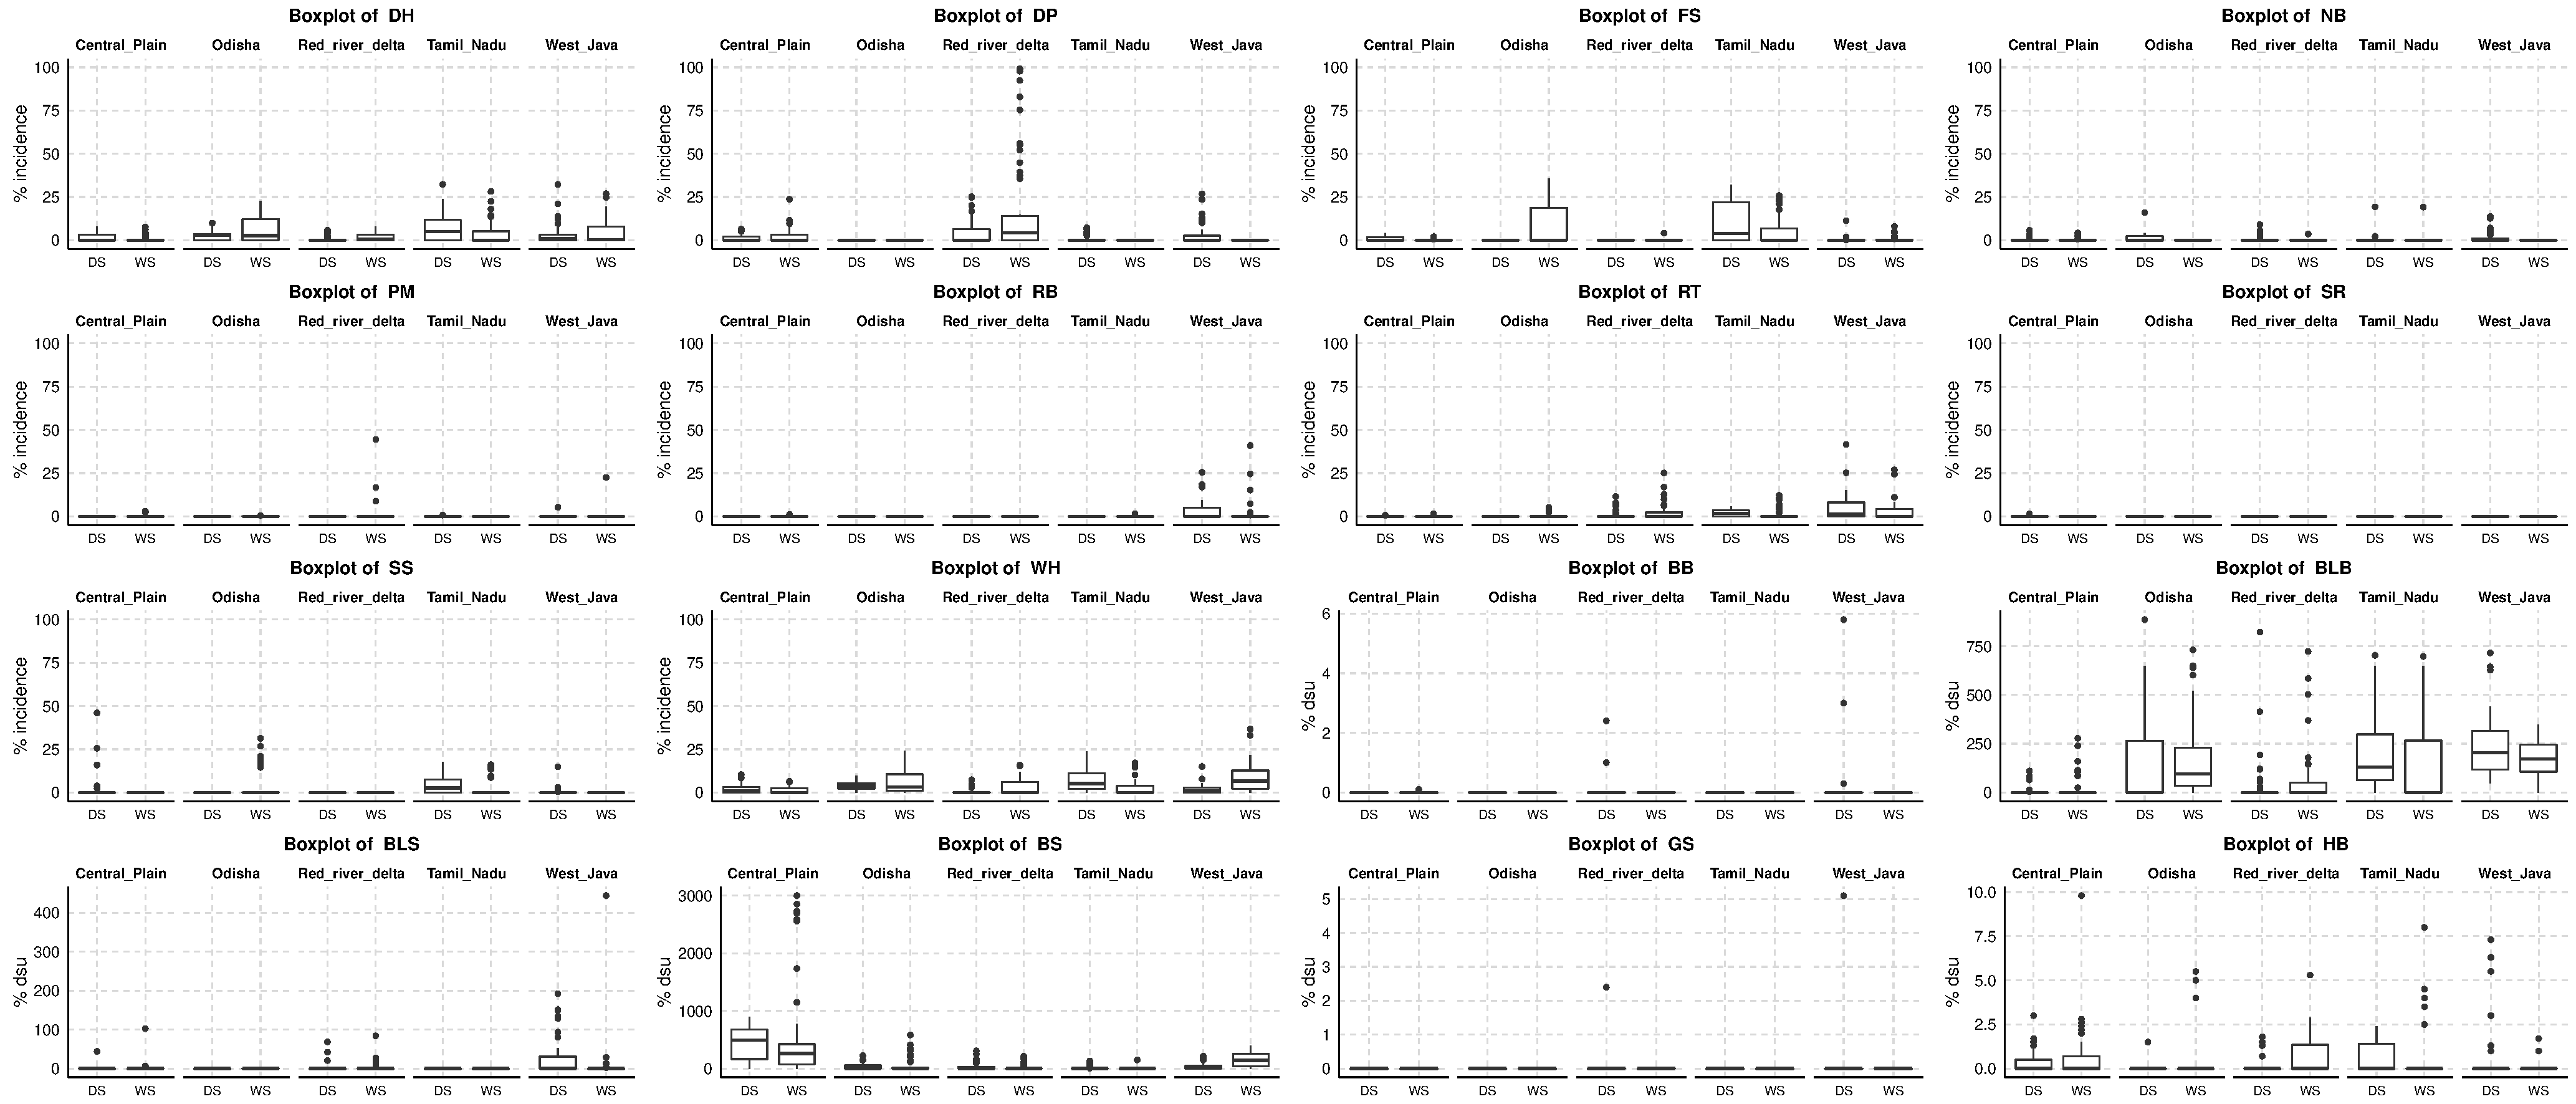
\includegraphics[height = 1\textheight]{figures/boxplot1/boxplot1.pdf}
\caption{Boxplots showing  rice injury values in crop health survey data. BB:Bug burn, BLB:Bacterial leaf blight, BLS: Bacterial leaf streak, BS:Brown spot, DH:Deadheart, DP: Dirty panicle, FS:False smut, GS:Gressy stunt, HB:Hopper burn, LB: Leaf blast, LF: Leaffolder injury, LM: Leaf miner injury, LS: :Leaf scald, NB:Neck blast, NBS:Nerrow brown spot, PM: Panicle mite injury, RB: Rice bug injuries, RGS:Ragged stunt, RH:Rice hispa injury, RS: Red stripe, RT:Rat damage, RTG: Tungro, RTH:Rice thrip injury, SHB:Sheath blight, SHR:Sheath rot, SNL:Snail damage, SR:Stem rot, SS:Silver shoot, WH:White head, WM:Whorl maggot injury.}
\label{fig:boxplot1}
\end{figure}
\end{landscape}

\begin{landscape}
\begin{figure}[!h]
\centering
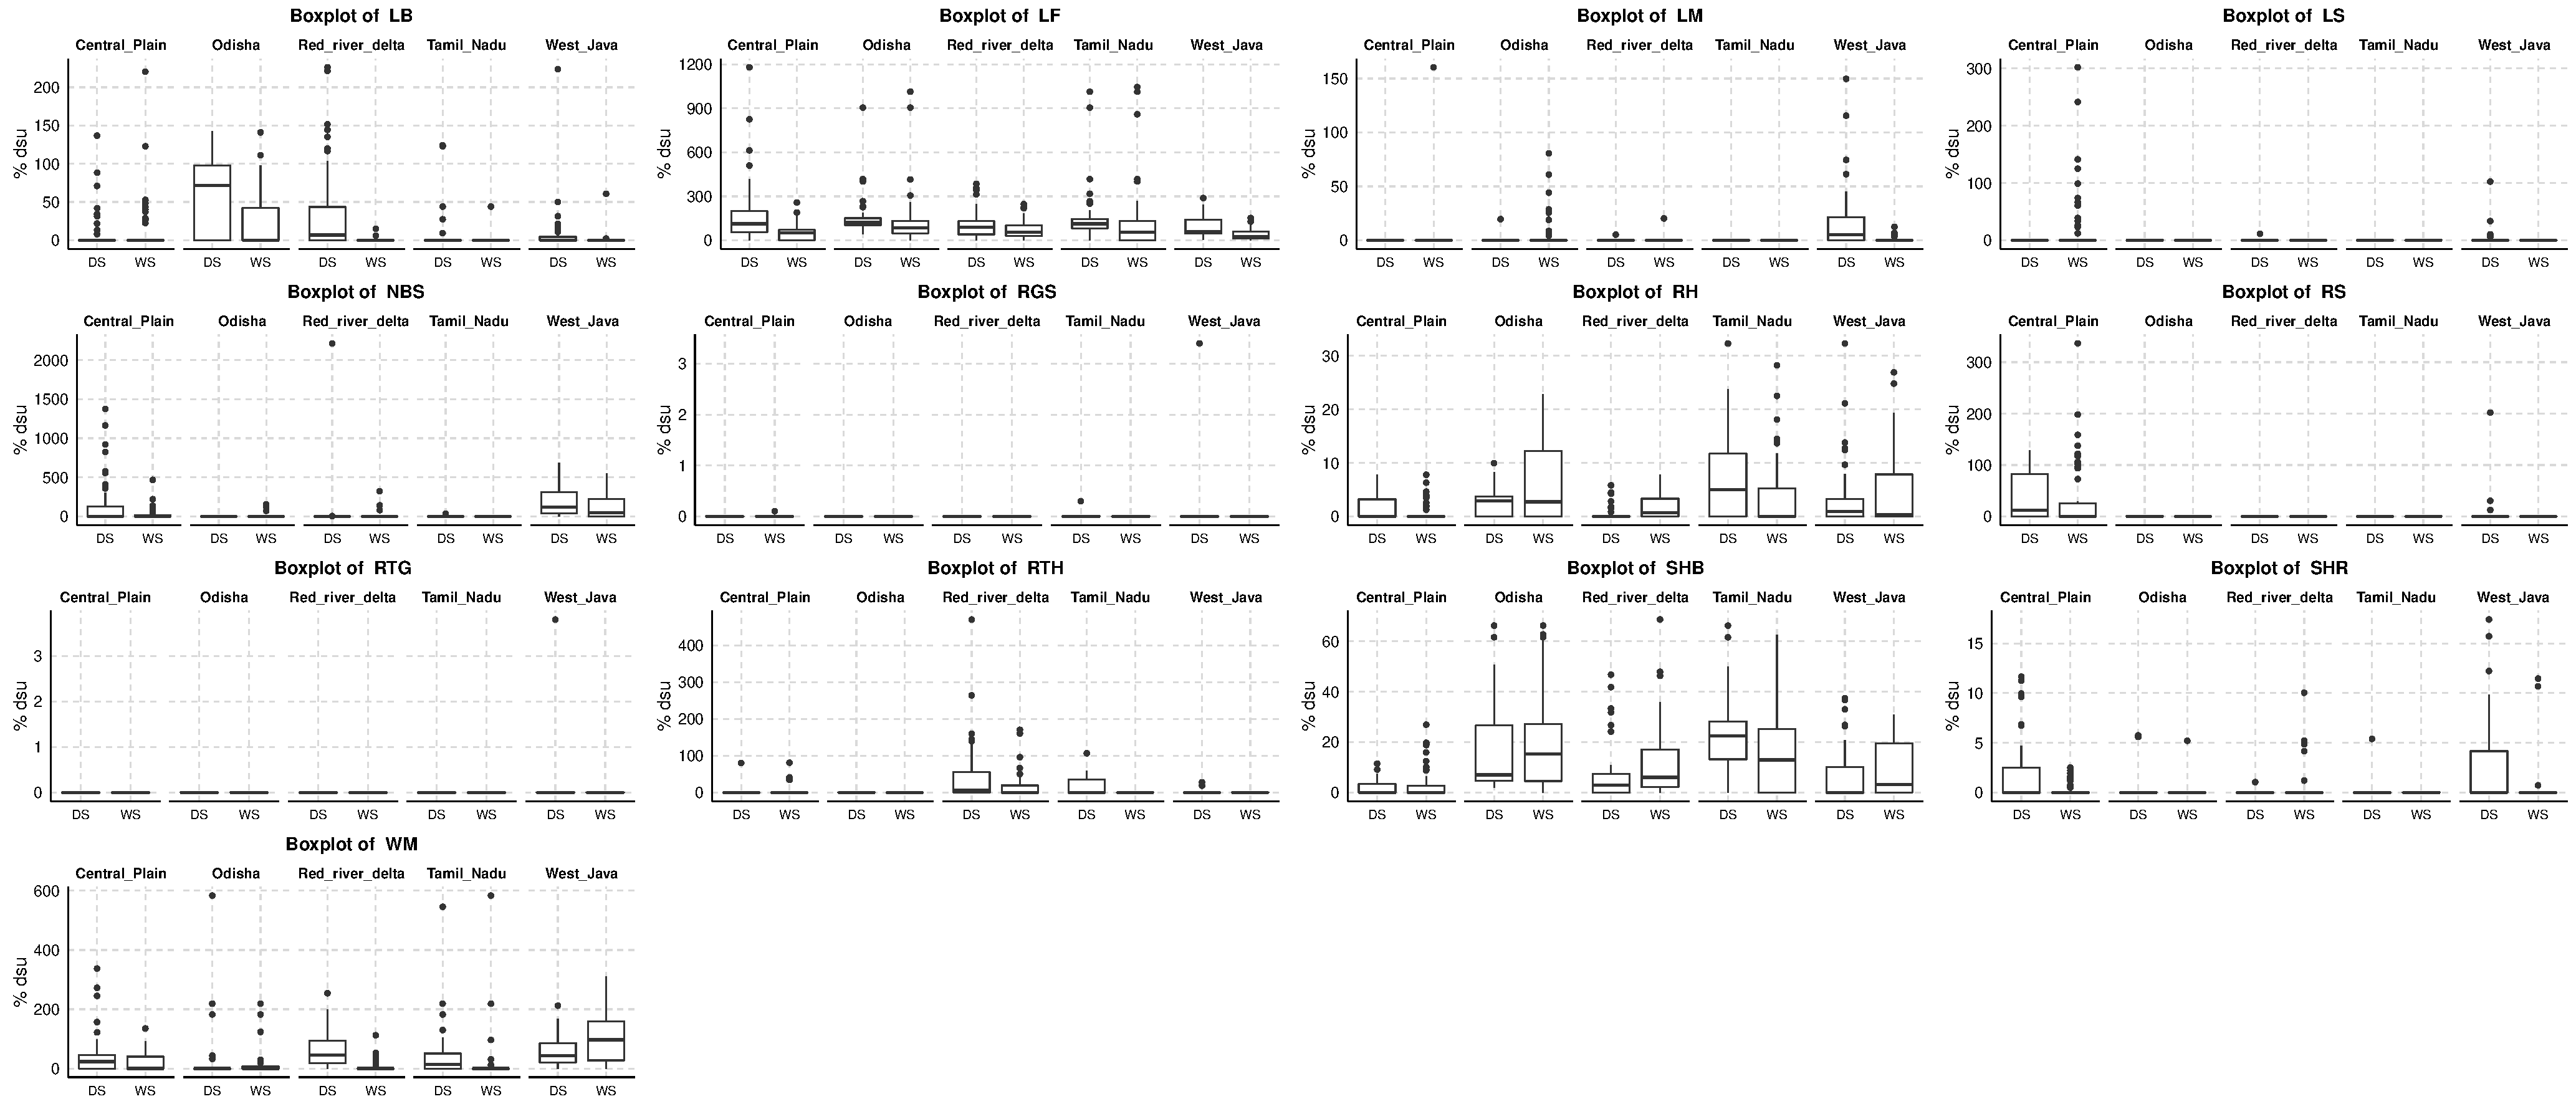
\includegraphics[height = 1\textheight]{figures/boxplot2/boxplot2.pdf}
\caption{Continue}
\label{fig:boxplot2}
\end{figure}
\end{landscape} \subsubsection{Communities, Structures and compositions of co-occurrence network of rice pest injuries}
The co-occurrence networks for theses crop health data are given in Figure to . To analyze the rice injury network, I focus on the most prominent properties of nodes in a network node: node strength, betweenness, and clustering coefficient (Figure ). Node strength is a measure of the number of connections a node has, weighted by Spearman’s correlation coefficient. Betweenness measures how often a node lies on the shortest path between every combination of two other nodes, indicating how important the node is in the flow of information through the network \citep{Opsahl_2010_Node}. The local clustering coefficient is a measure of the degree to which nodes tend to cluster together. It is defined as how often a node forms a triangle with its direct neighbors, proportional to the number of potential triangles the relevant node can form with its direct neighbors \citet{Opsahl_2010_Node}. These measures are indicative of the potential association activity through the network. As activated injuries can activate other injuries, a more densely connected network facilitates injury occurrence. Moreover, the community structure of the networks derived from the empirical data can be inspected to identify clusters of injuries or syndrome that are especially highly associated.

\begin{table}
\centering
\label{table:network_prop}
\begin{tabular}{llllll}
\hline
Production environment   & Season & Node & Edges & Average short path & Clustering coefficient \\
\hline
Central Plain, Thailand  & Dry    & 18   & 60    & 1.96               & 0.75                   \\
Central Plain, Thailand  & Wet    & 20   & 48    & 2.79               & 0.65                   \\
Odisha, India            & Dry    & 9    & 13    & 1.19               & 0.89                   \\
Odisha, India            & Wet    & 15   & 26    & 2.14               & 0.66                   \\
Red River Delta, Vietnam & Dry    & 19   & 26    & 2.15               & 0.58                   \\
Red River Delta, Vietnam & Wet    & 18   & 37    & 2.00               & 0.52                   \\
Tamil Nadu, India        & Dry    & 16   & 31    & 2.02               & 0.73                   \\
Tamil Nadu, India        & Wet    & 12   & 30    & 1.67               & 0.67                   \\
West Java, Indonesia     & Dry    & 26   & 99    & 2.14               & 0.56                   \\
West Java, Indonesia     & Wet    & 14   & 18    & 1.39               & 0.69                   \\
\hline
\end{tabular}
\end{table}
\paragraph{Central Plain, Thailand}

Dry season network (Figure \ref{fig:networkCP_ds}) was composed of 18 associated injuries and captured 60 associations (edges). The network showed two groups of injury syndromes (the combination of injuries) based on the optimal clustering algorithm. The group1 (green) was more closely clustered than another group, according to node properties, the injuries in group1 had high clustering coefficient such as WH, SHR, SHB, DP, BS, RH, NB, DH, FS, HB, and RS. This indicated that these injuries formed complex co-occurrence relationships. Network properties (Figure \ref{fig:nodepropCP_ds}) showed that WM and LF, BS, BLB, NBS are high-betweenness nodes.  As opposed to other injuries, LB and BLS had low scores on two from three centrality measure. Apparently, LB less possibly co-occur with other injuries (low betweenness), and did not co-occur with other injuries (low degree and clustering coefficient).

In wet season, the co-occurrence network of rice injuries (Figure \ref{fig:networkCP_ws}) reveals 4 syndromes, 20 injuries, and 48  significant relationships (edges). Group3 (purple) is composed of BLS, RS, HB, SHB, SHR and WM. They were closer to each other than other groups based on the structure and clustering coefficient (Figure \ref{fig:nodepropCP_ws}). The members of this group such as WM, HB, SHB, RS also had high node degree, which indicated that when they occurred, injuries in symdrome2 (orange) tend to occur because of their associations. Group4 (pink) connected only to syndrome3, so the injuries in syndrome4 depended on the injuries of syndrome3, and were less likely to occur in this season.  RT and RB were less likely to occur in this season because of low centrality, if they presented in rice fields, other injuries had low tendency to occur. 

\begin{figure}
    \centering
    \begin{subfigure}[b]{1\textwidth}
        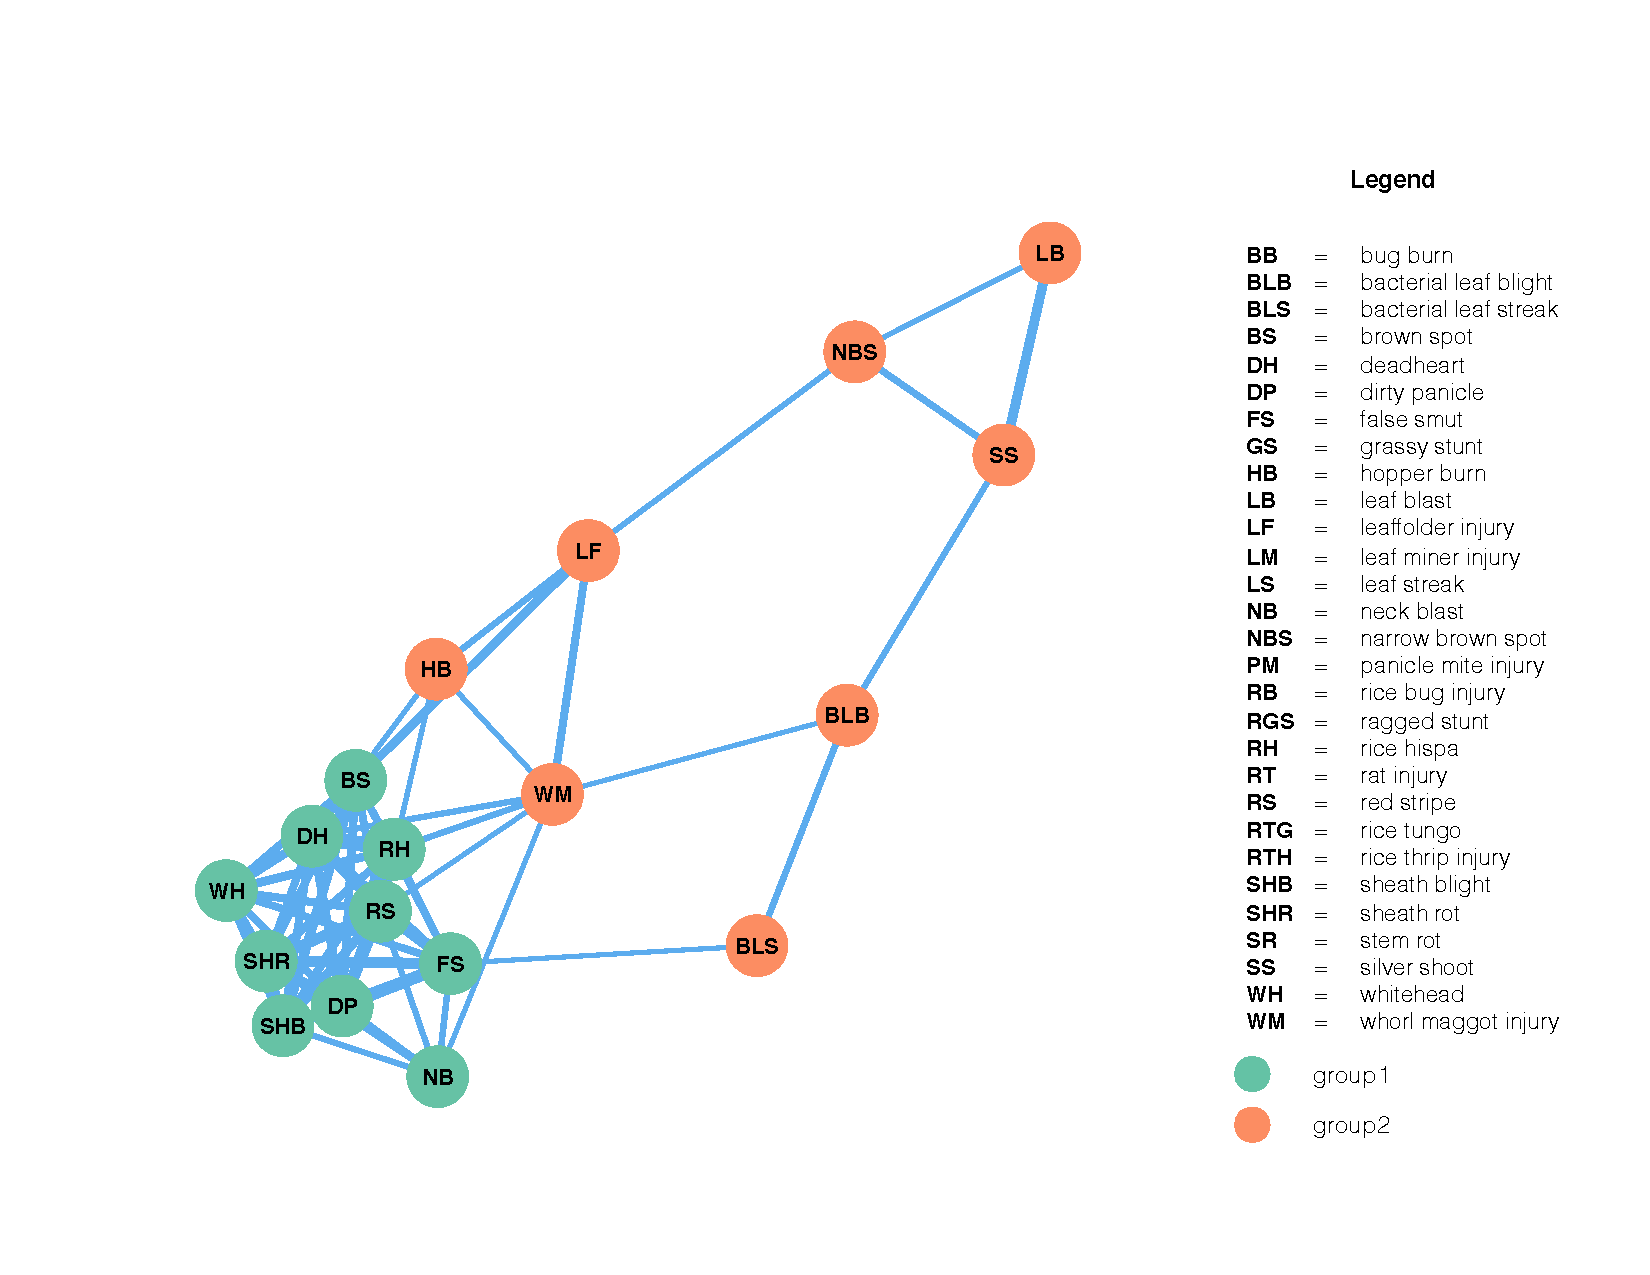
\includegraphics[width = 1\textwidth]{figures/networkCP_ds/networkCP_ds.pdf}
        \caption{Co-occurrence network of rice injuries in dry season at Central Plain, Thailand. The layout of the network graph is based on the Fruchterman-Reingold algorithm, which places nodes with stronger or more connections closer to each other.}
        \label{fig:networkCP_ds}
    \end{subfigure}
    \begin{subfigure}[b]{1\textwidth}
        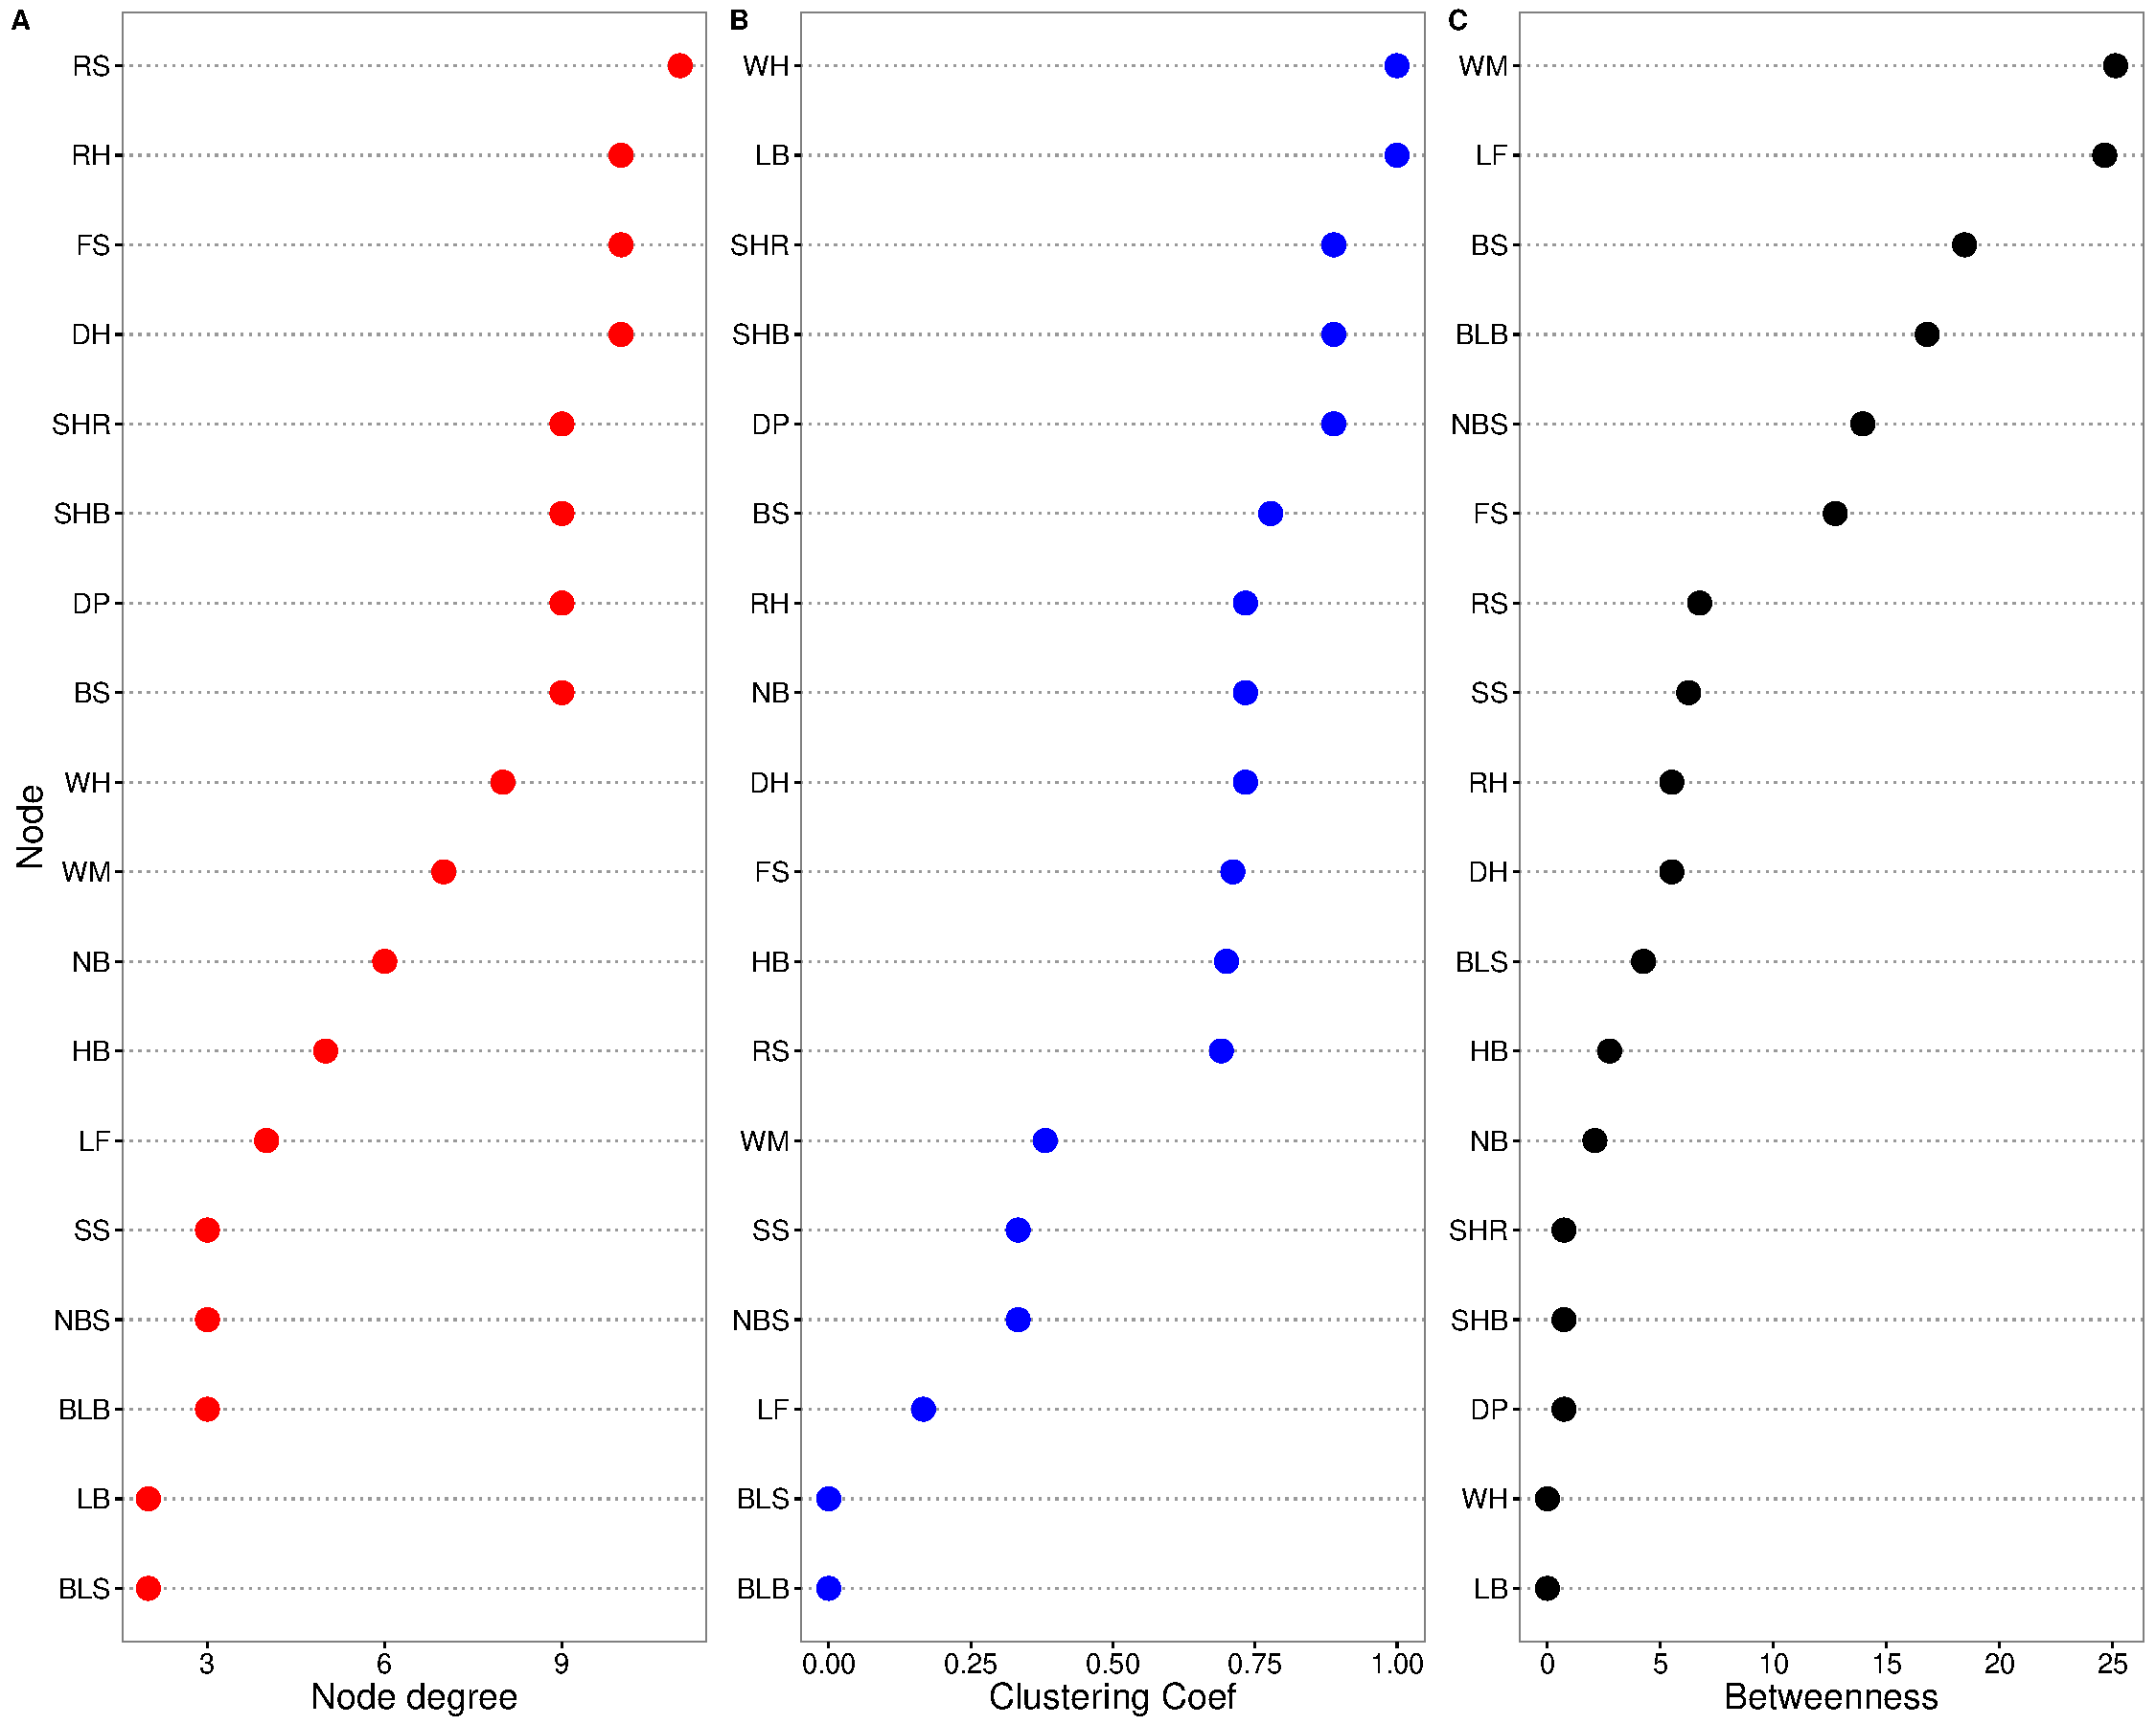
\includegraphics[width = 1\textwidth]{figures/nodepropCP_ds/nodepropCP_ds.pdf}
        \caption{Three centrality measures of the nodes in co-occurrence network of rice injuries in dry season at Central Plain. A: node degree, B:clustering coefficient, and C:Betweenness.}
        \label{fig:nodepropCP_ds}
    \end{subfigure}
    \caption{Rice injuries in dry season in Central Plain, Thailand}
    \label{fig:CP_ds}
\end{figure}

\begin{figure}
    \centering
    \begin{subfigure}[b]{1\textwidth}
        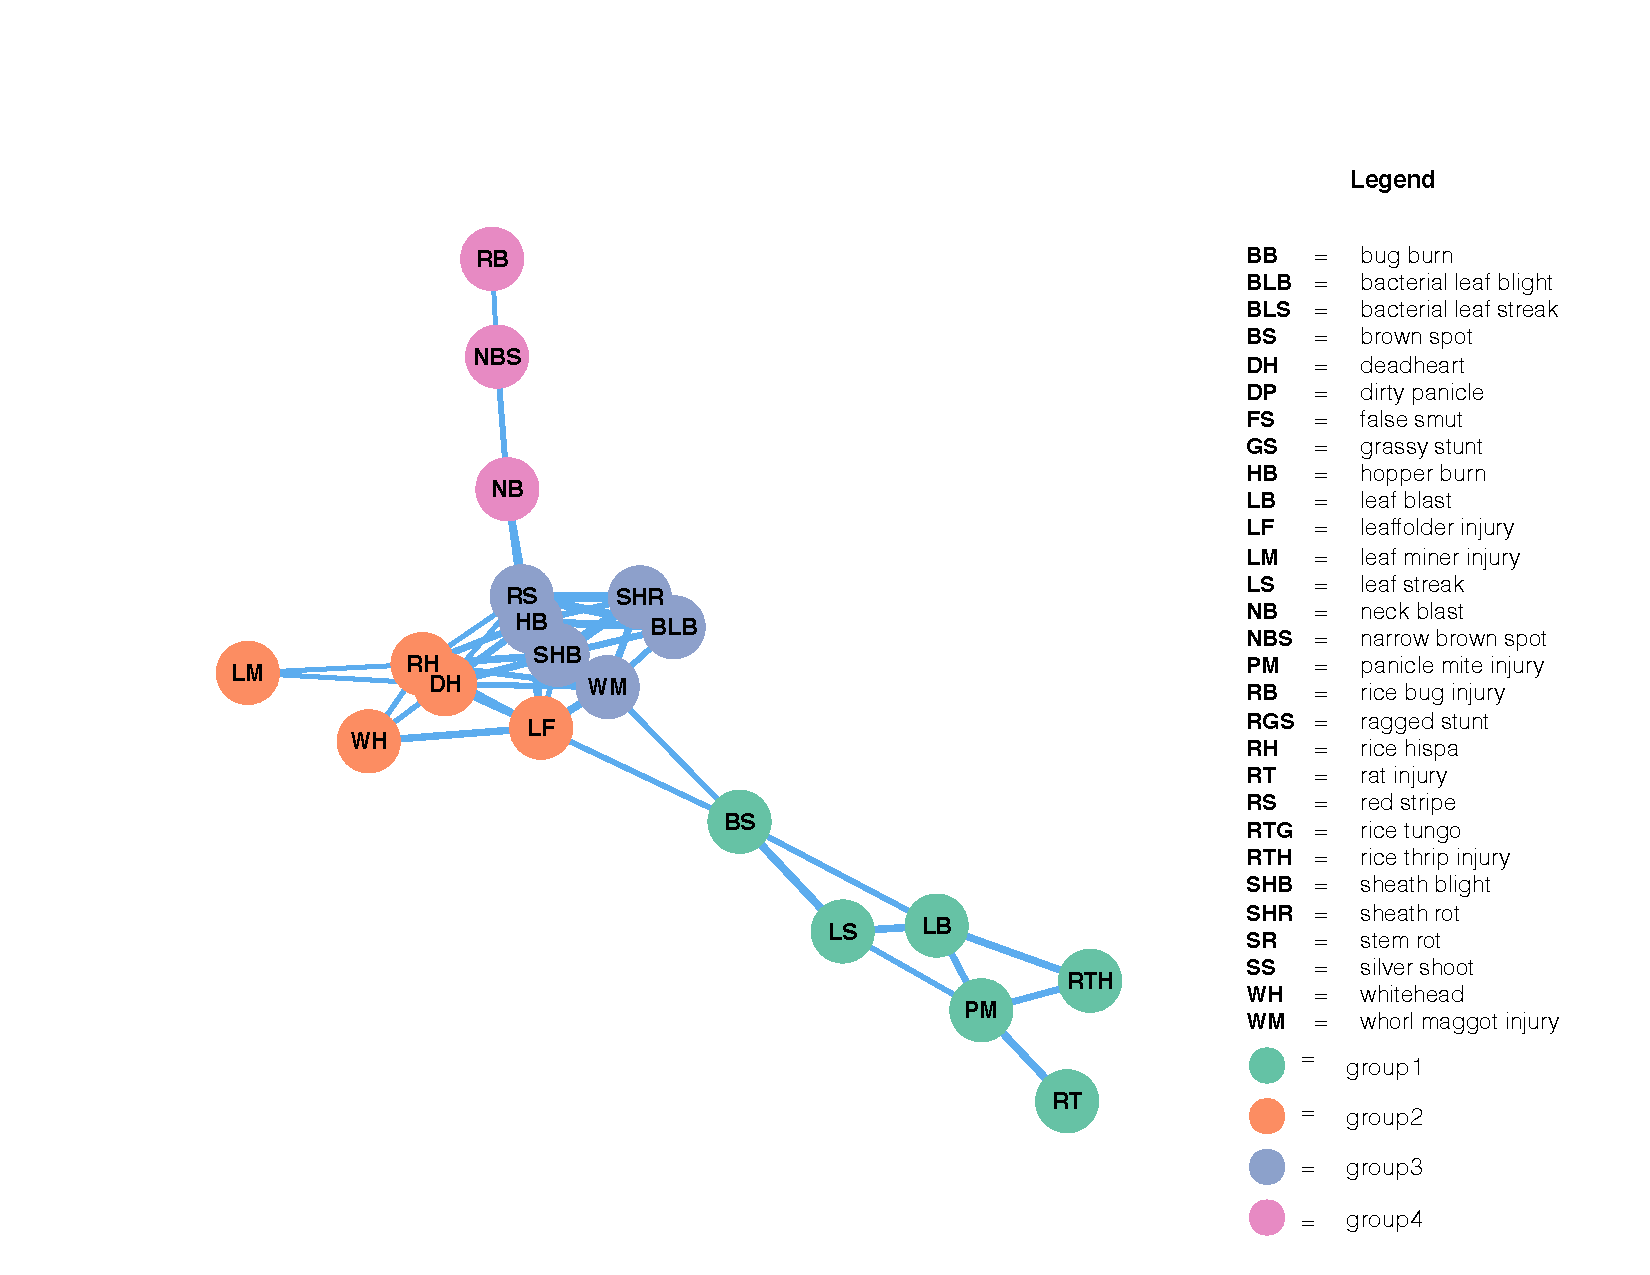
\includegraphics[width = 1\textwidth]{figures/networkCP_ws/networkCP_ws.pdf}
        \caption{Co-occurrence network of rice injuries in dry season at Central Plain, Thailand. The layout of the network graph is based on the Fruchterman-Reingold algorithm, which places nodes with stronger or more connections closer to each other.}
        \label{fig:networkCP_ws}
    \end{subfigure}
    \begin{subfigure}[b]{1\textwidth}
        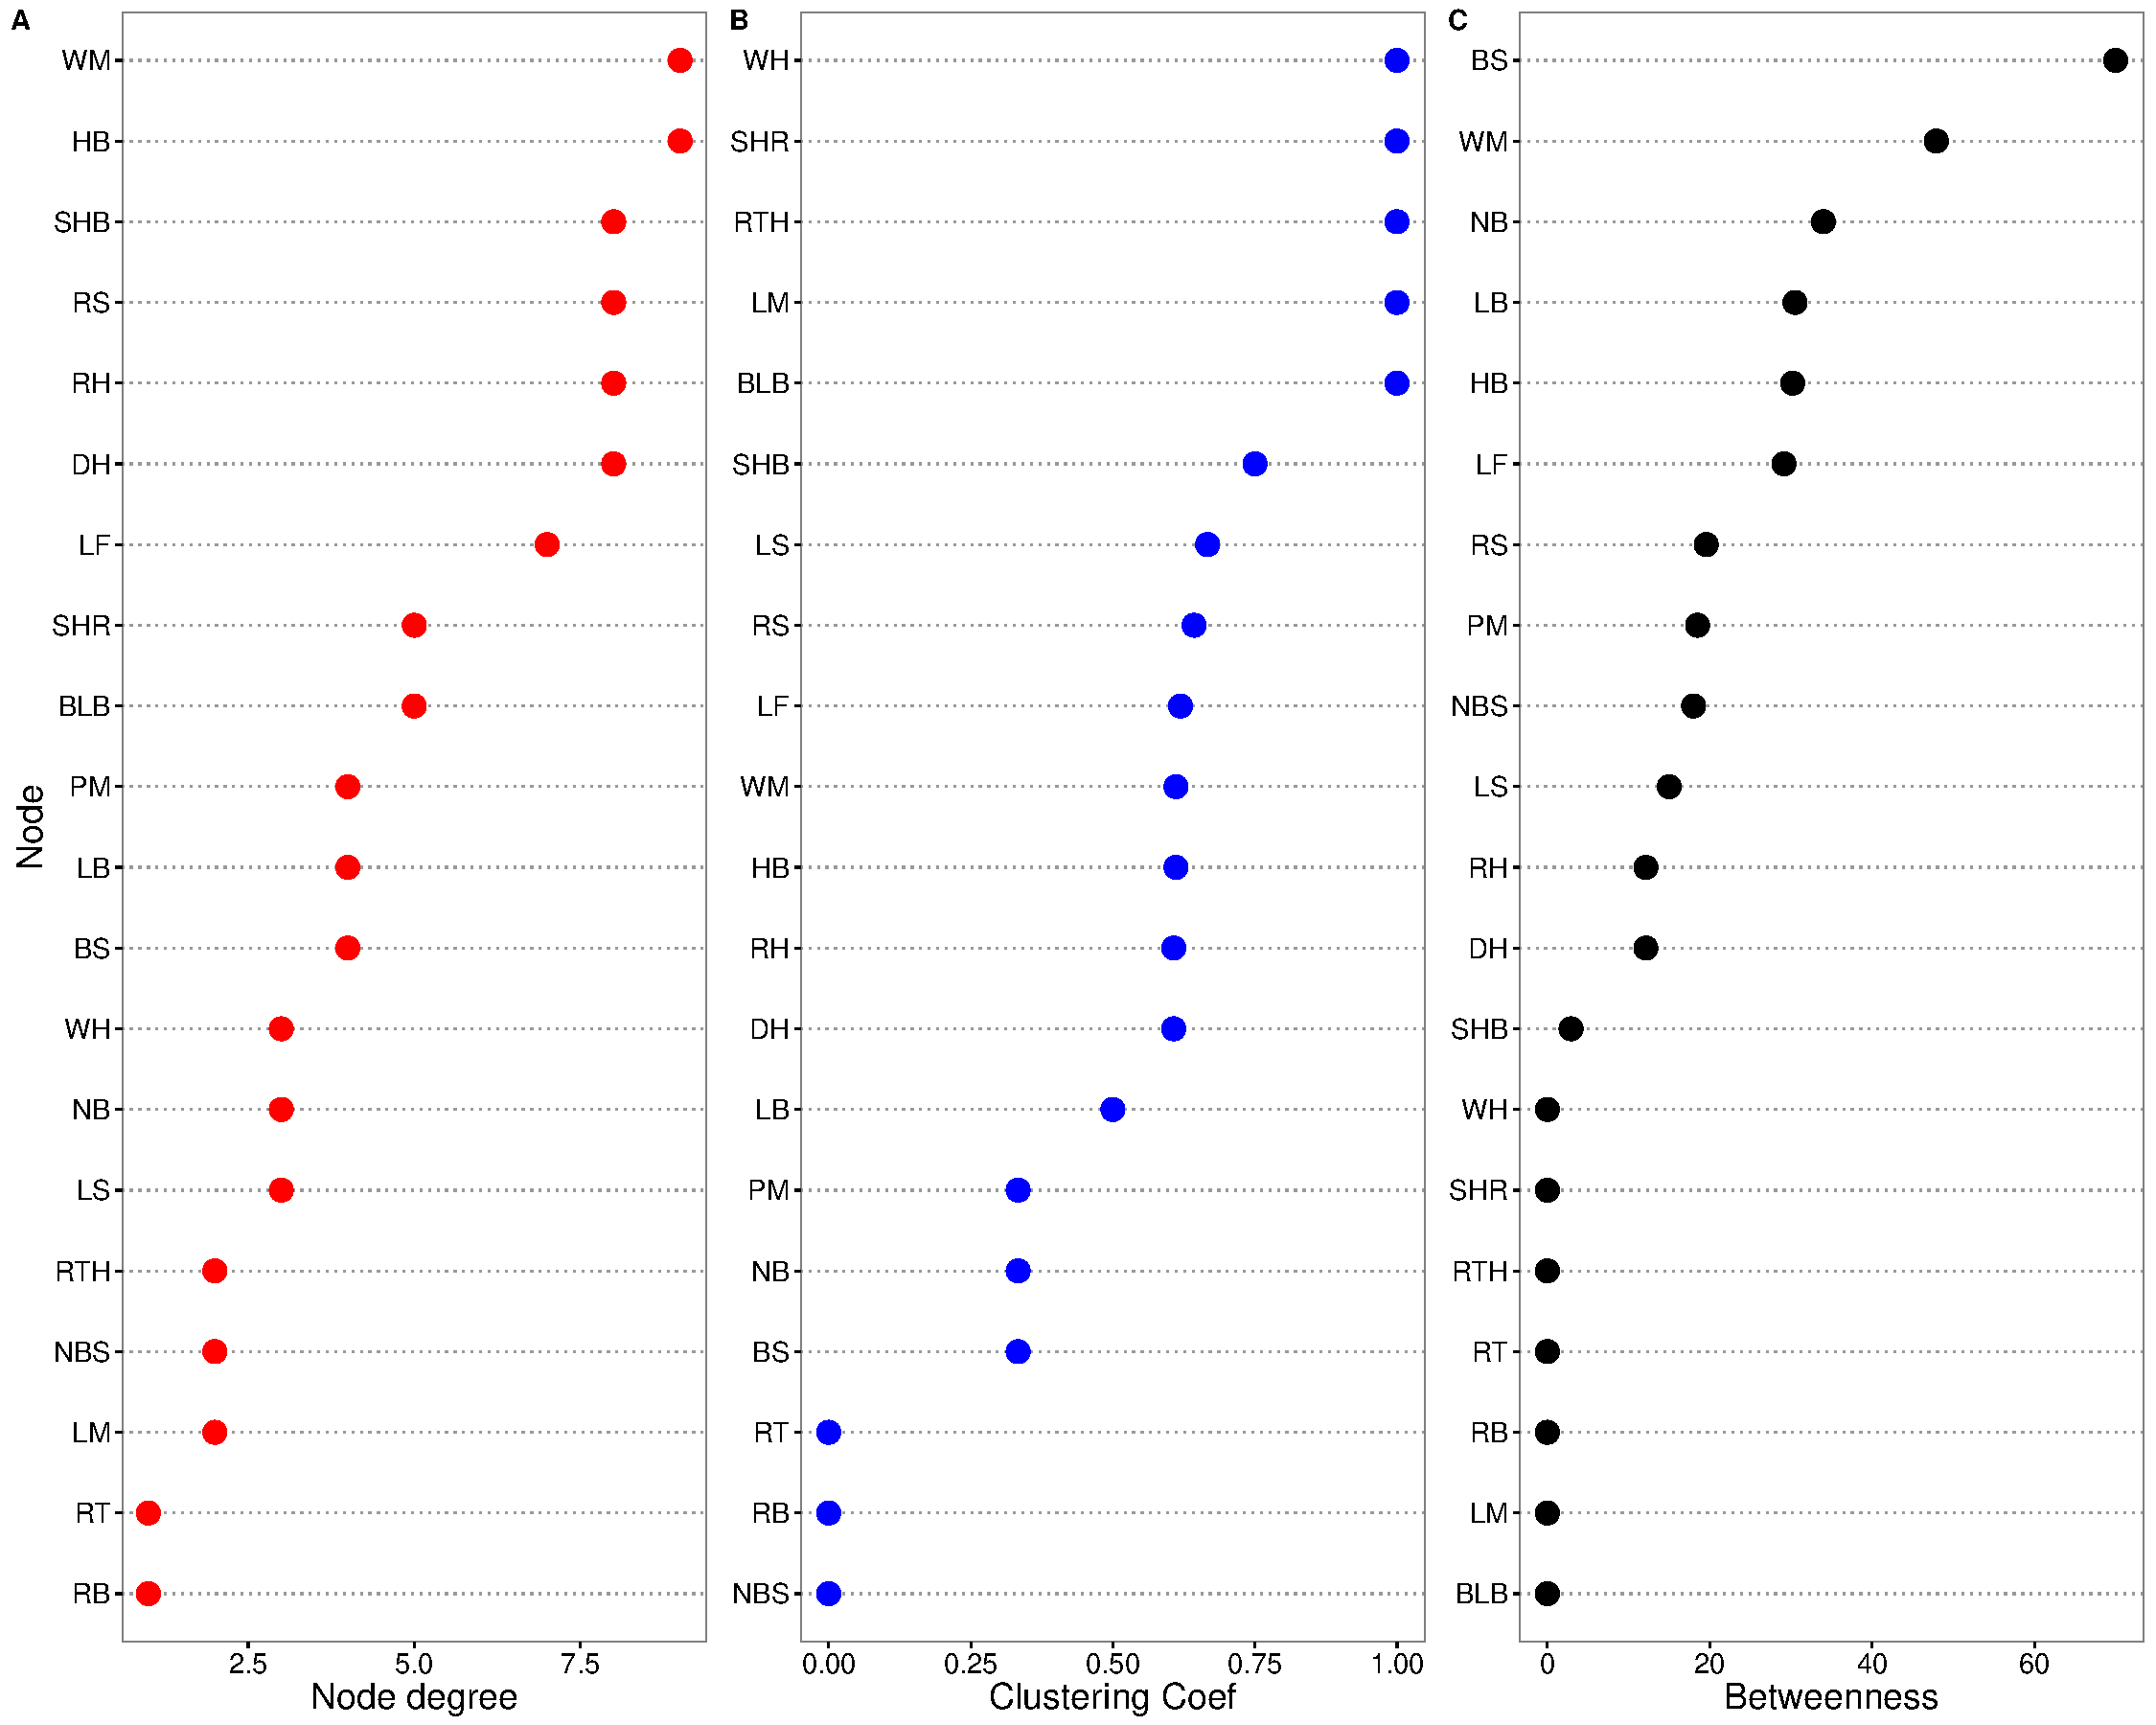
\includegraphics[width = 1\textwidth]{figures/nodepropCP_ws/nodepropCP_ws.pdf}
        \caption{Three centrality measures of the nodes in co-occurrence network of rice injuries in dry season at Central Plain. A: node degree, B:clustering coefficient, and C:Betweenness}
        \label{fig:nodepropCP_ws}
    \end{subfigure}
    \caption{Injuries in Central Plain, Thailand}
    \label{fig:CP_ws}
\end{figure}

\paragraph{Odisha, India}

Co-occurrence network of rice injuries in dry season (Figure \ref{fig:networkOR_ds}) was composed of 9 associated injuries and captured 13 associations. The network showed two isolated groups of injuries. Injuries within groups were closely related based on clustering coefficient (Figure \ref{fig:nodepropOR_ds}). This network could be inferred that there are two injury syndromes. One was the combination of BS, BLB, WM and SHB. Another was RH, WH, DH, LB, NB.

The network in wet season (Figure \ref{fig:networkOR_ws}) was more complex than dry season one. It composed of 15 nodes with 26 edges. The network reveals four groups of injury profiles. Group4 was isolated from the rest. Group2 was the biggest group placed in the middle of group1 and 3. The injuries in group2 had high node degree (Figure \ref{fig:nodepropOR_ws}), which mean they were connected to many injuries. NBS and LF, injuries in group1 and group2, respectively presented high betweenness values and connected to injuries of group3. This indicated that group3 injuries had high chance to occur together with group1 and 2, but not group4. 

\begin{figure}
    \centering
    \begin{subfigure}[b]{1\textwidth}
        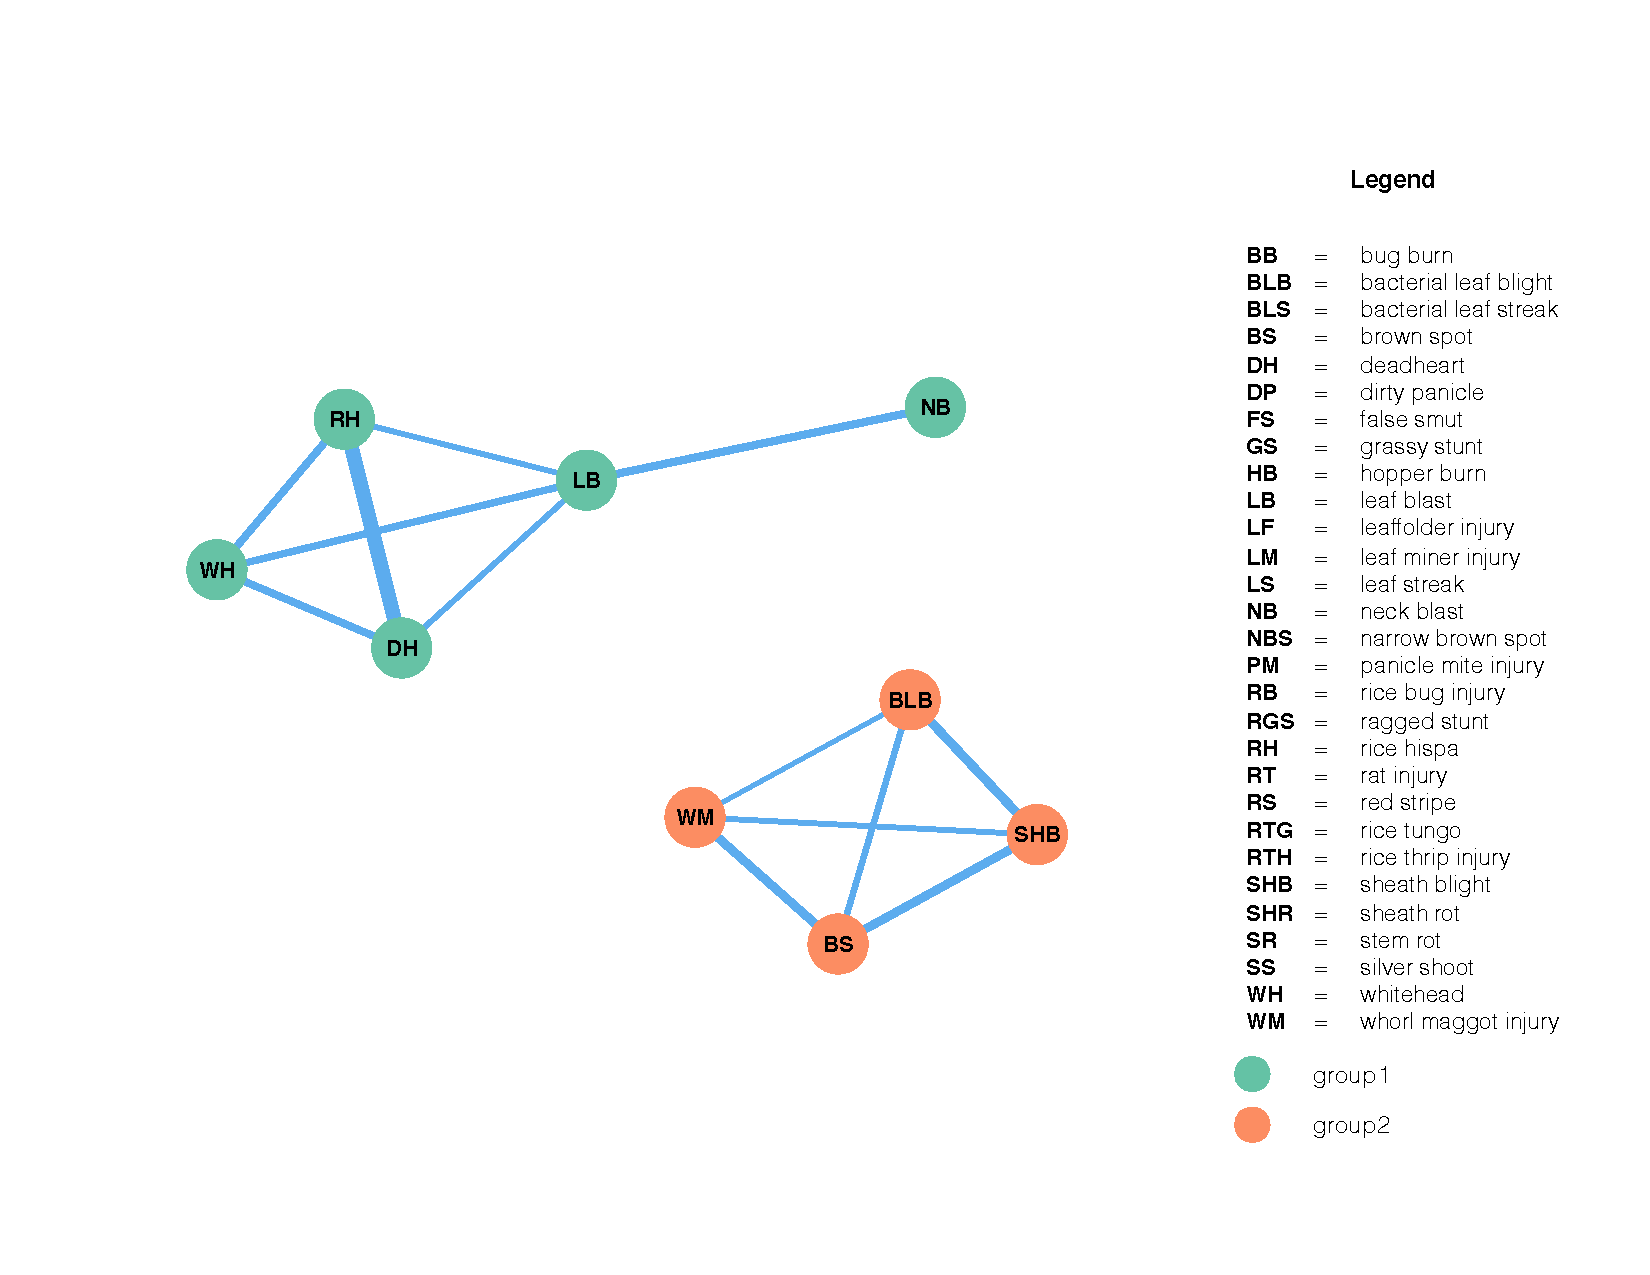
\includegraphics[width = 1\textwidth]{figures/networkOR_ds/networkOR_ds.pdf}
        \caption{Co-occurrence network of rice injuries in wet season at Odisha, India. The layout of the network graph is based on the Fruchterman-Reingold algorithm, which places nodes with stronger or more connections closer to each other.}
        \label{fig:networkOR_ds}
    \end{subfigure}
    \begin{subfigure}[b]{1\textwidth}
        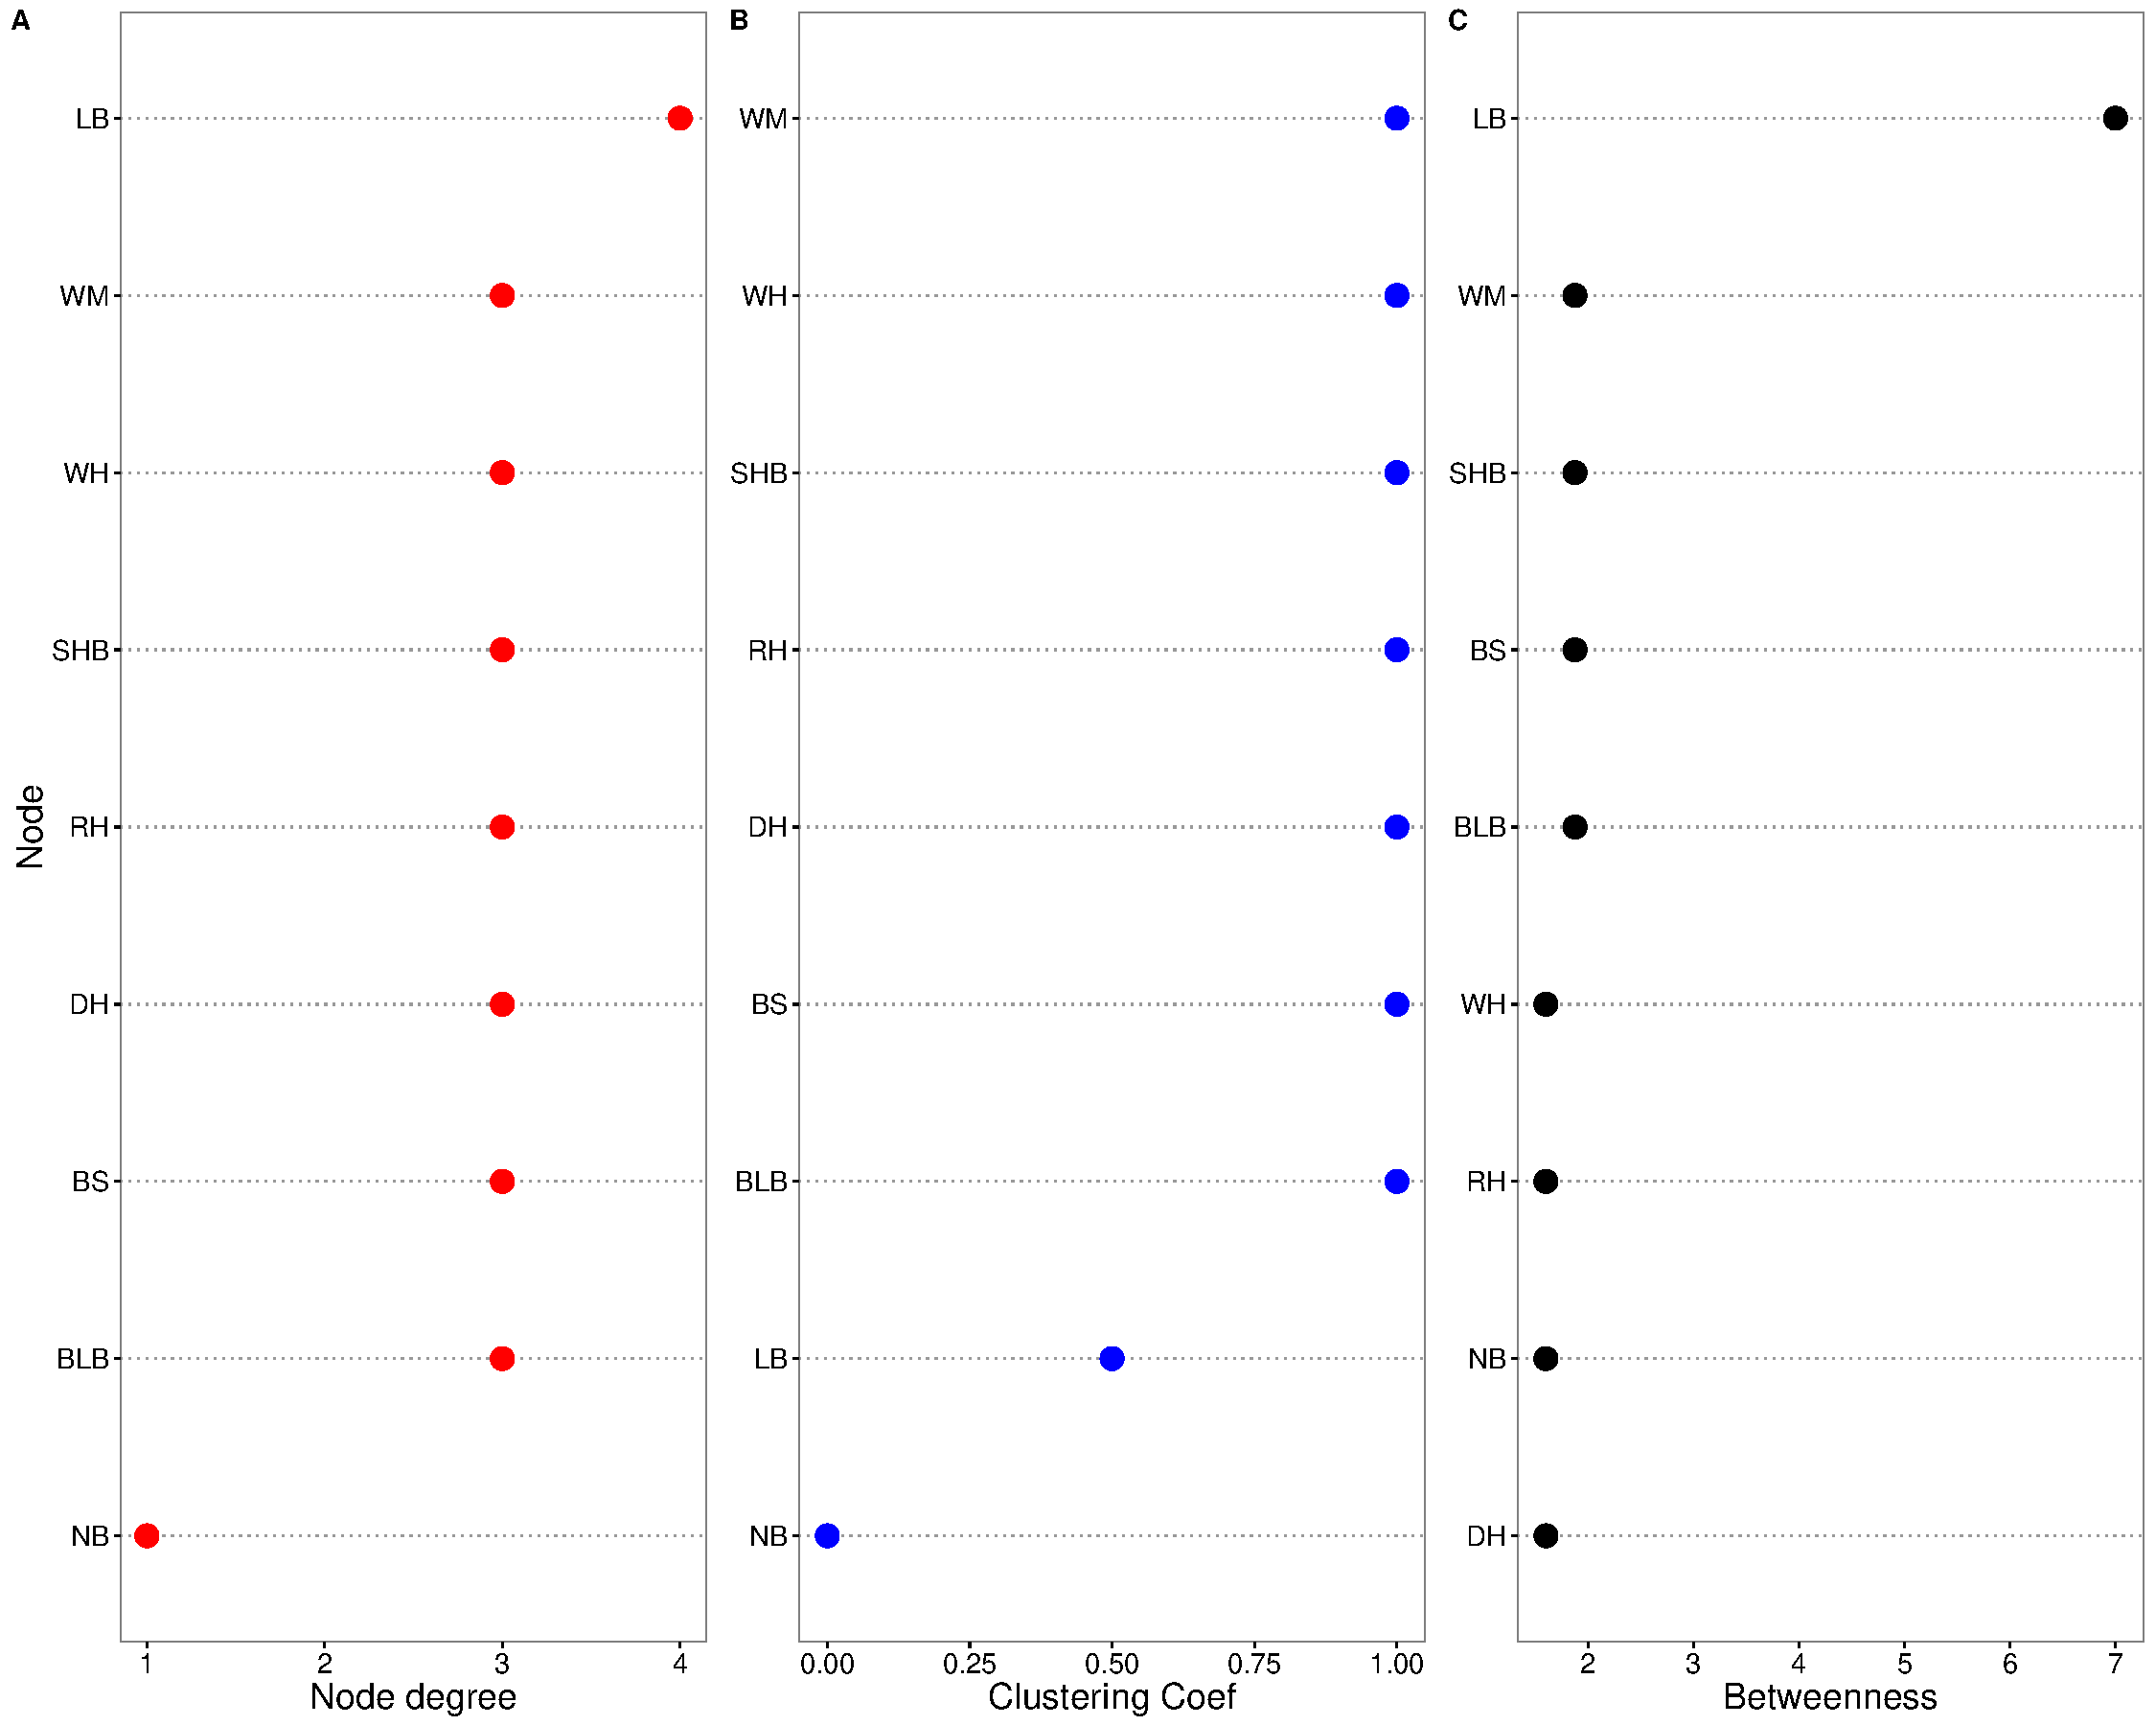
\includegraphics[width = 1\textwidth]{figures/nodepropOR_ds/nodepropOR_ds.pdf}
        \caption{Three centrality measures of the nodes in co-occurrence network of rice injuries in dry season at Odisha, India. A: node degree, B:clustering coefficient, and C:Betweenness.}
        \label{fig:nodepropOR_ds}
    \end{subfigure}
    \caption{Injuries in dry season at Odisha, India}
    \label{fig:OR_ds}
\end{figure}

\begin{figure}
    \centering
    \begin{subfigure}[b]{1\textwidth}
        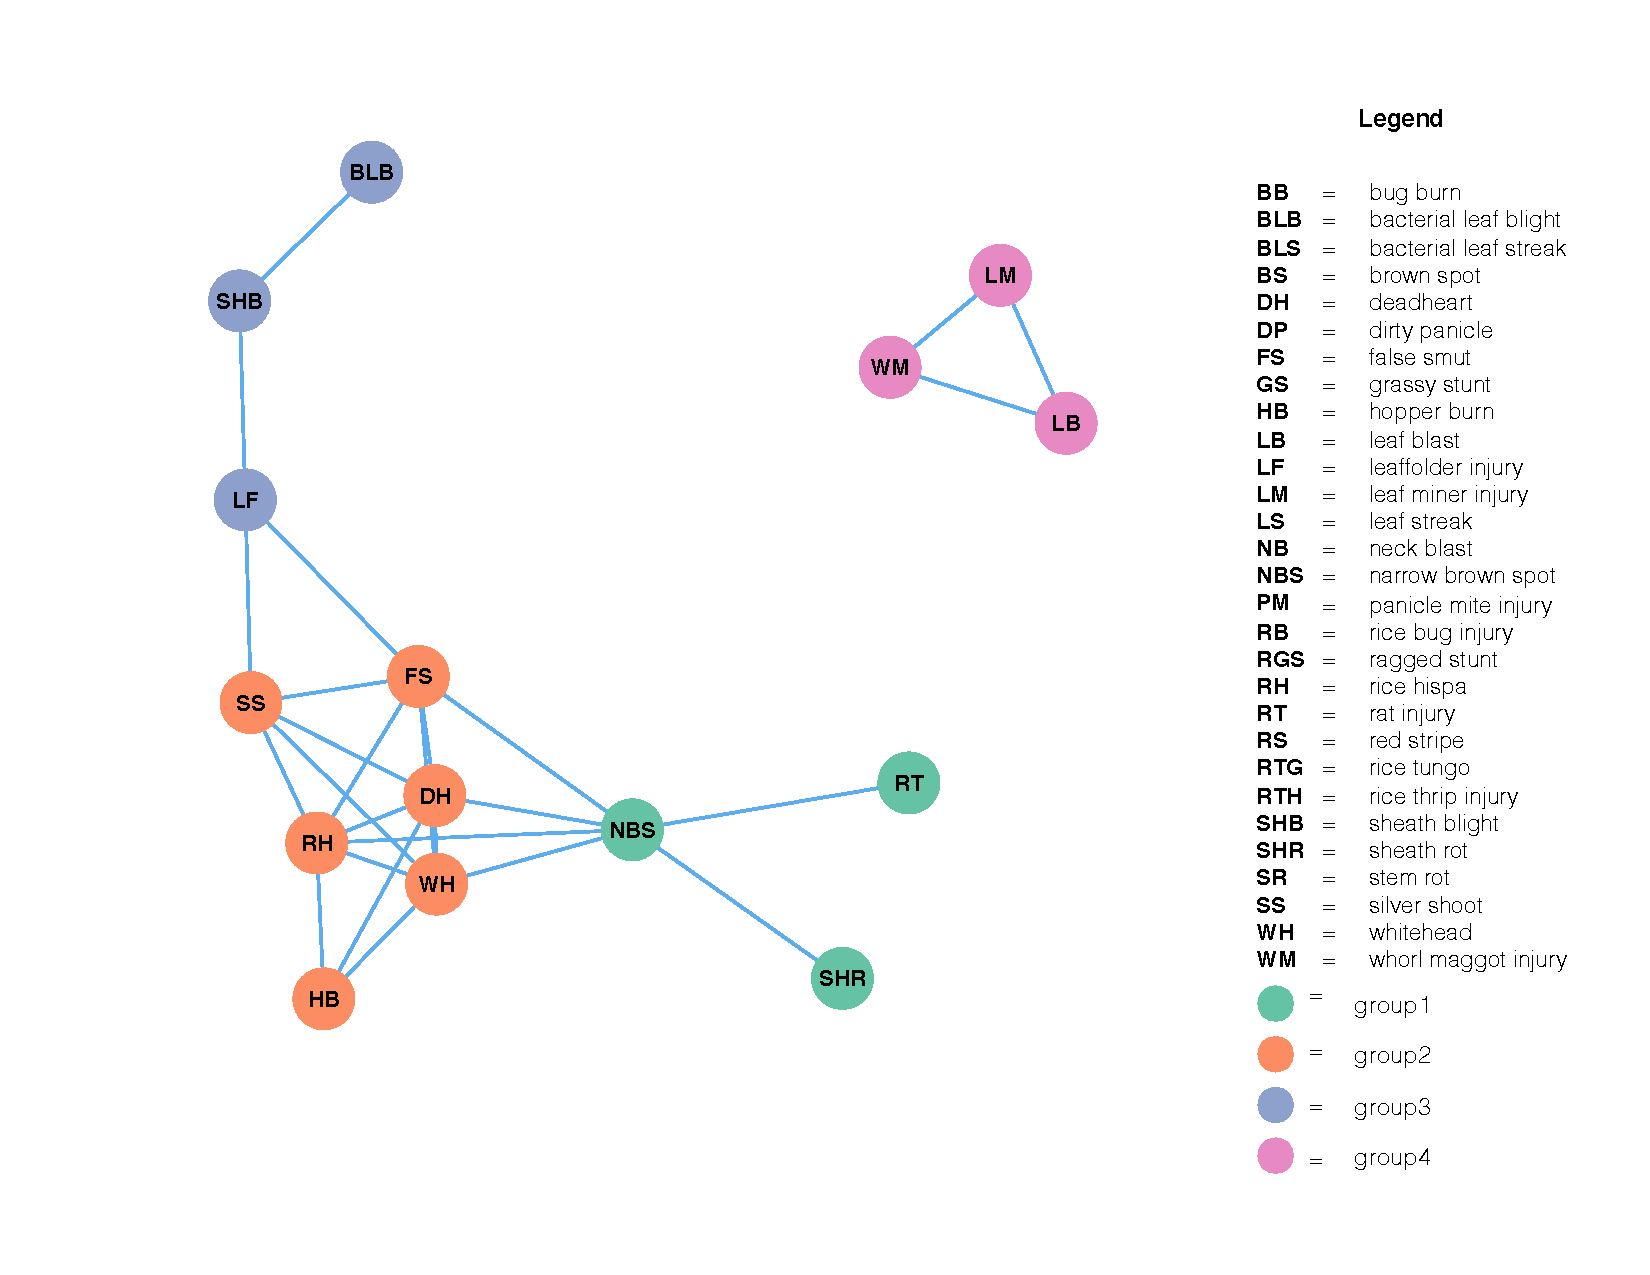
\includegraphics[width = 1\textwidth]{figures/networkOR_ws/networkOR_ws.pdf}
        \caption{Co-occurrence network of rice injuries in wet season at Odisha, India. The layout of the network graph is based on the Fruchterman-Reingold algorithm, which places nodes with stronger or more connections closer to each other.}
        \label{fig:networkOR_ws}
    \end{subfigure}
    \begin{subfigure}[b]{1\textwidth}
        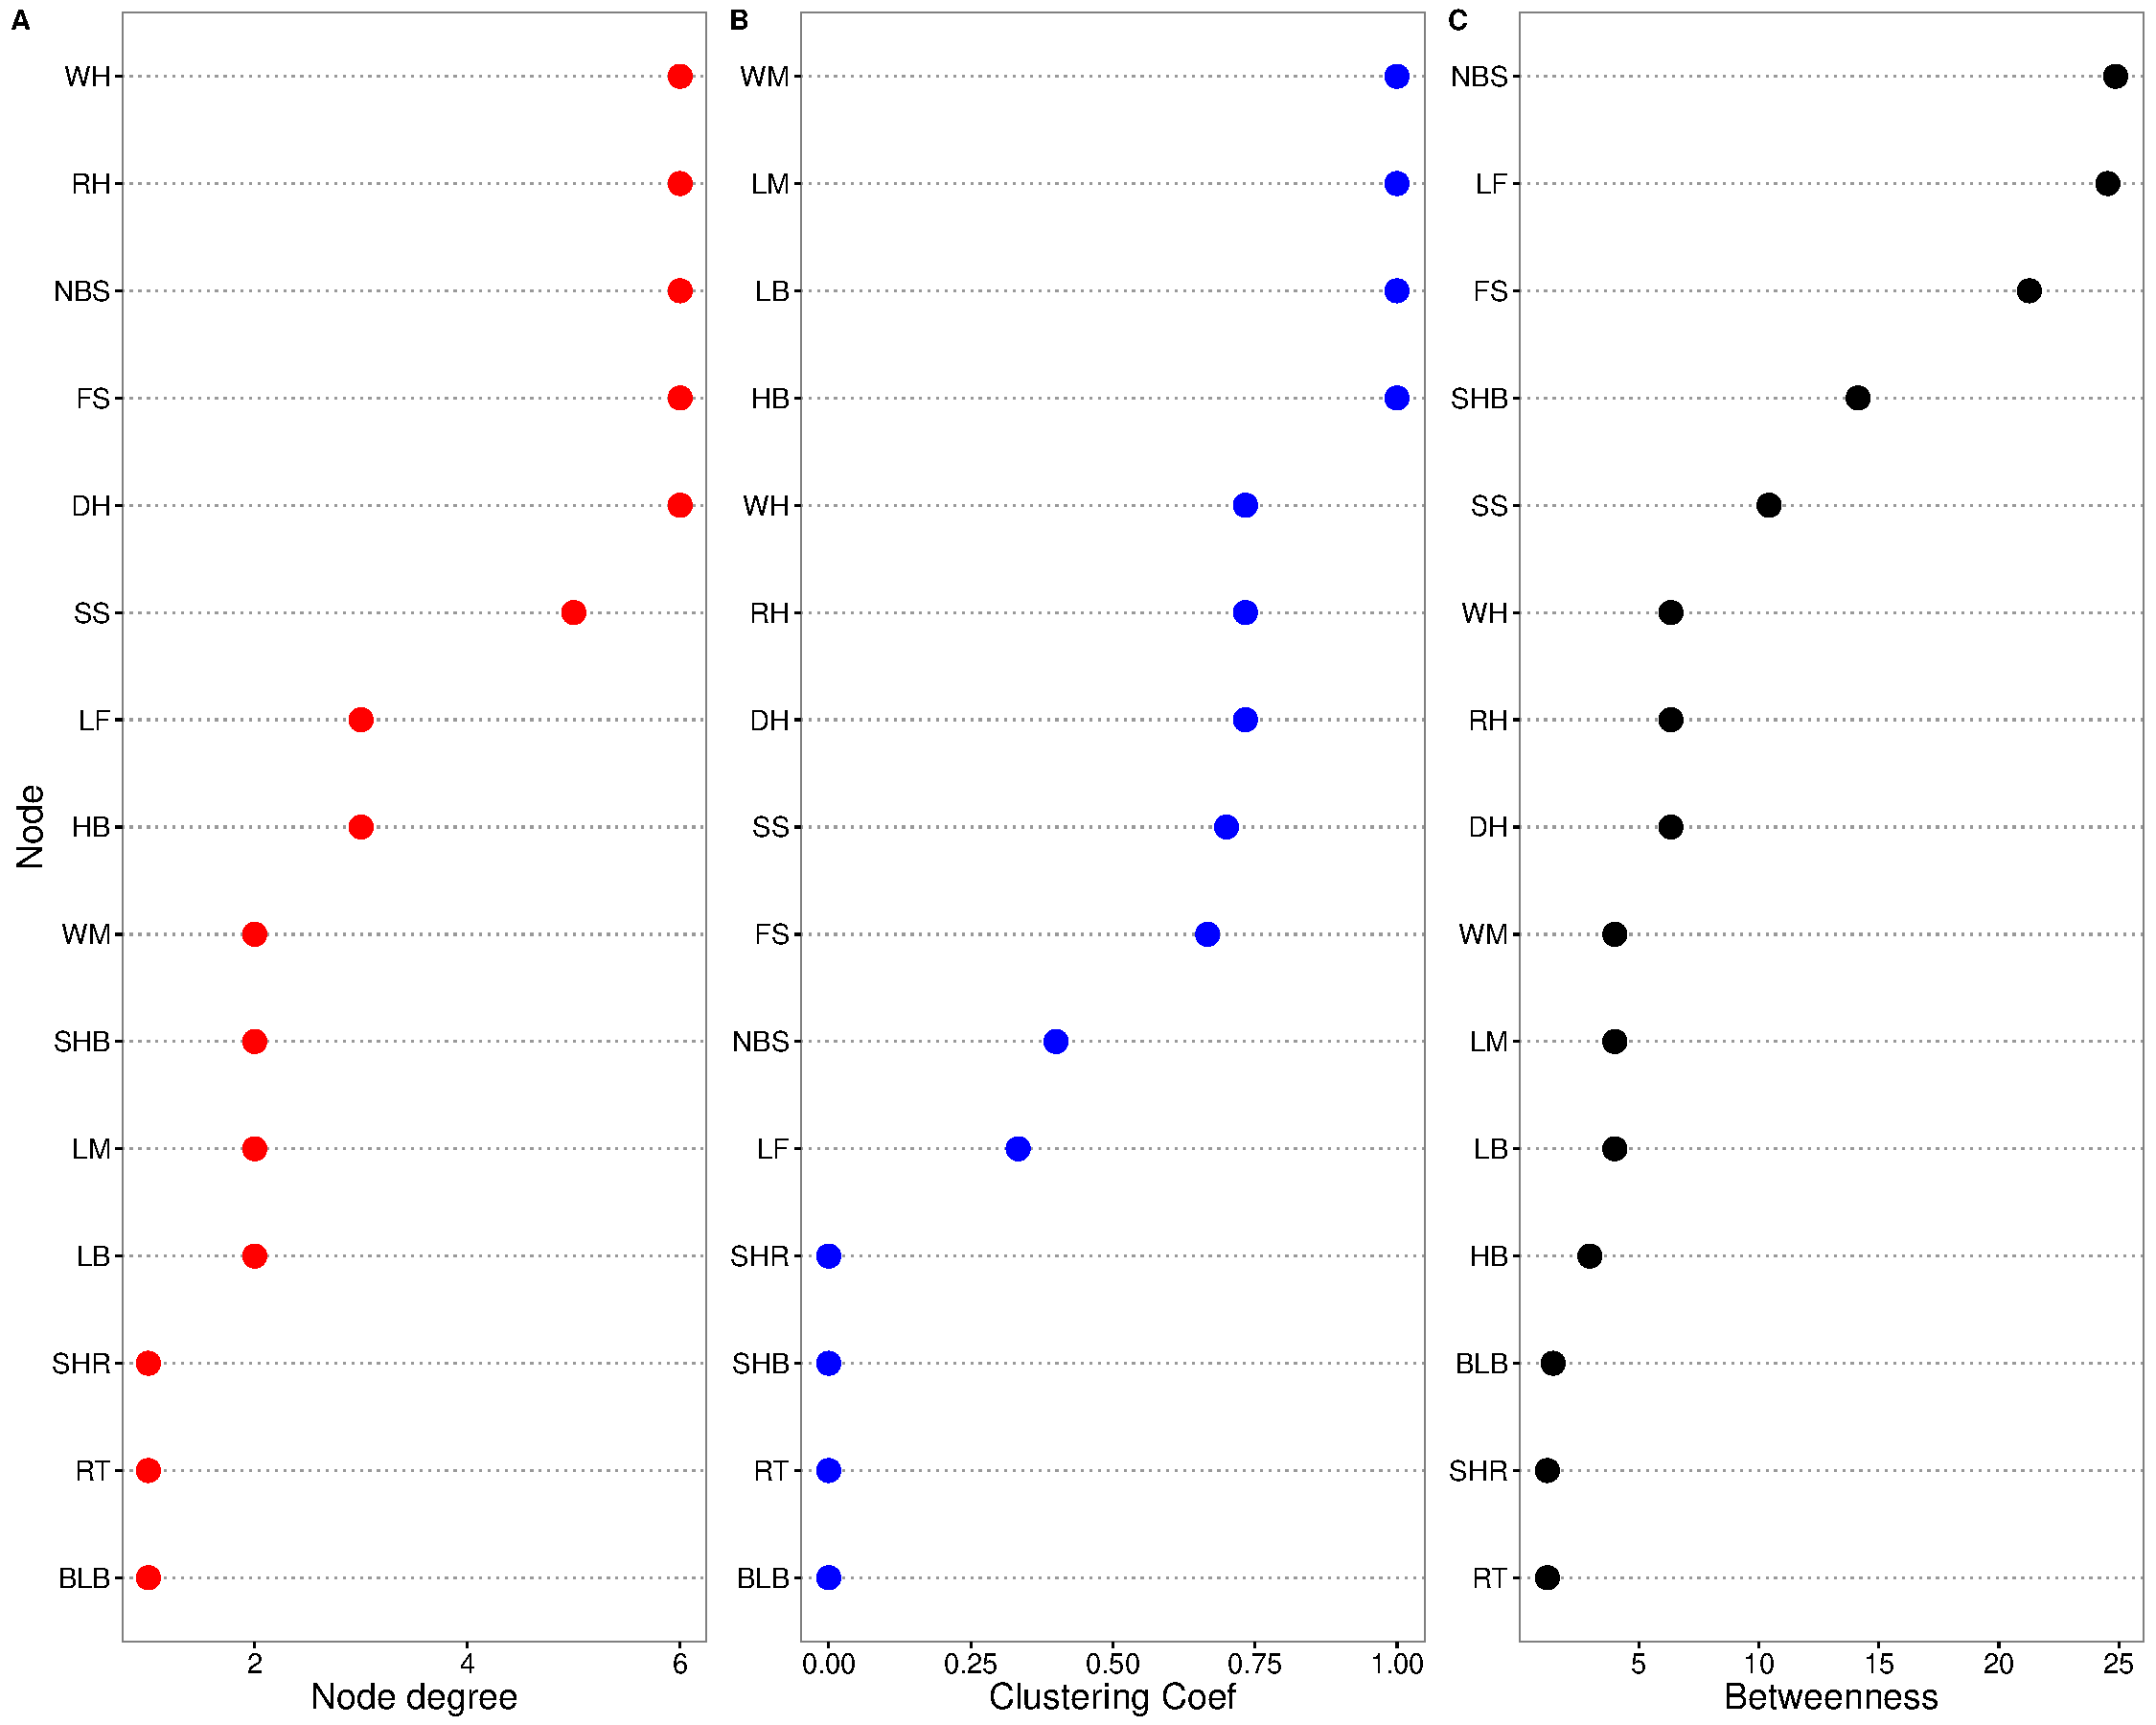
\includegraphics[width = 1\textwidth]{figures/nodepropOR_ws/nodepropOR_ws.pdf}
        \caption{Three centrality measures of the nodes in co-occurrence network of rice injuries in wet season at Odisha, India. A: node degree, B:clustering coefficient, and C:Betweenness.}
        \label{fig:nodepropOR_ws}
    \end{subfigure}
    \caption{Injuries in wet season at Odisha, India}
    \label{fig:OD_ws}
\end{figure}


\paragraph{Red River Delta, Vietnam}
 
Co-occurrence network of rice injuries in dry season (Fig. \ref{fig:networkRR_ds}) composed of 19 nodes and 26 associations. The network reveals three isolated groups, and two connected groups of injury profiles. Group1 and group3 were linked with BB. Group3 was the biggest among the others. In this group, SHB, BS were nodes showing high centrality (Figure \ref{fig:nodepropRR_ds}). If they were observed in rice fields, there was high chance to observe other injuries of group3 in the fields too.

Wet season network (Figure \ref{fig:networkRR_ws})) composed of 18 injuries with 37 associations. It reveals 4 connected groups and one isolated small group of injury profiles. Group4 was located that could connect to Group2, 3, 5. According to Figure \ref{fig:nodepropRR_ws}, BLB, DP could be a good indicator, because it was likely to occur (high betweenness) and when it presented, other injuries in other group, except group5 (high node degree). 


\begin{figure}
    \centering
    \begin{subfigure}[b]{1\textwidth}
        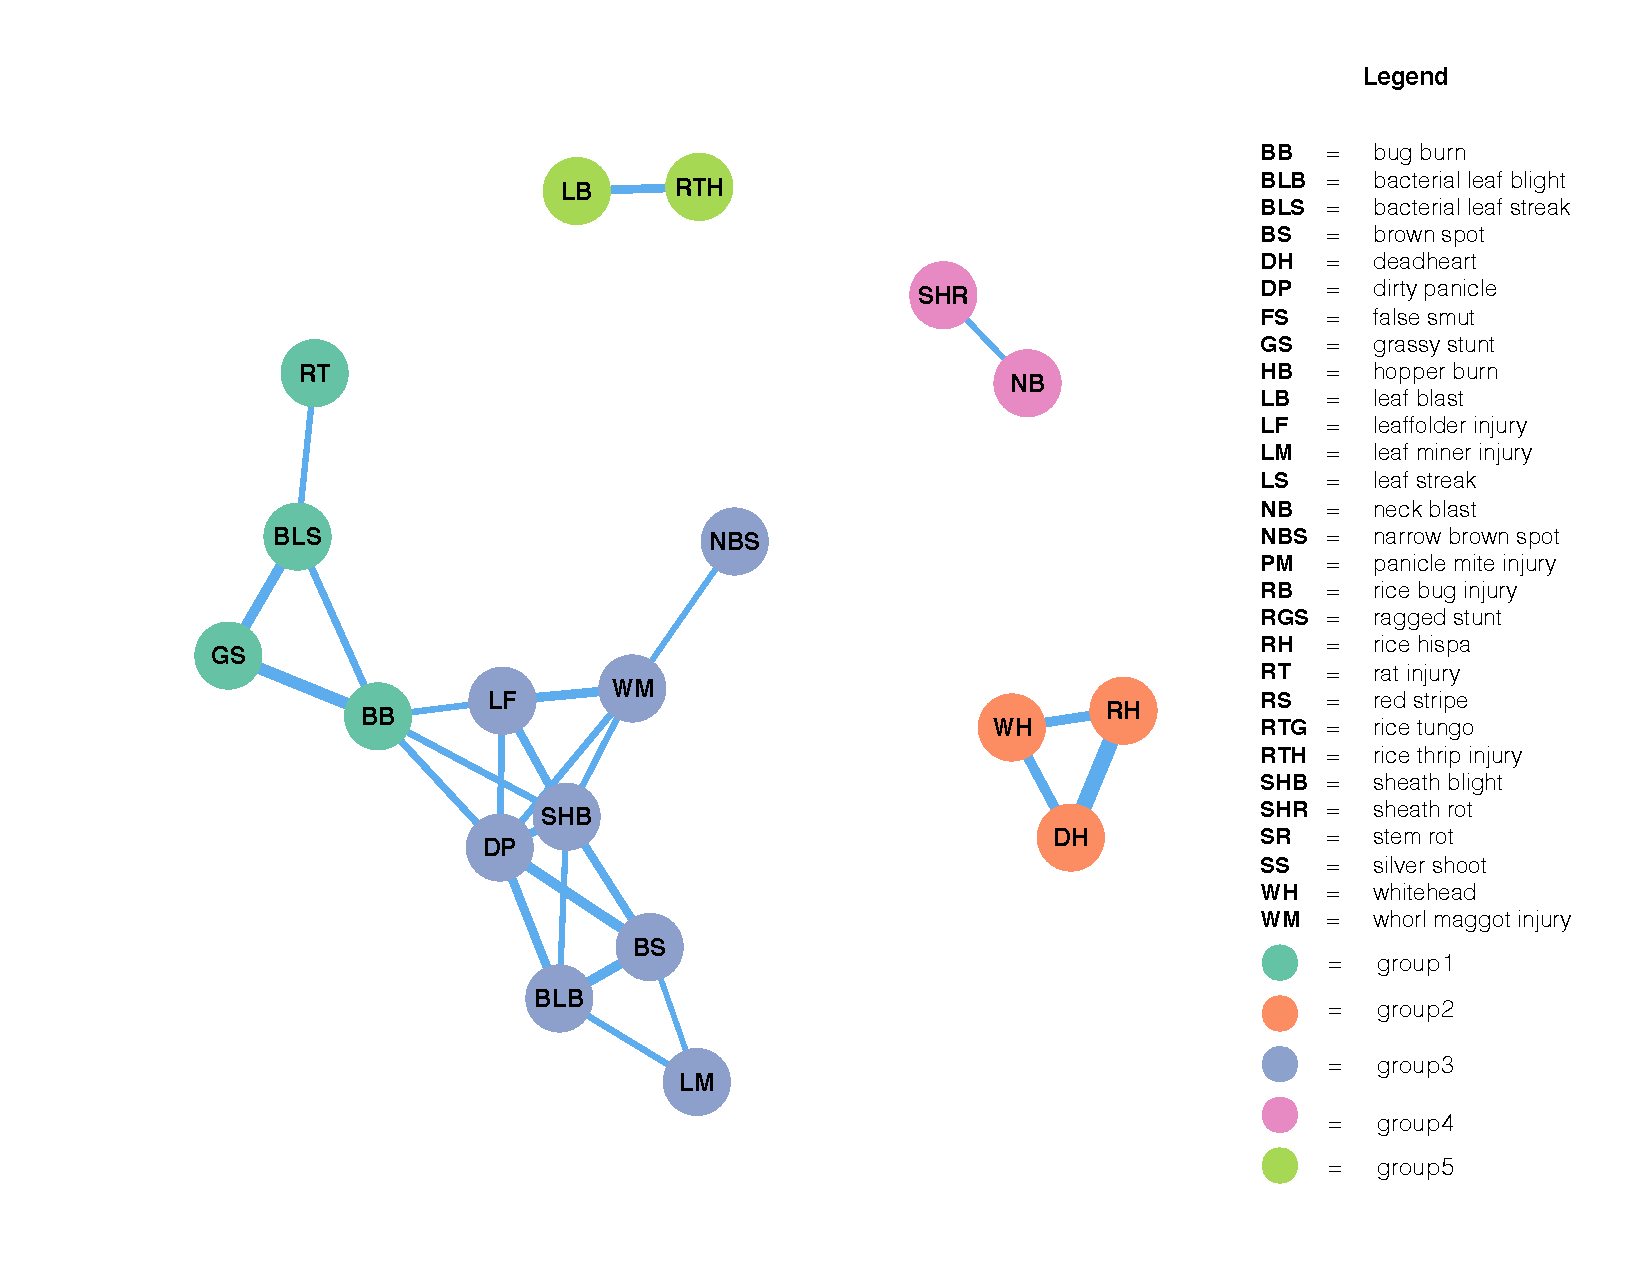
\includegraphics[width = 1\textwidth]{figures/networkRR_ds/networkRR_ds.pdf}
        \caption{Co-occurrence network of rice injuries in dry season at Red River Delta, Vietnam. The layout of the network graph is based on the Fruchterman-Reingold algorithm, which places nodes with stronger or more connections closer to each other.}
        \label{fig:networkRR_ds}
    \end{subfigure}
    \begin{subfigure}[b]{1\textwidth}
        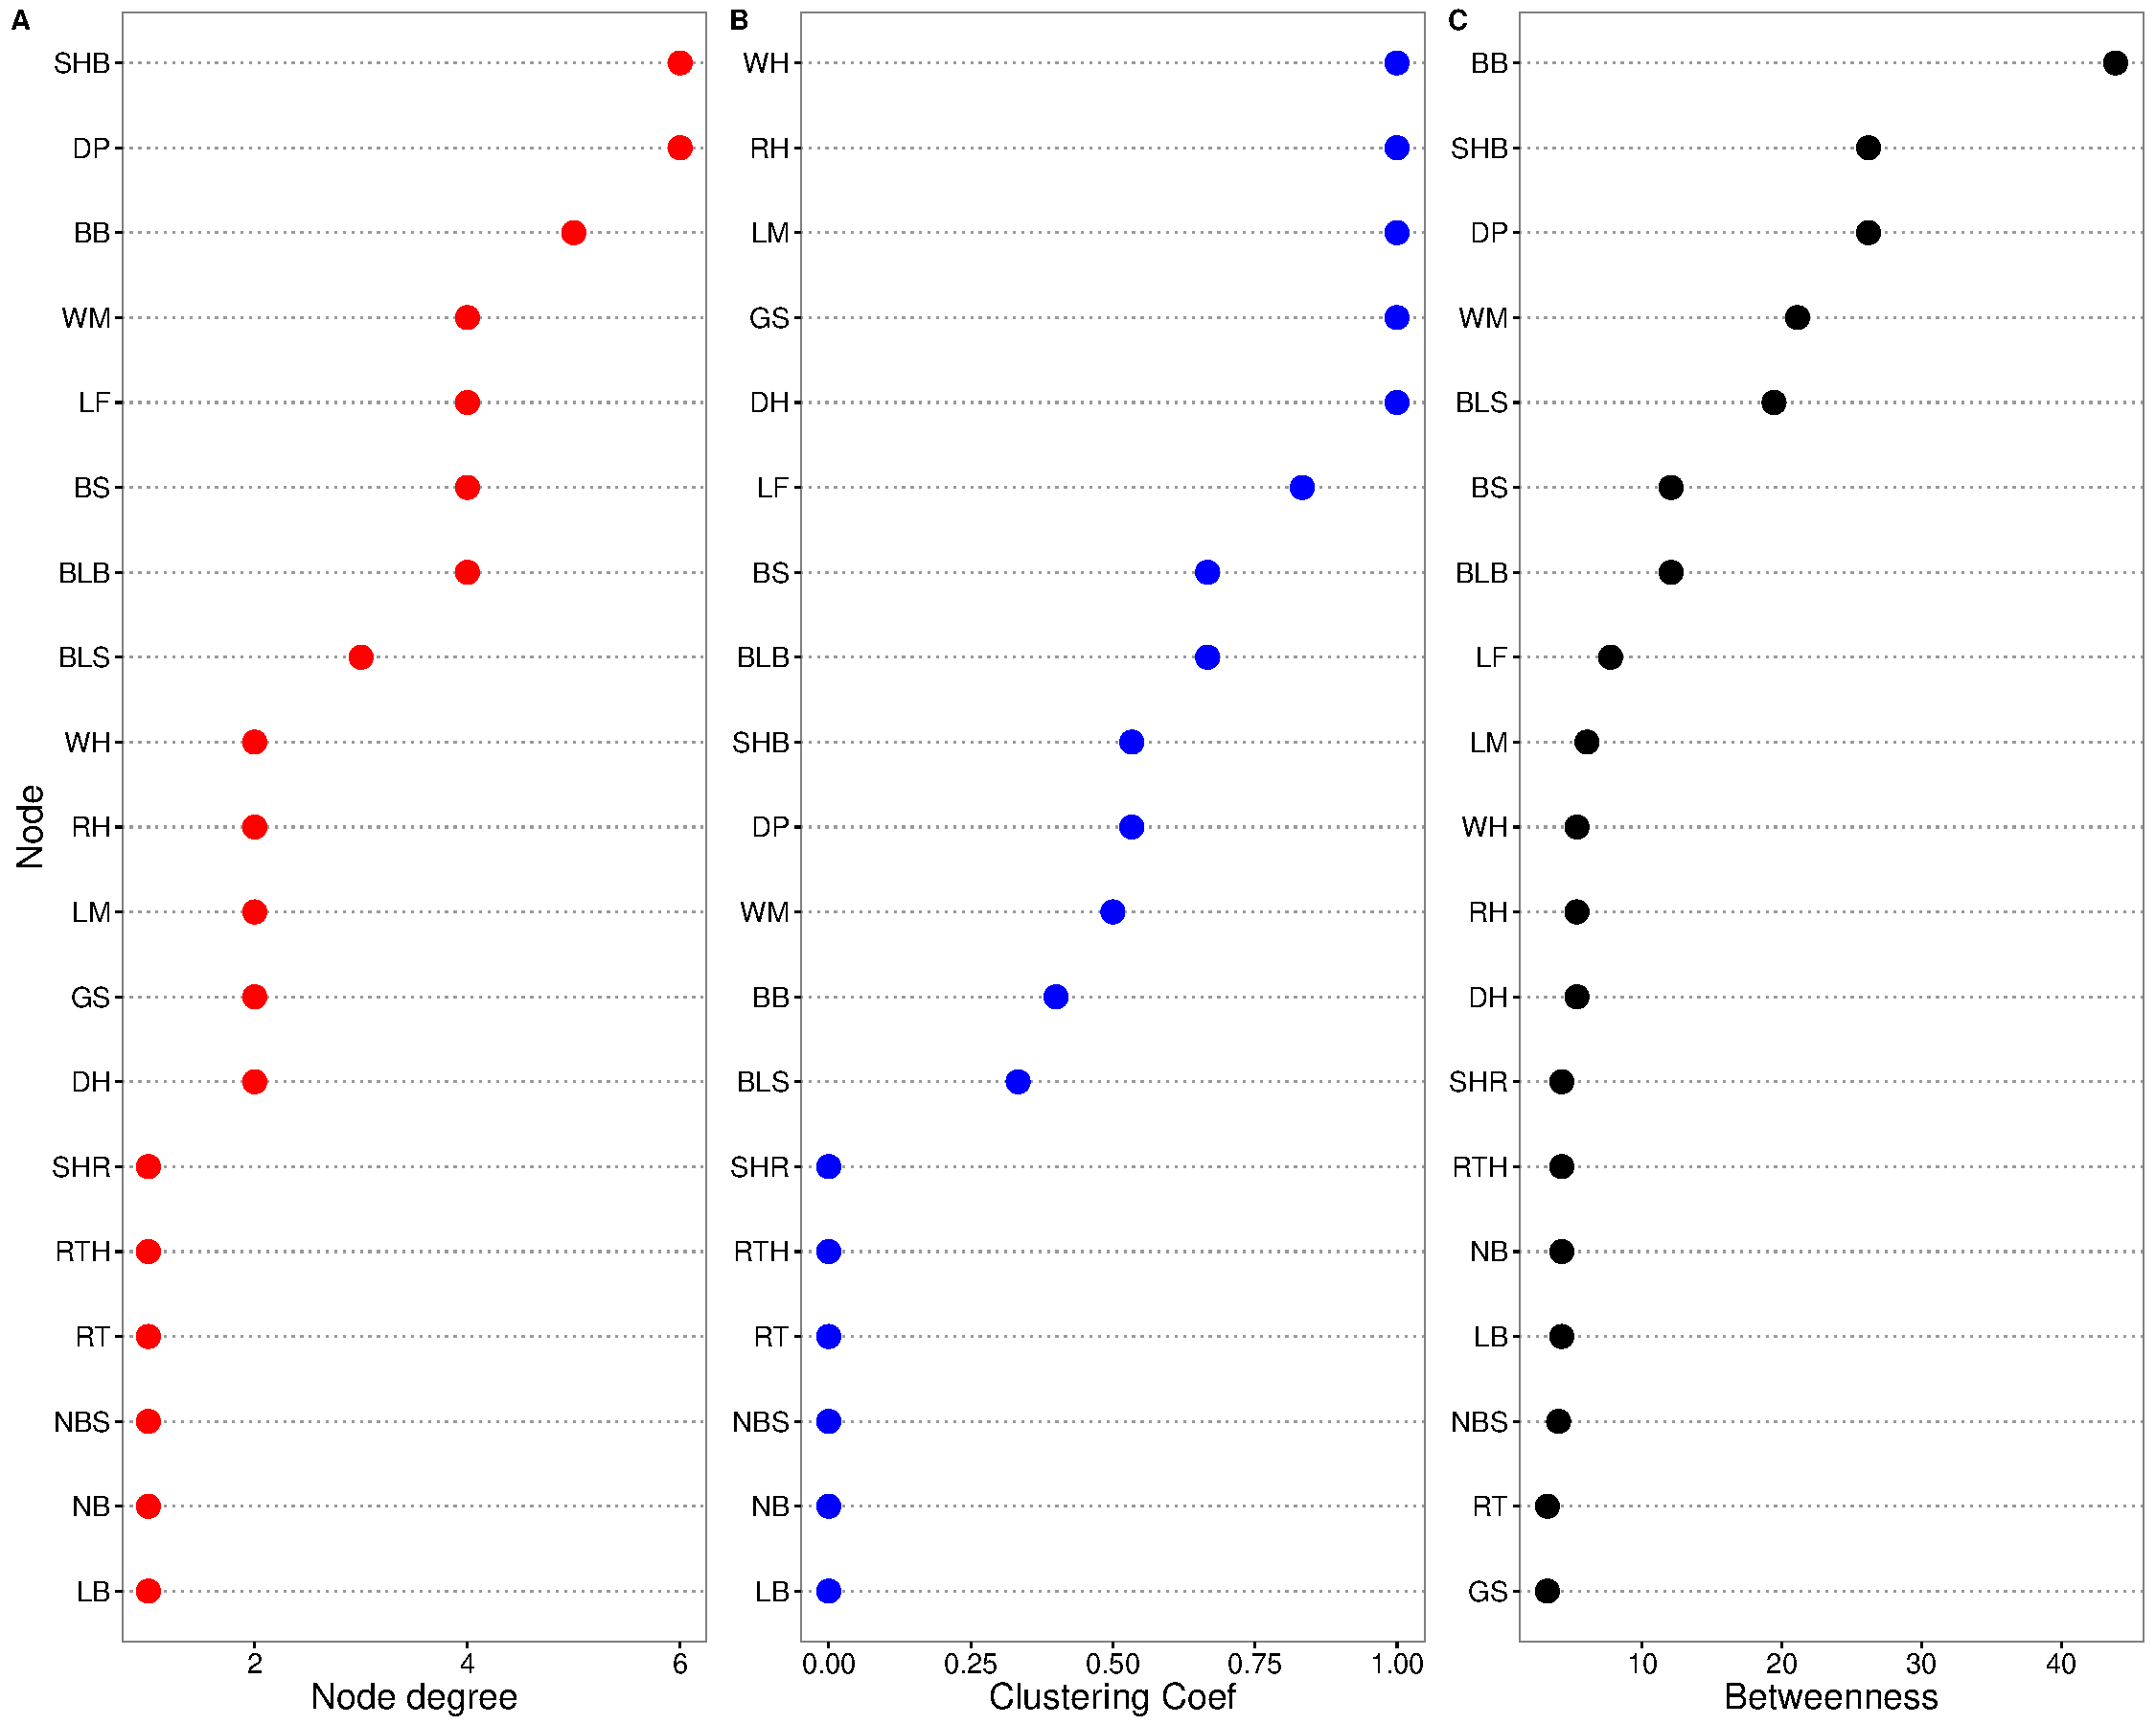
\includegraphics[width = 1\textwidth]{figures/nodepropRR_ds/nodepropRR_ds.pdf}
        \caption{Three centrality measures of the nodes in co-occurrence network of rice injuries in dry season at Red River Delta, Vietnam. A: node degree, B:clustering coefficient, and C:Betweenness}
        \label{fig:nodepropRR_ds}
    \end{subfigure}
    \caption{Rice injuries in dry season in Red River Delta, Vietnam }
    \label{fig:RR_ds}
\end{figure}

\begin{figure}
    \centering
    \begin{subfigure}[b]{1\textwidth}
        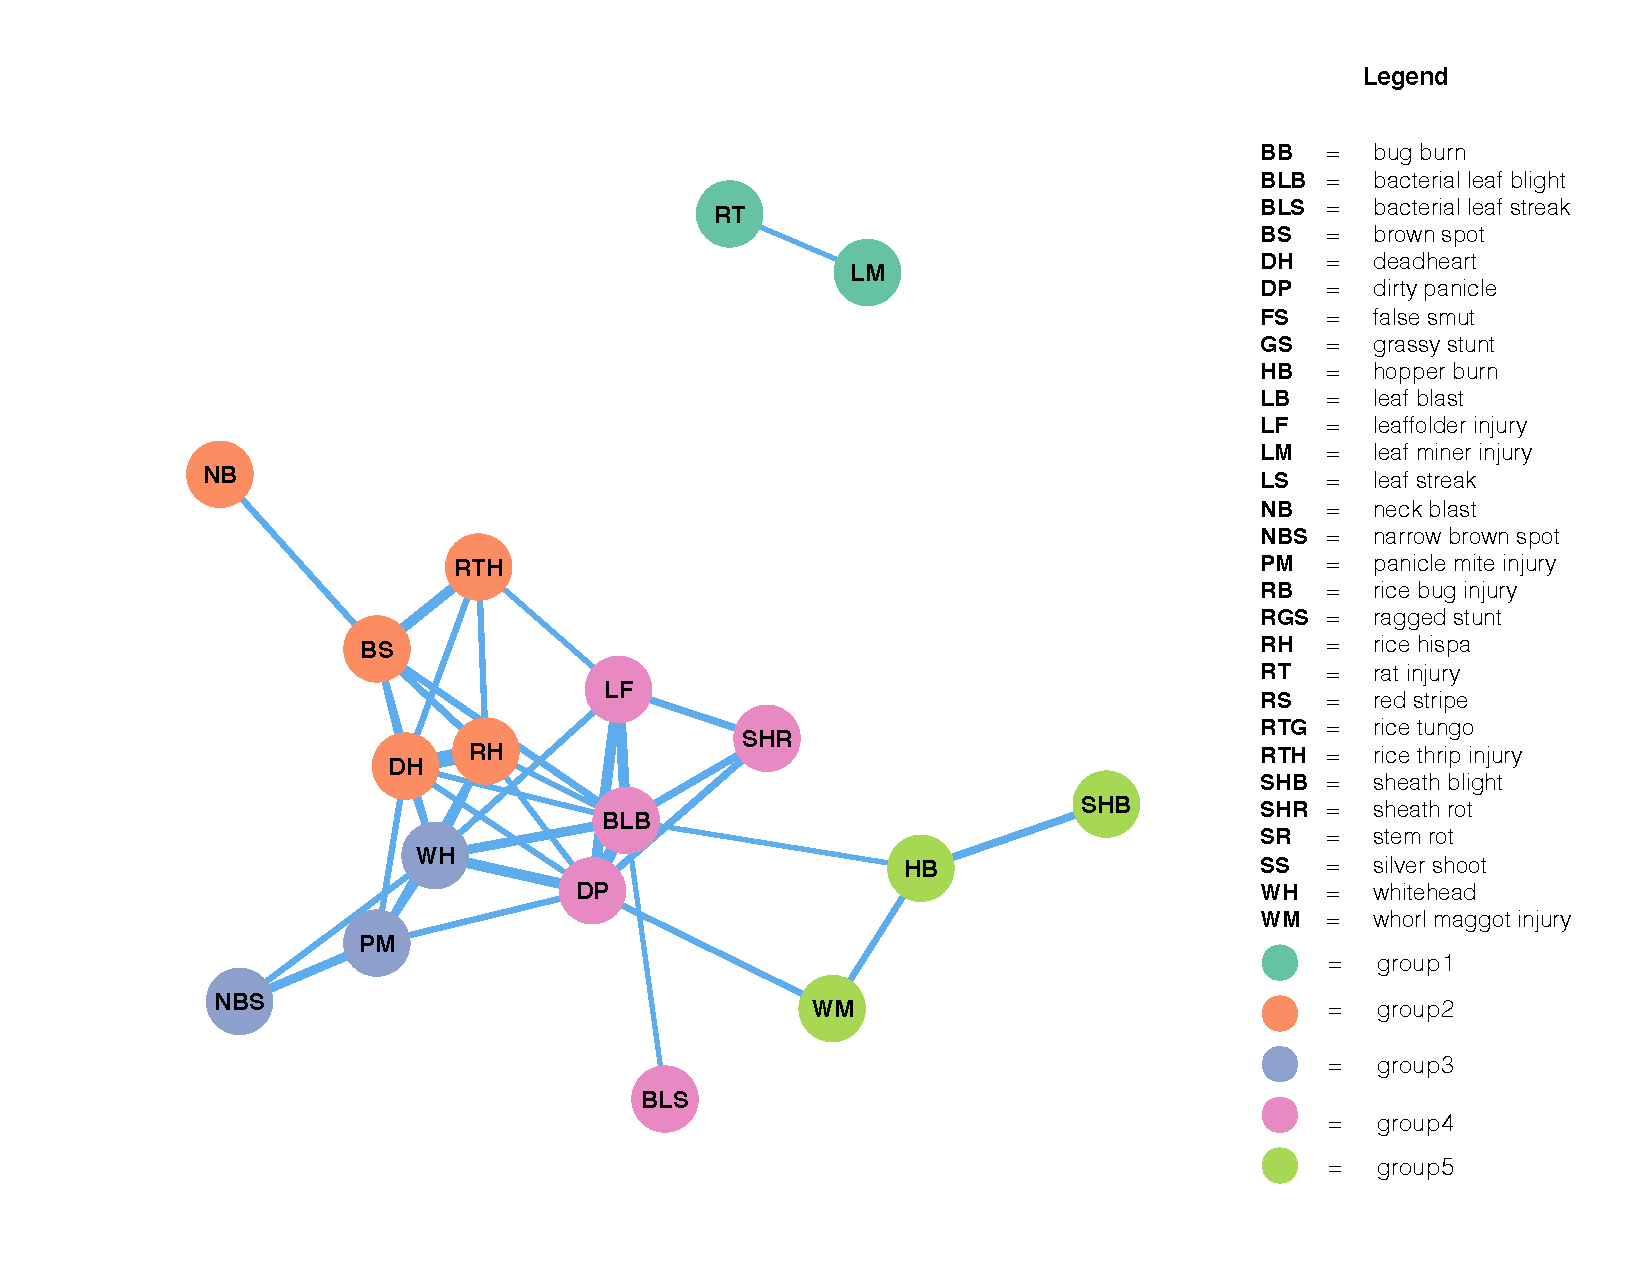
\includegraphics[width = 1\textwidth]{figures/networkRR_ws/networkRR_ws.pdf}
        \caption{Co-occurrence network of rice injuries in wet season at Red River Delta, Vietnam. The layout of the network graph is based on the Fruchterman-Reingold algorithm, which places nodes with stronger or more connections closer to each other.}
        \label{fig:networkRR_ws}
    \end{subfigure}
    \begin{subfigure}[b]{1\textwidth}
        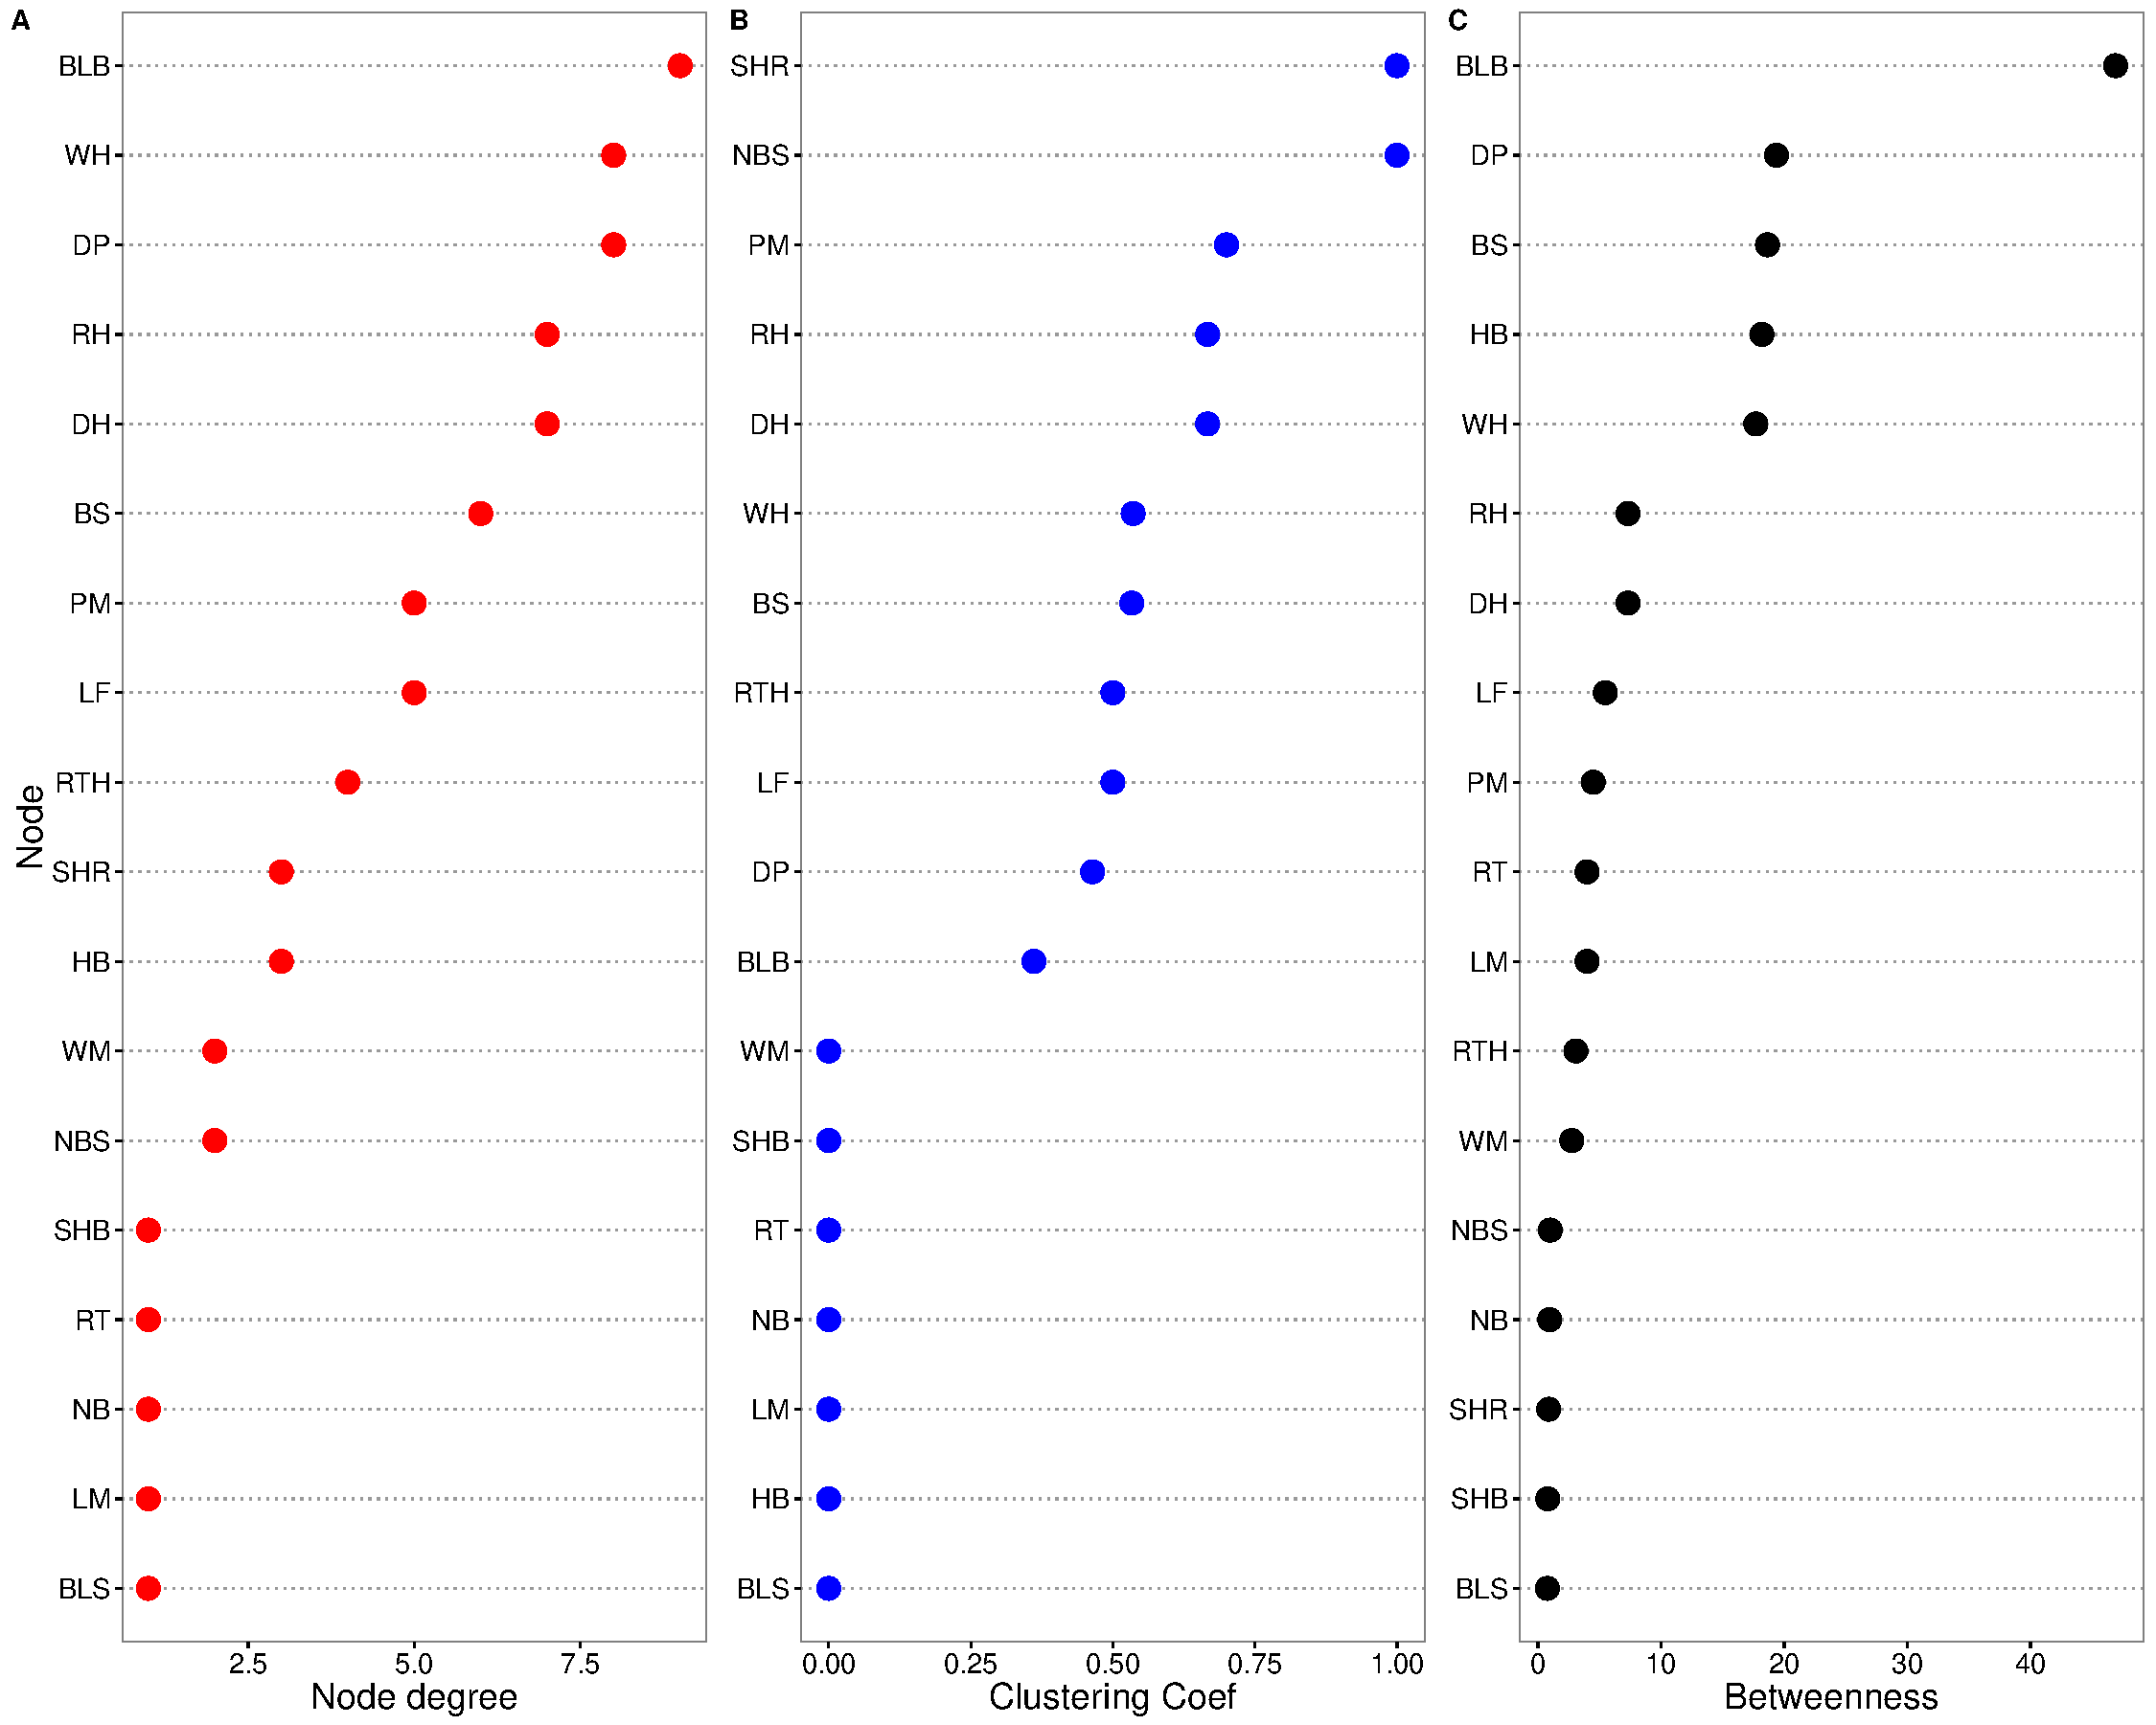
\includegraphics[width = 1\textwidth]{figures/nodepropRR_ws/nodepropRR_ws.pdf}
        \caption{Three centrality measures of the nodes in co-occurrence network of rice injuries in wet season at Red River Delta, Vietnam. A: node degree, B:clustering coefficient, and C:Betweenness}
        \label{fig:nodepropRR_ws}
    \end{subfigure}
    \caption{Rice injuries in wet season in Red River Delta, Vietnam}
    \label{fig:RR_ws}
\end{figure}


\paragraph{Tamil Nadu, India}

The dry season network (Fig \ref{fig:networkTM_ds}) revealed three clustered groups of injury profiles. One of them was separated from other two. Group1 was condensed, which differ from group2 that injuries were placed further. SHB and BLB were disconnected to the rest.  BS and WH highly tended to occur in this season (high betweenness).  Because clustering coefficient value of members in group2 less than group1, injuries in group2 might occur together with one or two more injuries. But in group1, the combination was more complex than. 16 node, and 31 relationships

Figure \ref{fig:networkTM_ws} presented co-occurrence network of injury profiles in dry season. Network resulted three groups of injury profiles. Compared to other groups, group3 had less connection. Group1 had high node degree injuries. 12 node 30 relationships


\begin{figure}
    \centering
    \begin{subfigure}[b]{1\textwidth}
        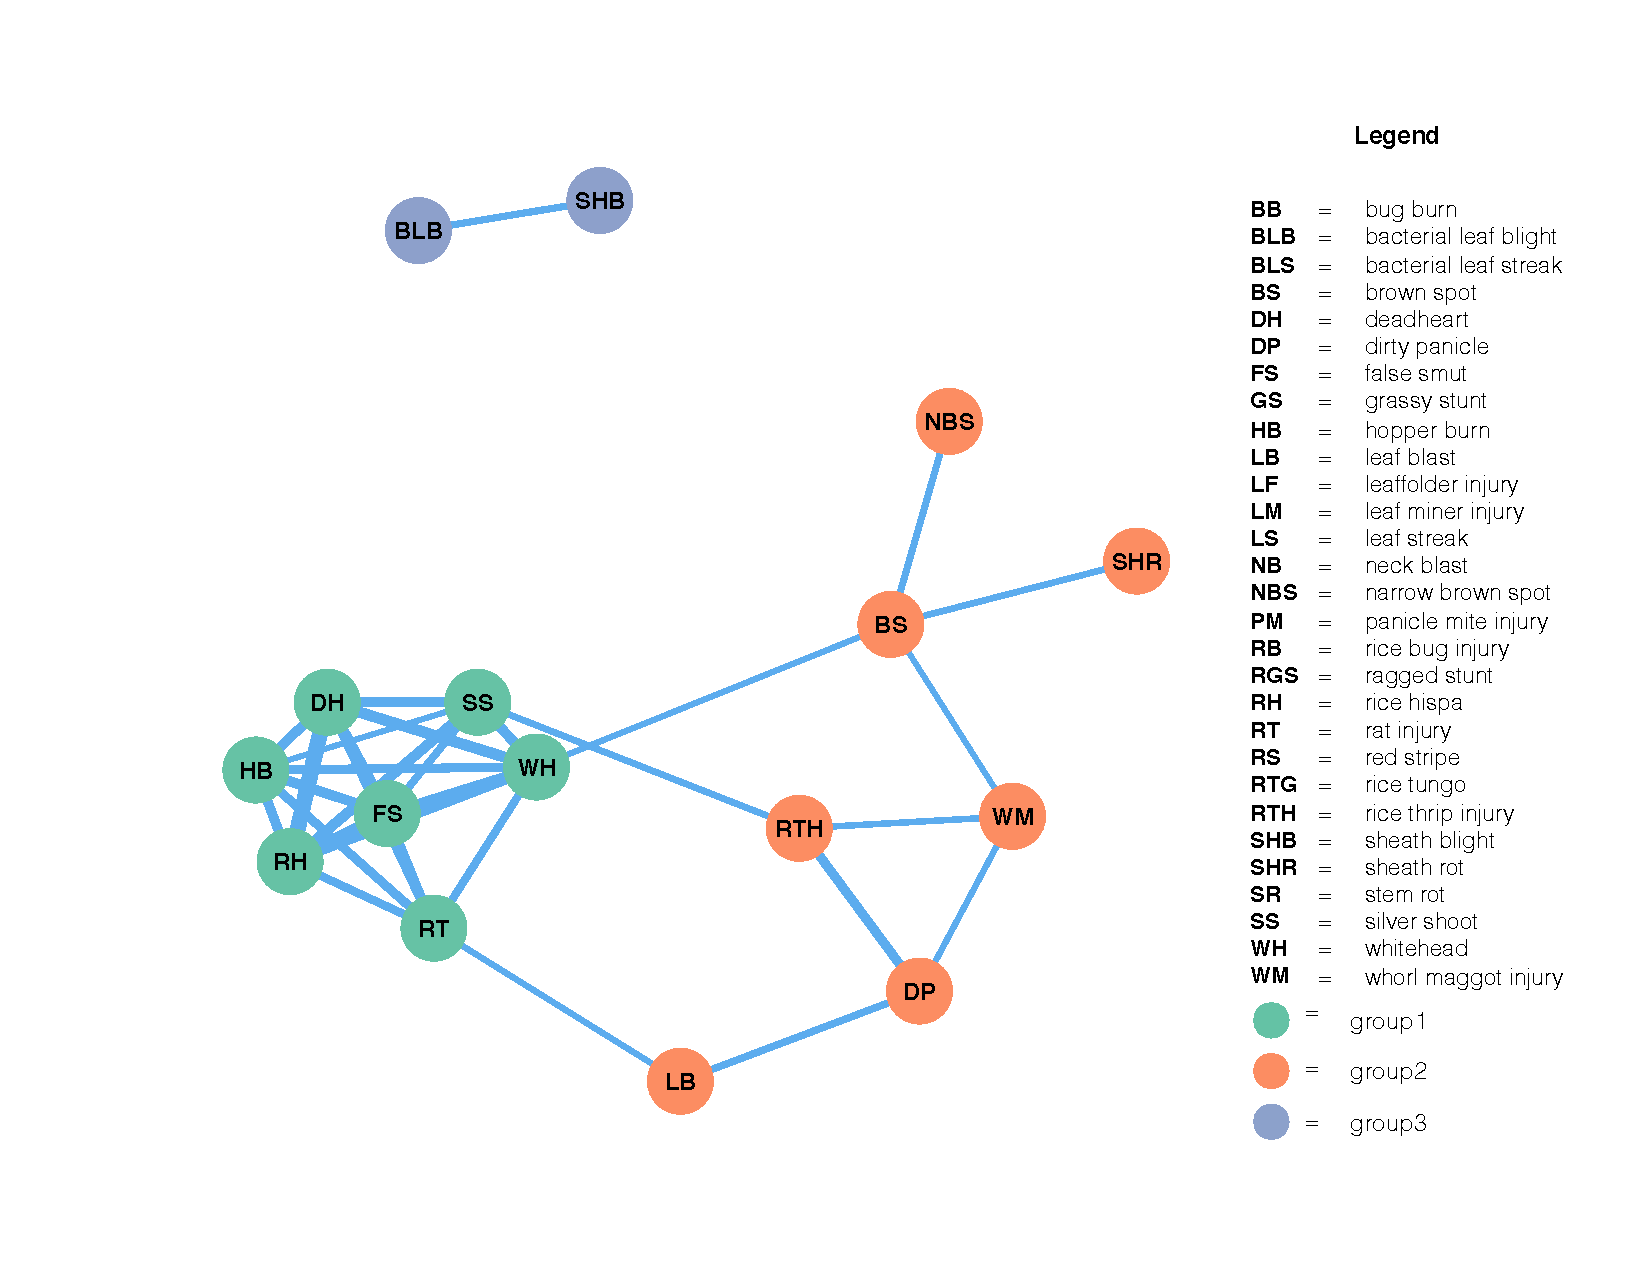
\includegraphics[width = 1\textwidth]{figures/networkTM_ds/networkTM_ds.pdf}
        \caption{Co-occurrence network of rice injuries in dry season at Tamil Nadu, India. The layout of the network graph is based on the Fruchterman-Reingold algorithm, which places nodes with stronger or more connections closer to each other.}
        \label{fig:networkTM_ds}
    \end{subfigure}
    \begin{subfigure}[b]{1\textwidth}
        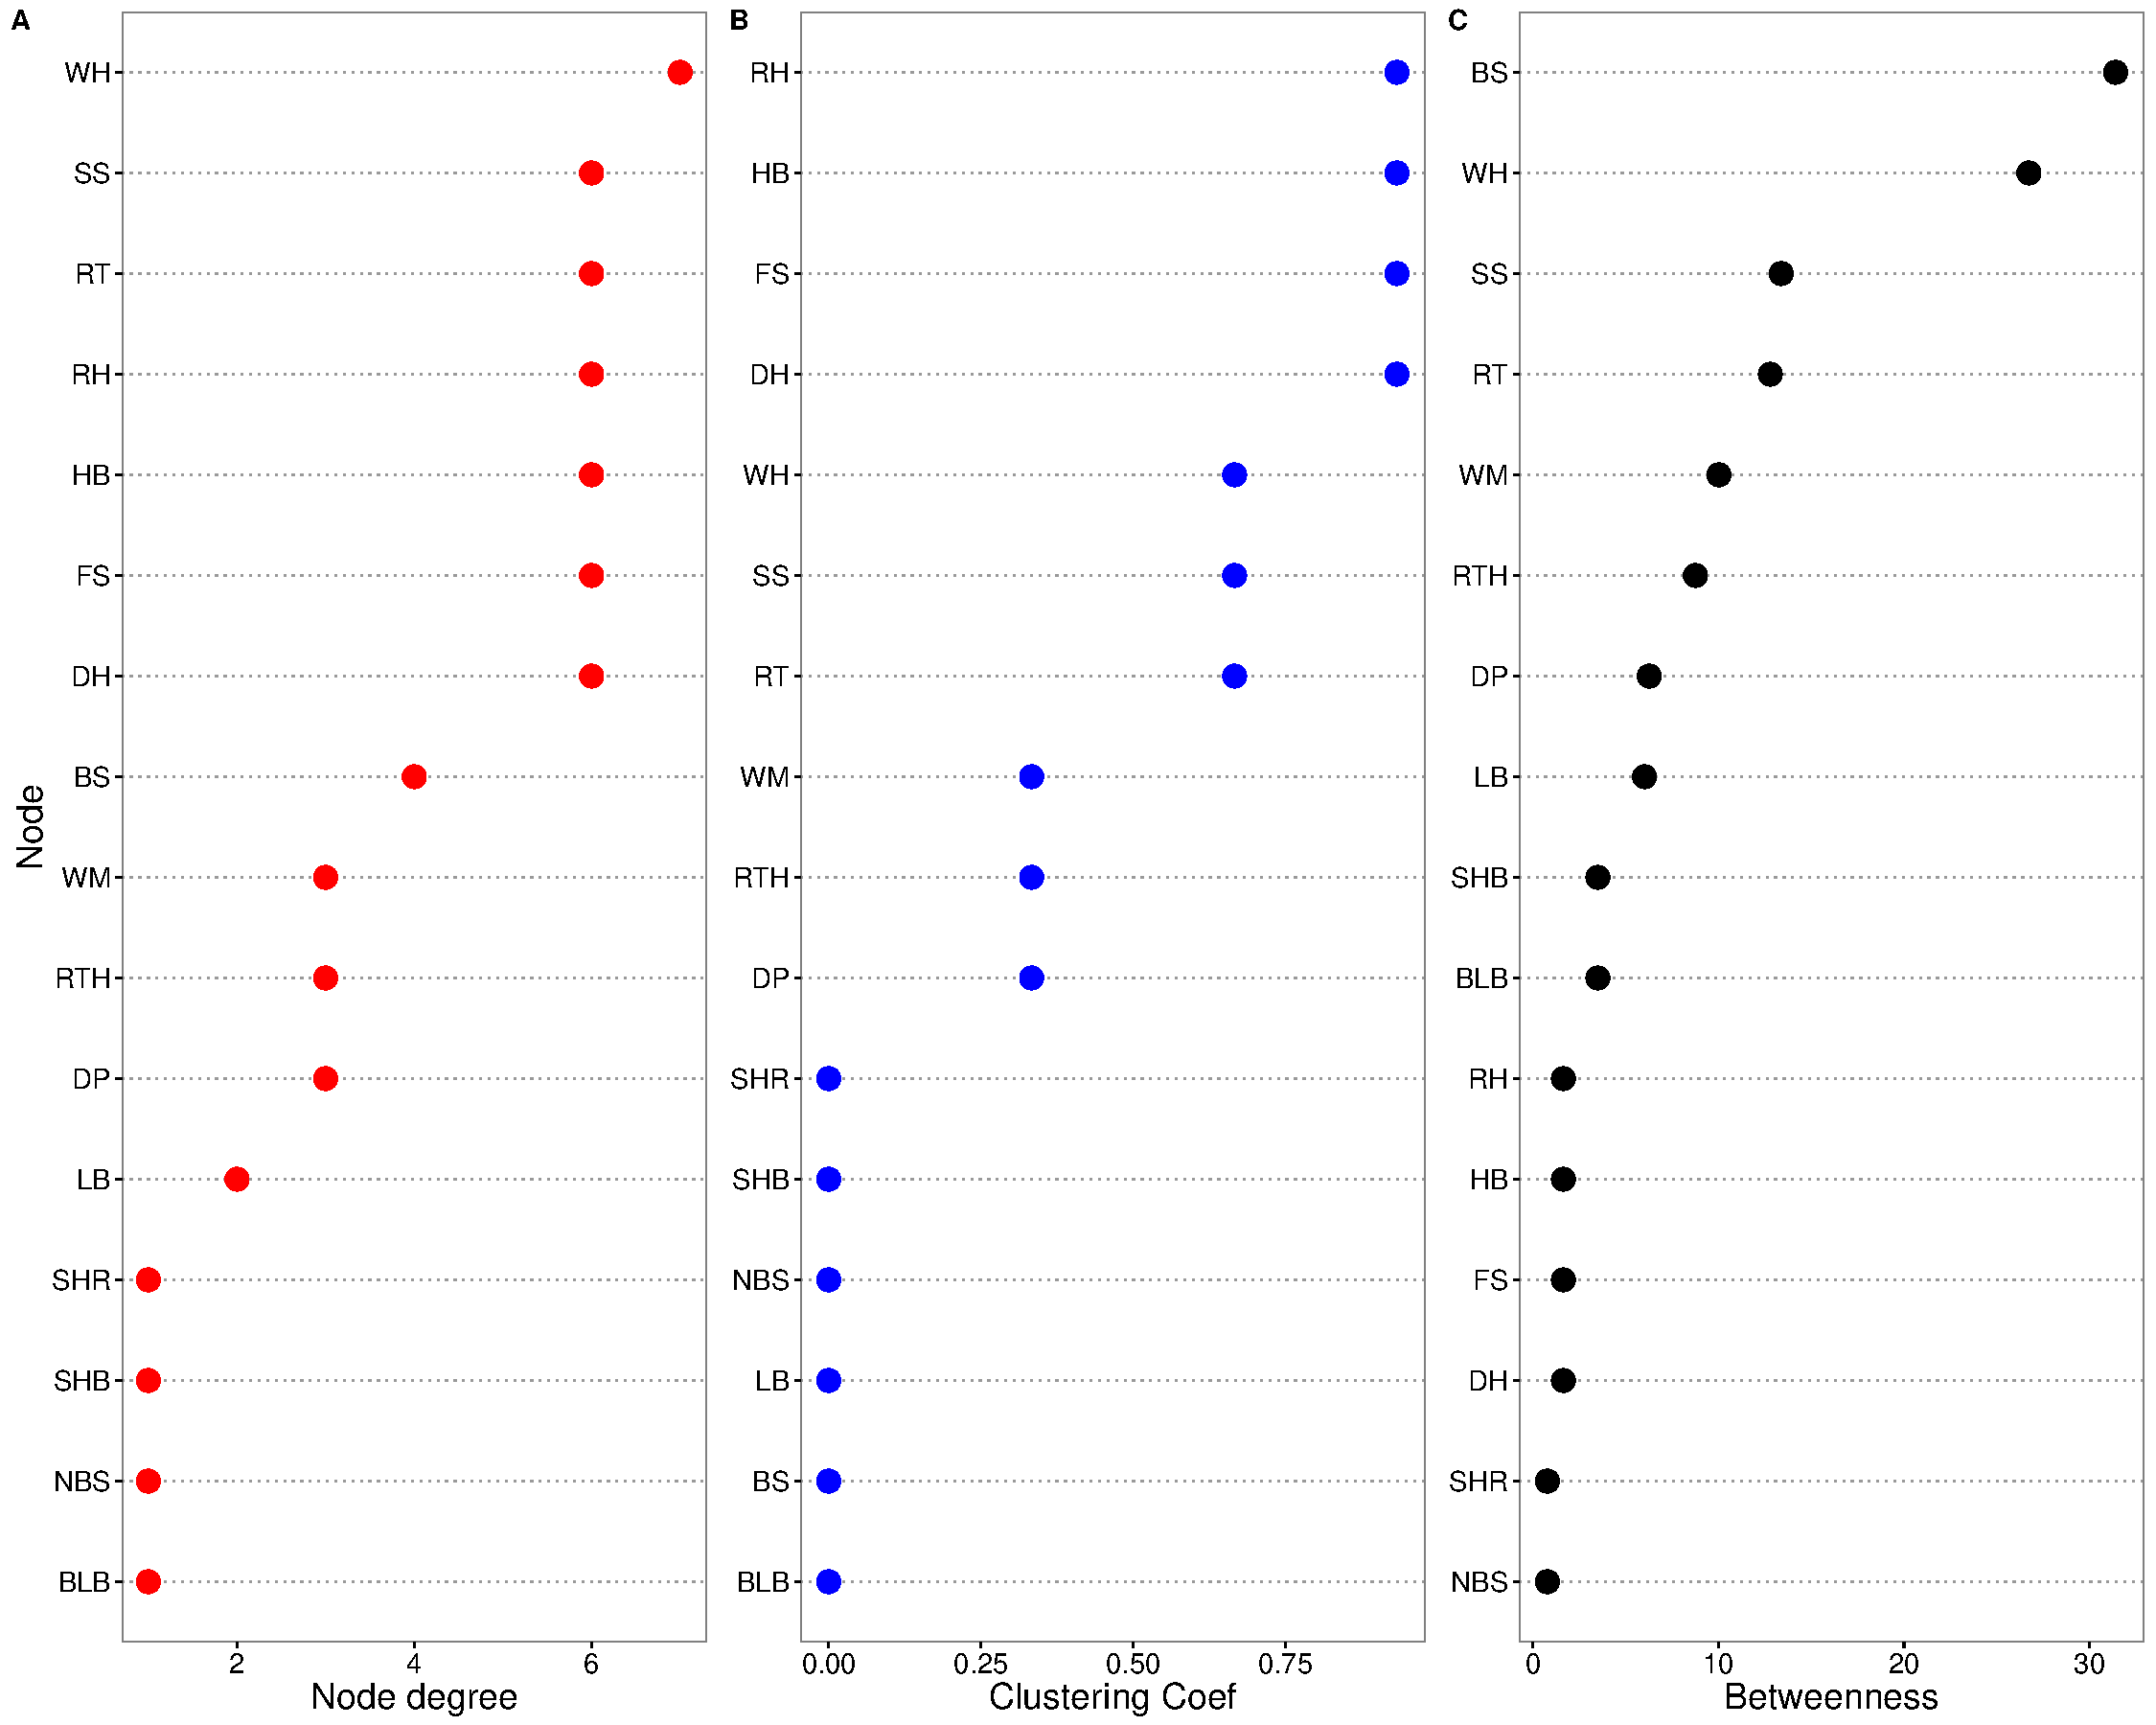
\includegraphics[width = 1\textwidth]{figures/nodepropTM_ds/nodepropTM_ds.pdf}
        \caption{Three centrality measures of the nodes in co-occurrence network of rice injuries in dry season at Tamil Nadu, India. A: node degree, B:clustering coefficient, and C:Betweenness.}
        \label{fig:nodepropTM_ds}
    \end{subfigure}
    \caption{Rice injuries in dry season in Tamil Nadu, India}
    \label{fig:TM_ds}
\end{figure}

\begin{figure}
    \centering
    \begin{subfigure}[b]{1\textwidth}
        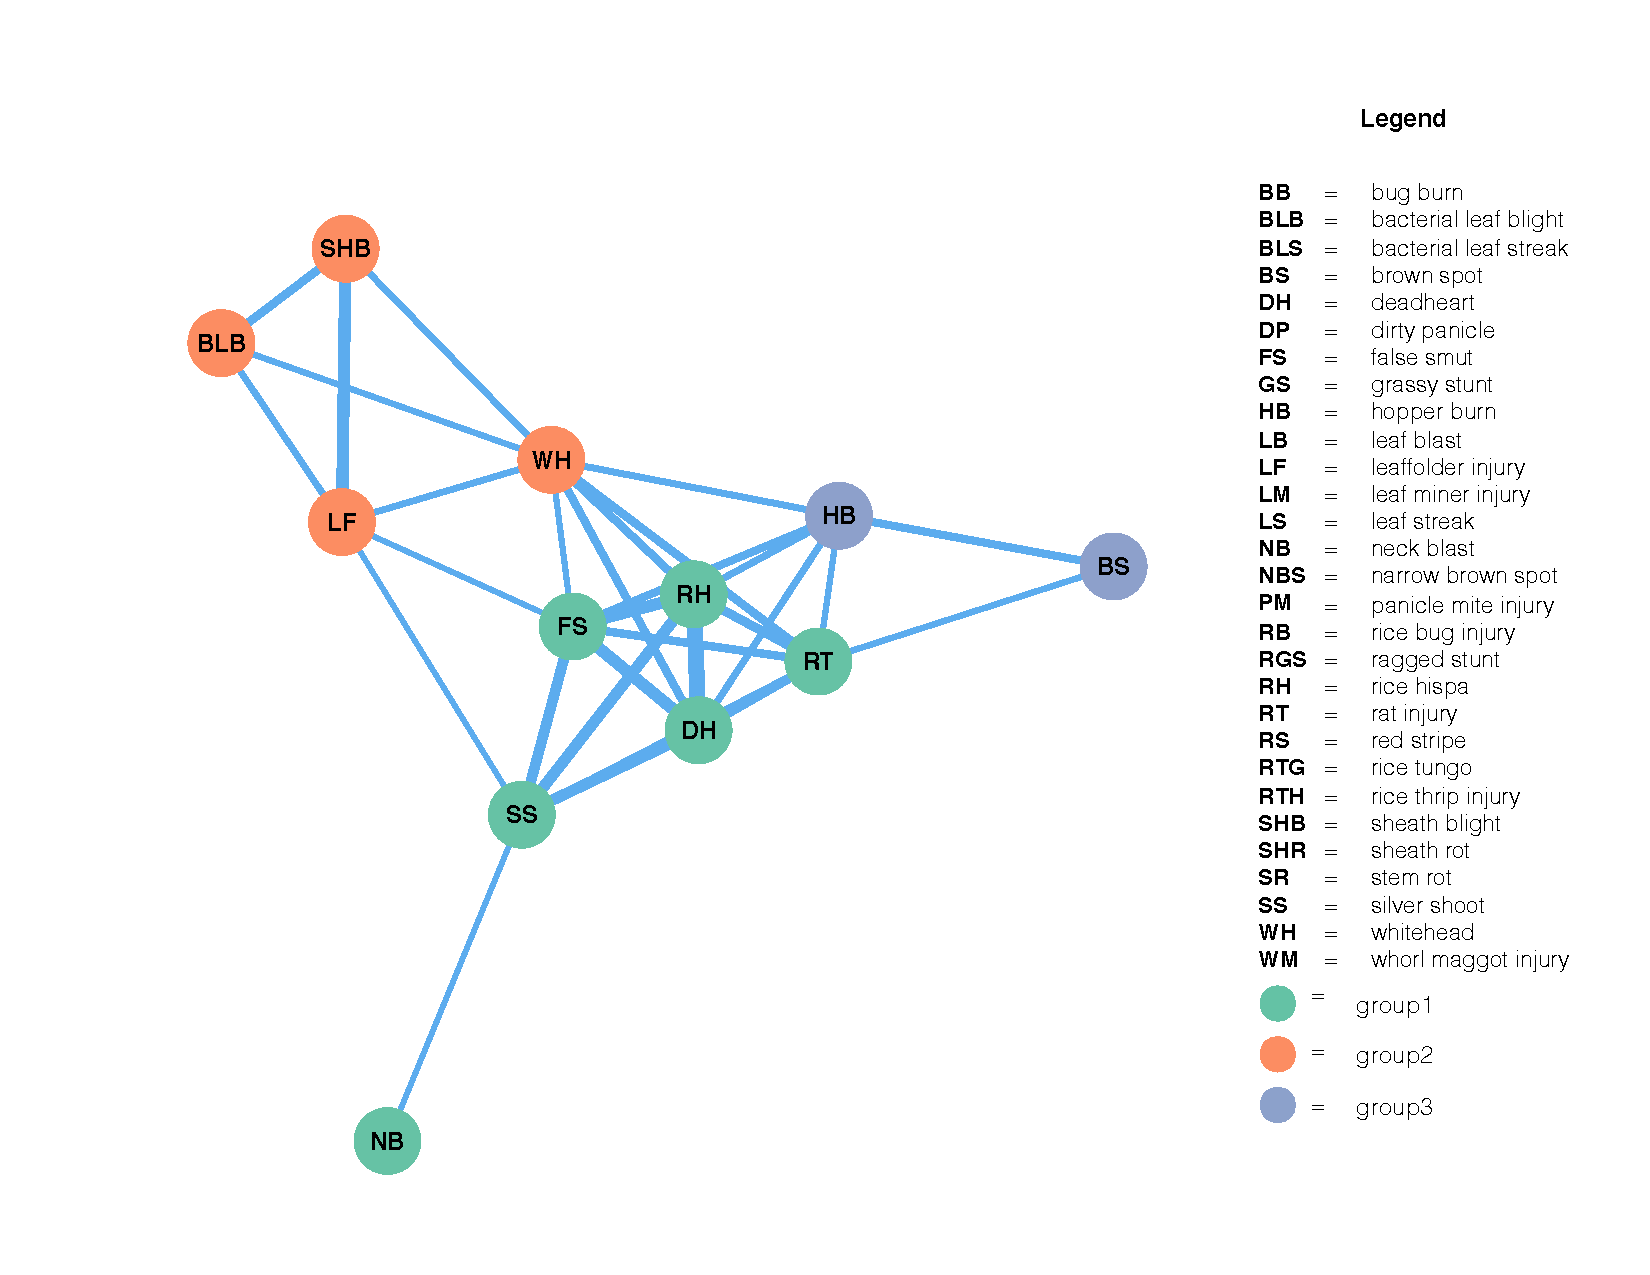
\includegraphics[width = 1\textwidth]{figures/networkTM_ws/networkTM_ws.pdf}
        \caption{Co-occurrence network of rice injuries in wet season at Tamil Nadu, India. The layout of the network graph is based on the Fruchterman-Reingold algorithm, which places nodes with stronger or more connections closer to each other.}
        \label{fig:networkTM_ws}
    \end{subfigure}
    \begin{subfigure}[b]{1\textwidth}
        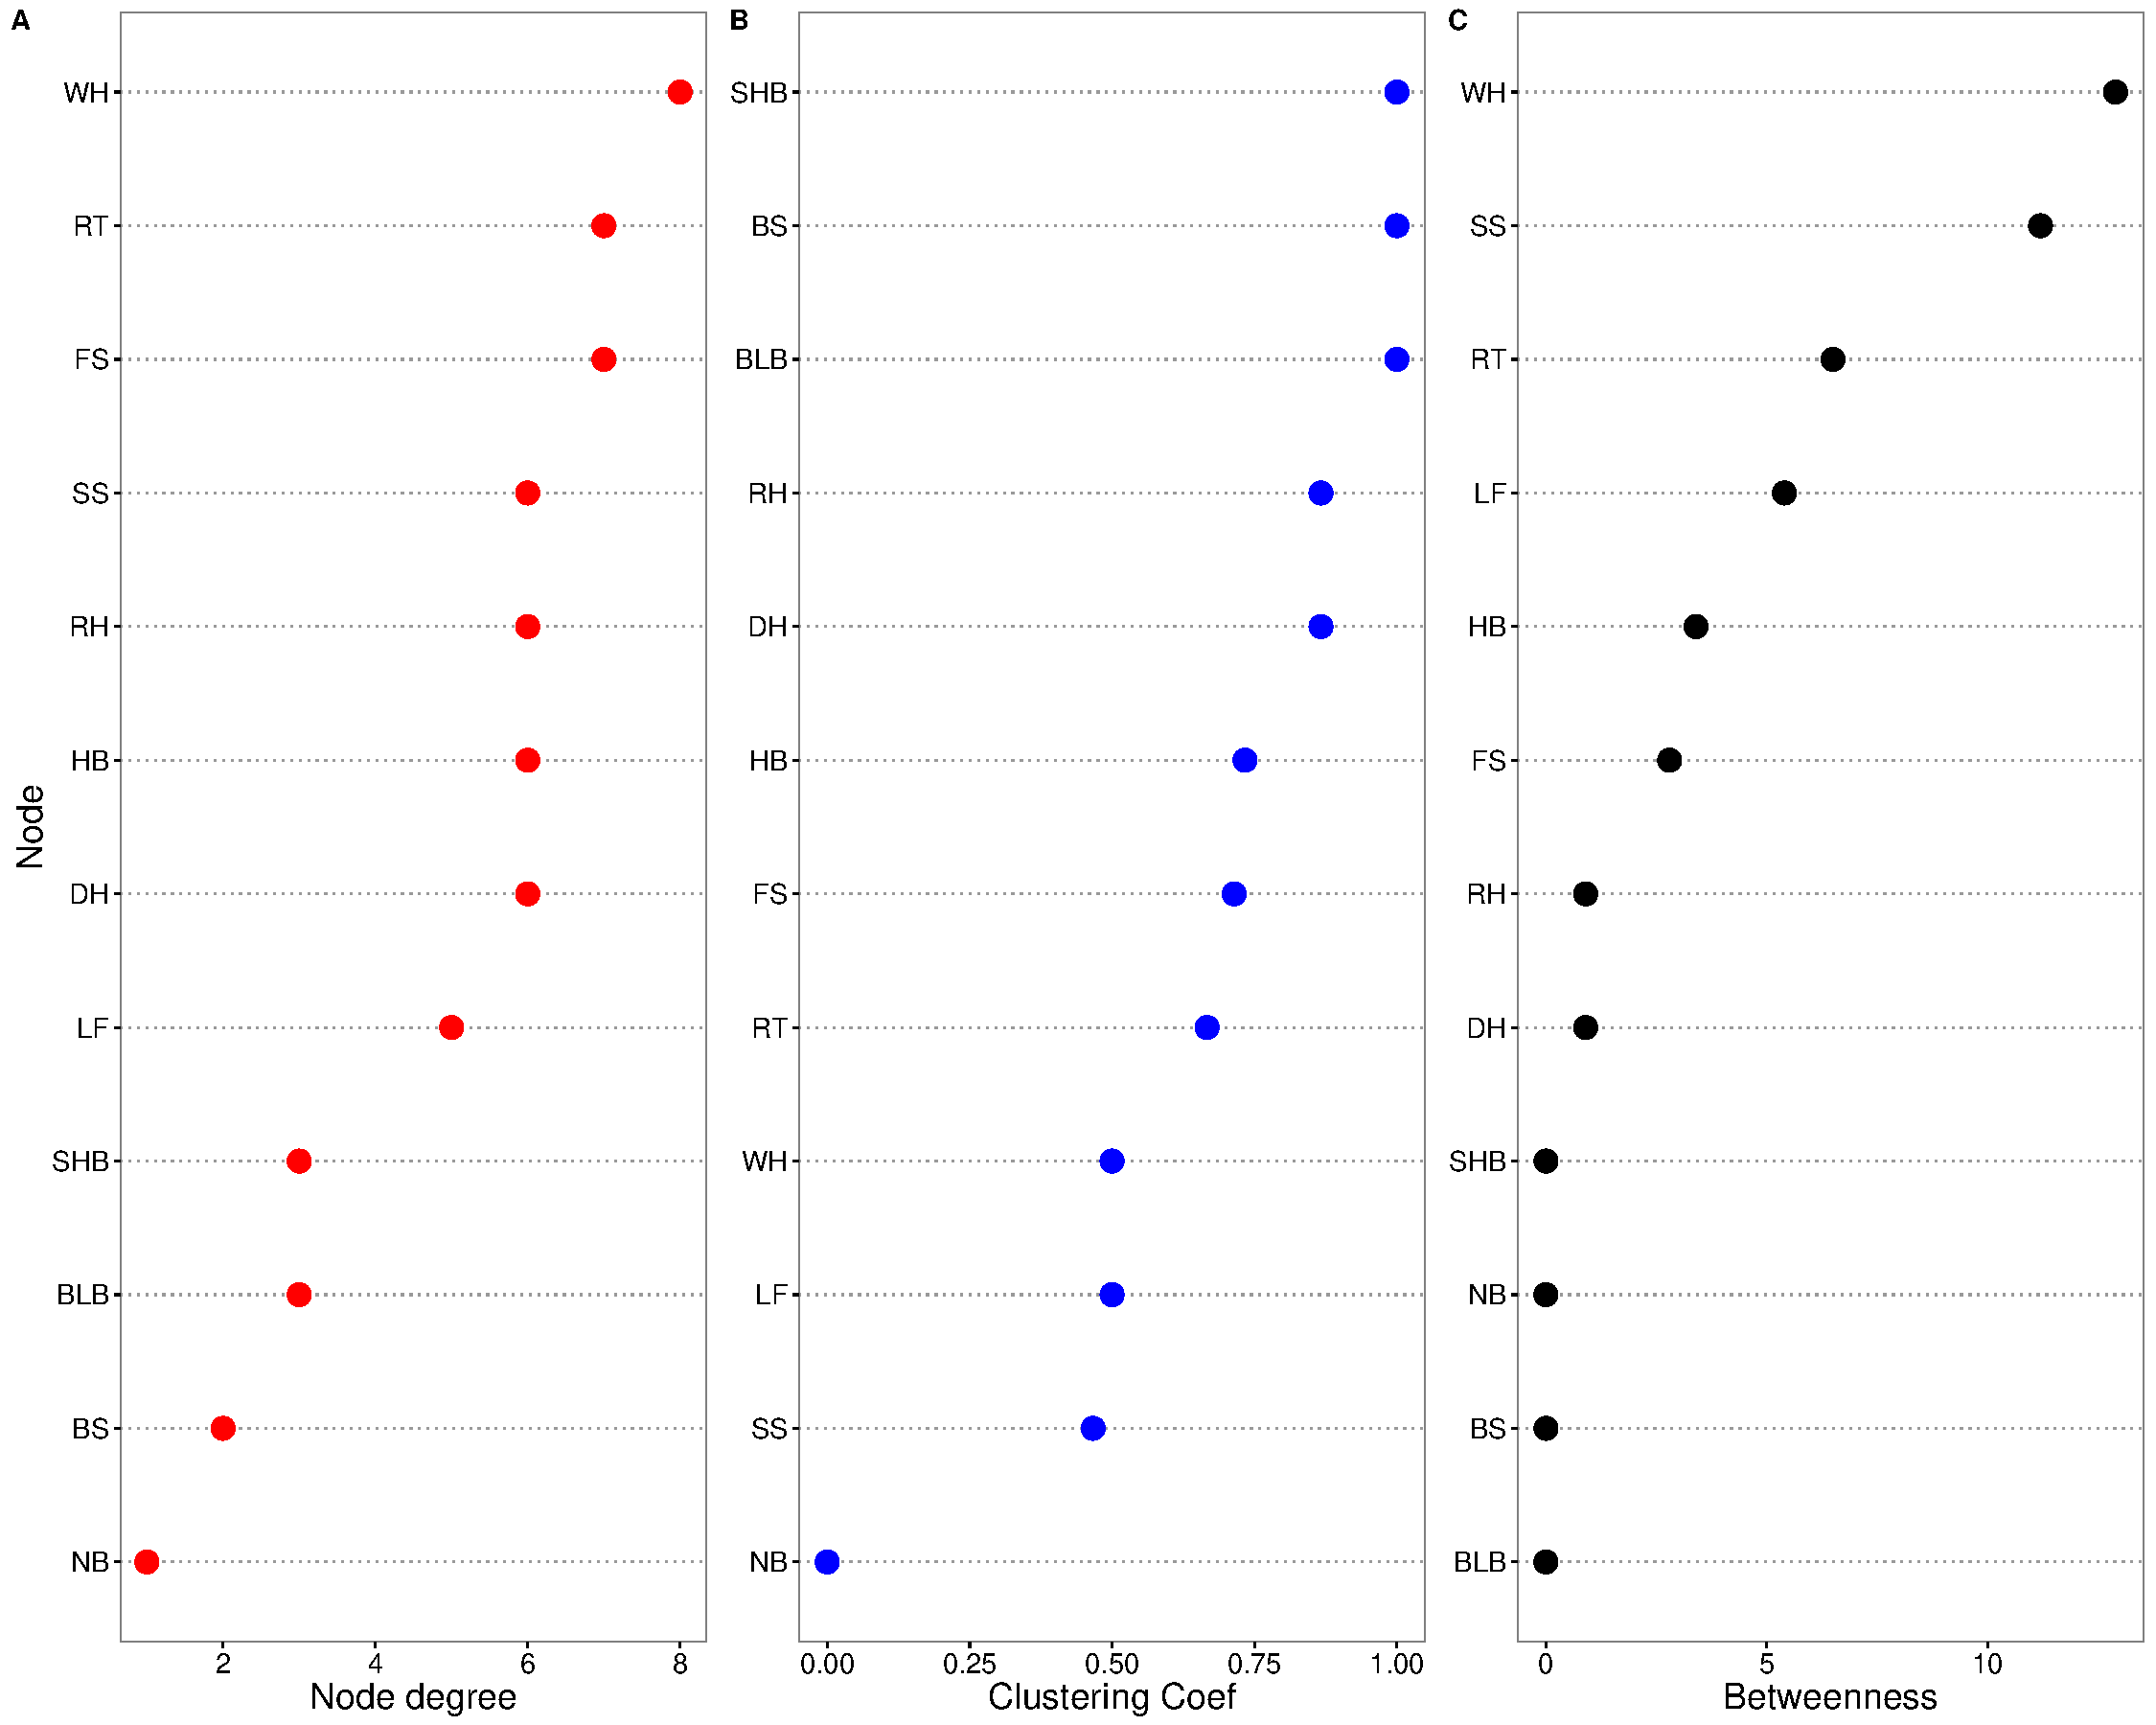
\includegraphics[width = 1\textwidth]{figures/nodepropTM_ws/nodepropTM_ws.pdf}
        \caption{Three centrality measures of the nodes in co-occurrence network of rice injuries in wet season at Tamil Nadu, India. A: node degree, B:clustering coefficient, and C:Betweenness.}
        \label{fig:nodepropTM_ws}
    \end{subfigure}
    \caption{Rice injuries in wet season in Tamil Nadu, India}
    \label{fig:TM_ws}
\end{figure}

\paragraph{West Java, Indonesia}

Co-occurrence network of injury profiles of dry season presented in Figure \ref{fig:networkWJ_ds} showing 26 injury nodes and 99 association. Huge number of pest injuries and disease could be observes in dry season.  The network reveals the four groups of injury profiles. Group1 (green) and group3 were close and group2 and group4 had less connection than others. Because of the structure and clustering coefficient, group1 and group3 are more likely to have chance to form complex association to each other. DH and RH of group2 only related to BB of group1 and BS of group3 but not to any of group4. RT has smallest vales of all centrality measures. It indicated RT incidence is independent to other injuries.    

The co-occurrence network of injuries of wet season (Figure \ref{fig:networkWJ_ws}) shows 14 injuries and 18 associations. Compared to the network of dry season the numbers of pest injuries and diseases in wet season are less. The network structure reveals three types of injury syndromes. Group1 (green) composed of SHB, RT, DH, RH, BLS, and SHR.  Within this group, BLS seems to be inducers (high betweenness), and SHB was connecter (high node degree). Group2 (orange) seems to be the group of injuries at panicle level because there is the combination of PM, RB, and FS. Apparently, within this combination, BS is center of association, and early occur among other injuries. Group3 (purple) is combination of BS, LF, WM, NBS, and LM. All of injuries in this group are leaf injuries. 

\begin{figure}
    \centering
    \begin{subfigure}[b]{1\textwidth}
        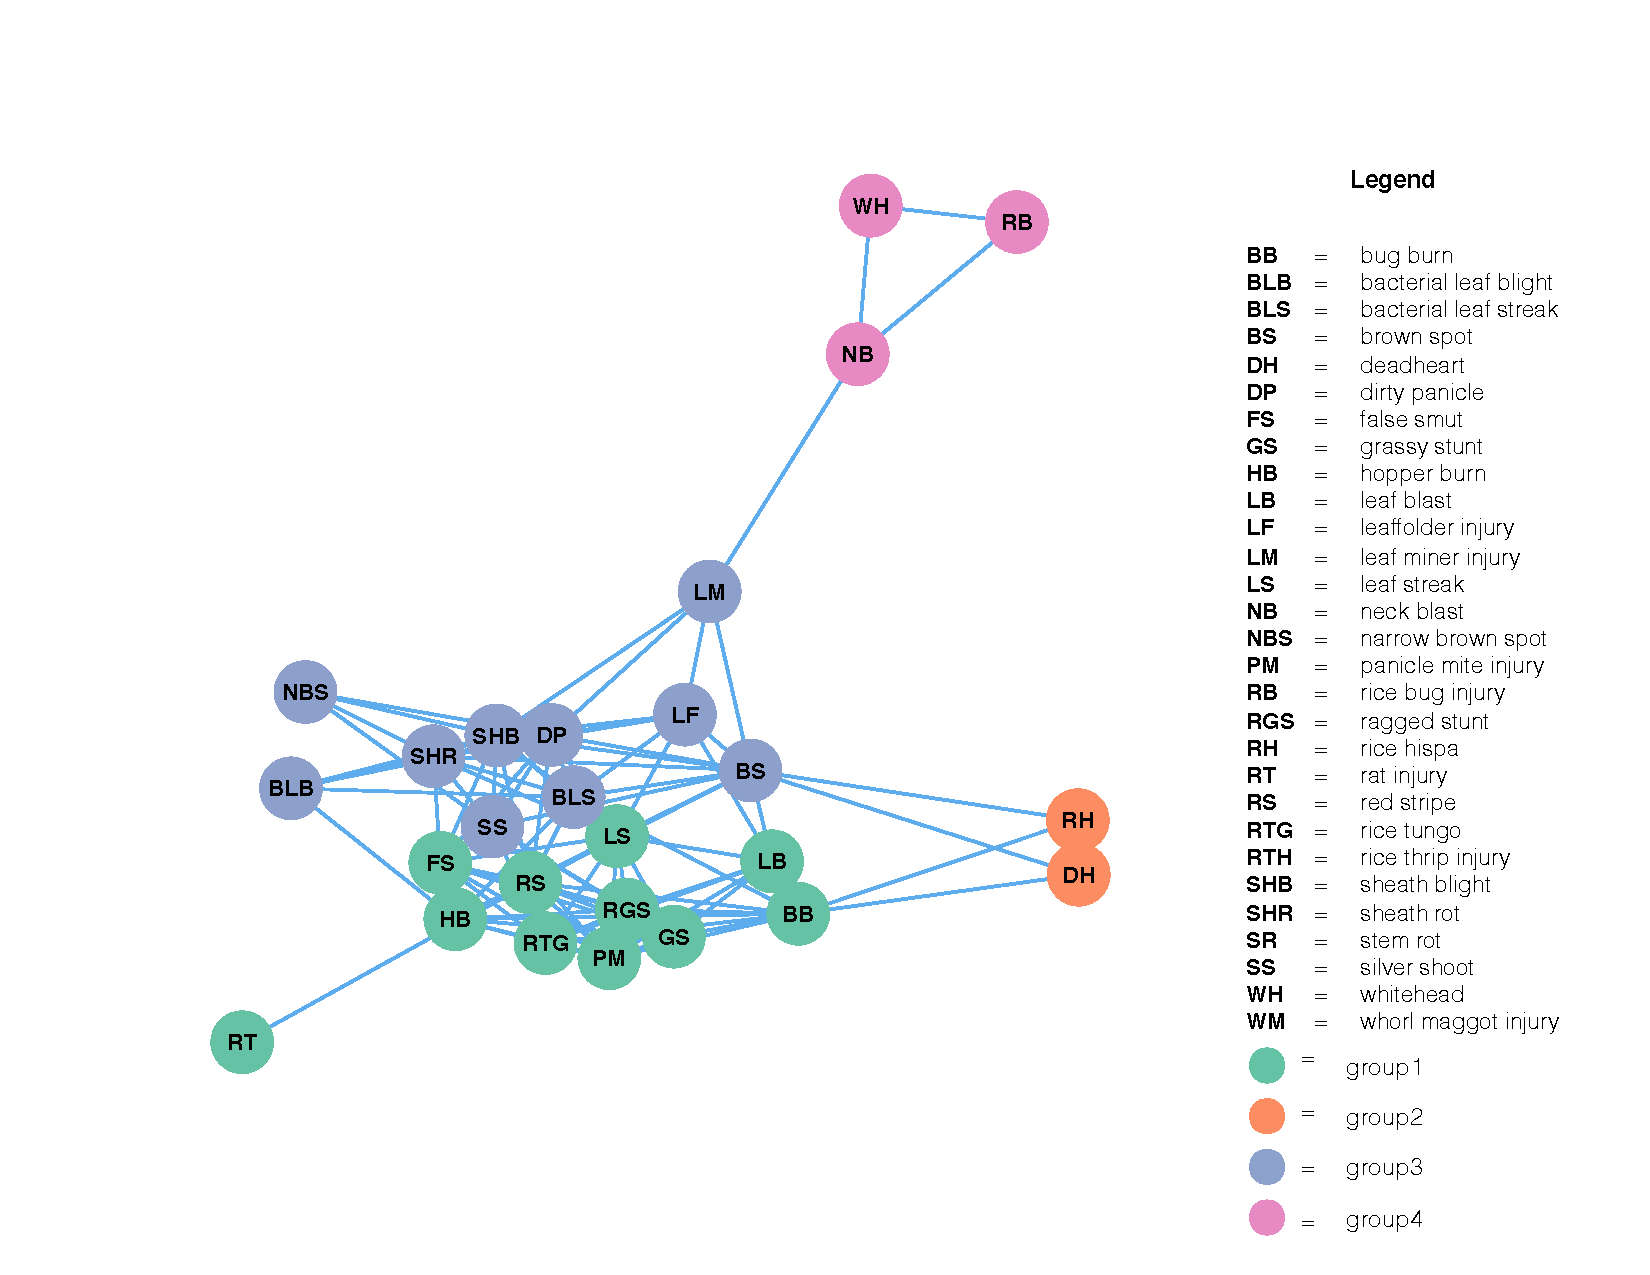
\includegraphics[width = 1\textwidth]{figures/networkWJ_ds/networkWJ_ds.pdf}
        \caption{Co-occurrence network of rice injuries in dry season at West Java, Indonesia. The layout of the network graph is based on the Fruchterman-Reingold algorithm, which places nodes with stronger or more connections closer to each other.}
        \label{fig:networkWJ_ds}
    \end{subfigure}
    \begin{subfigure}[b]{1\textwidth}
        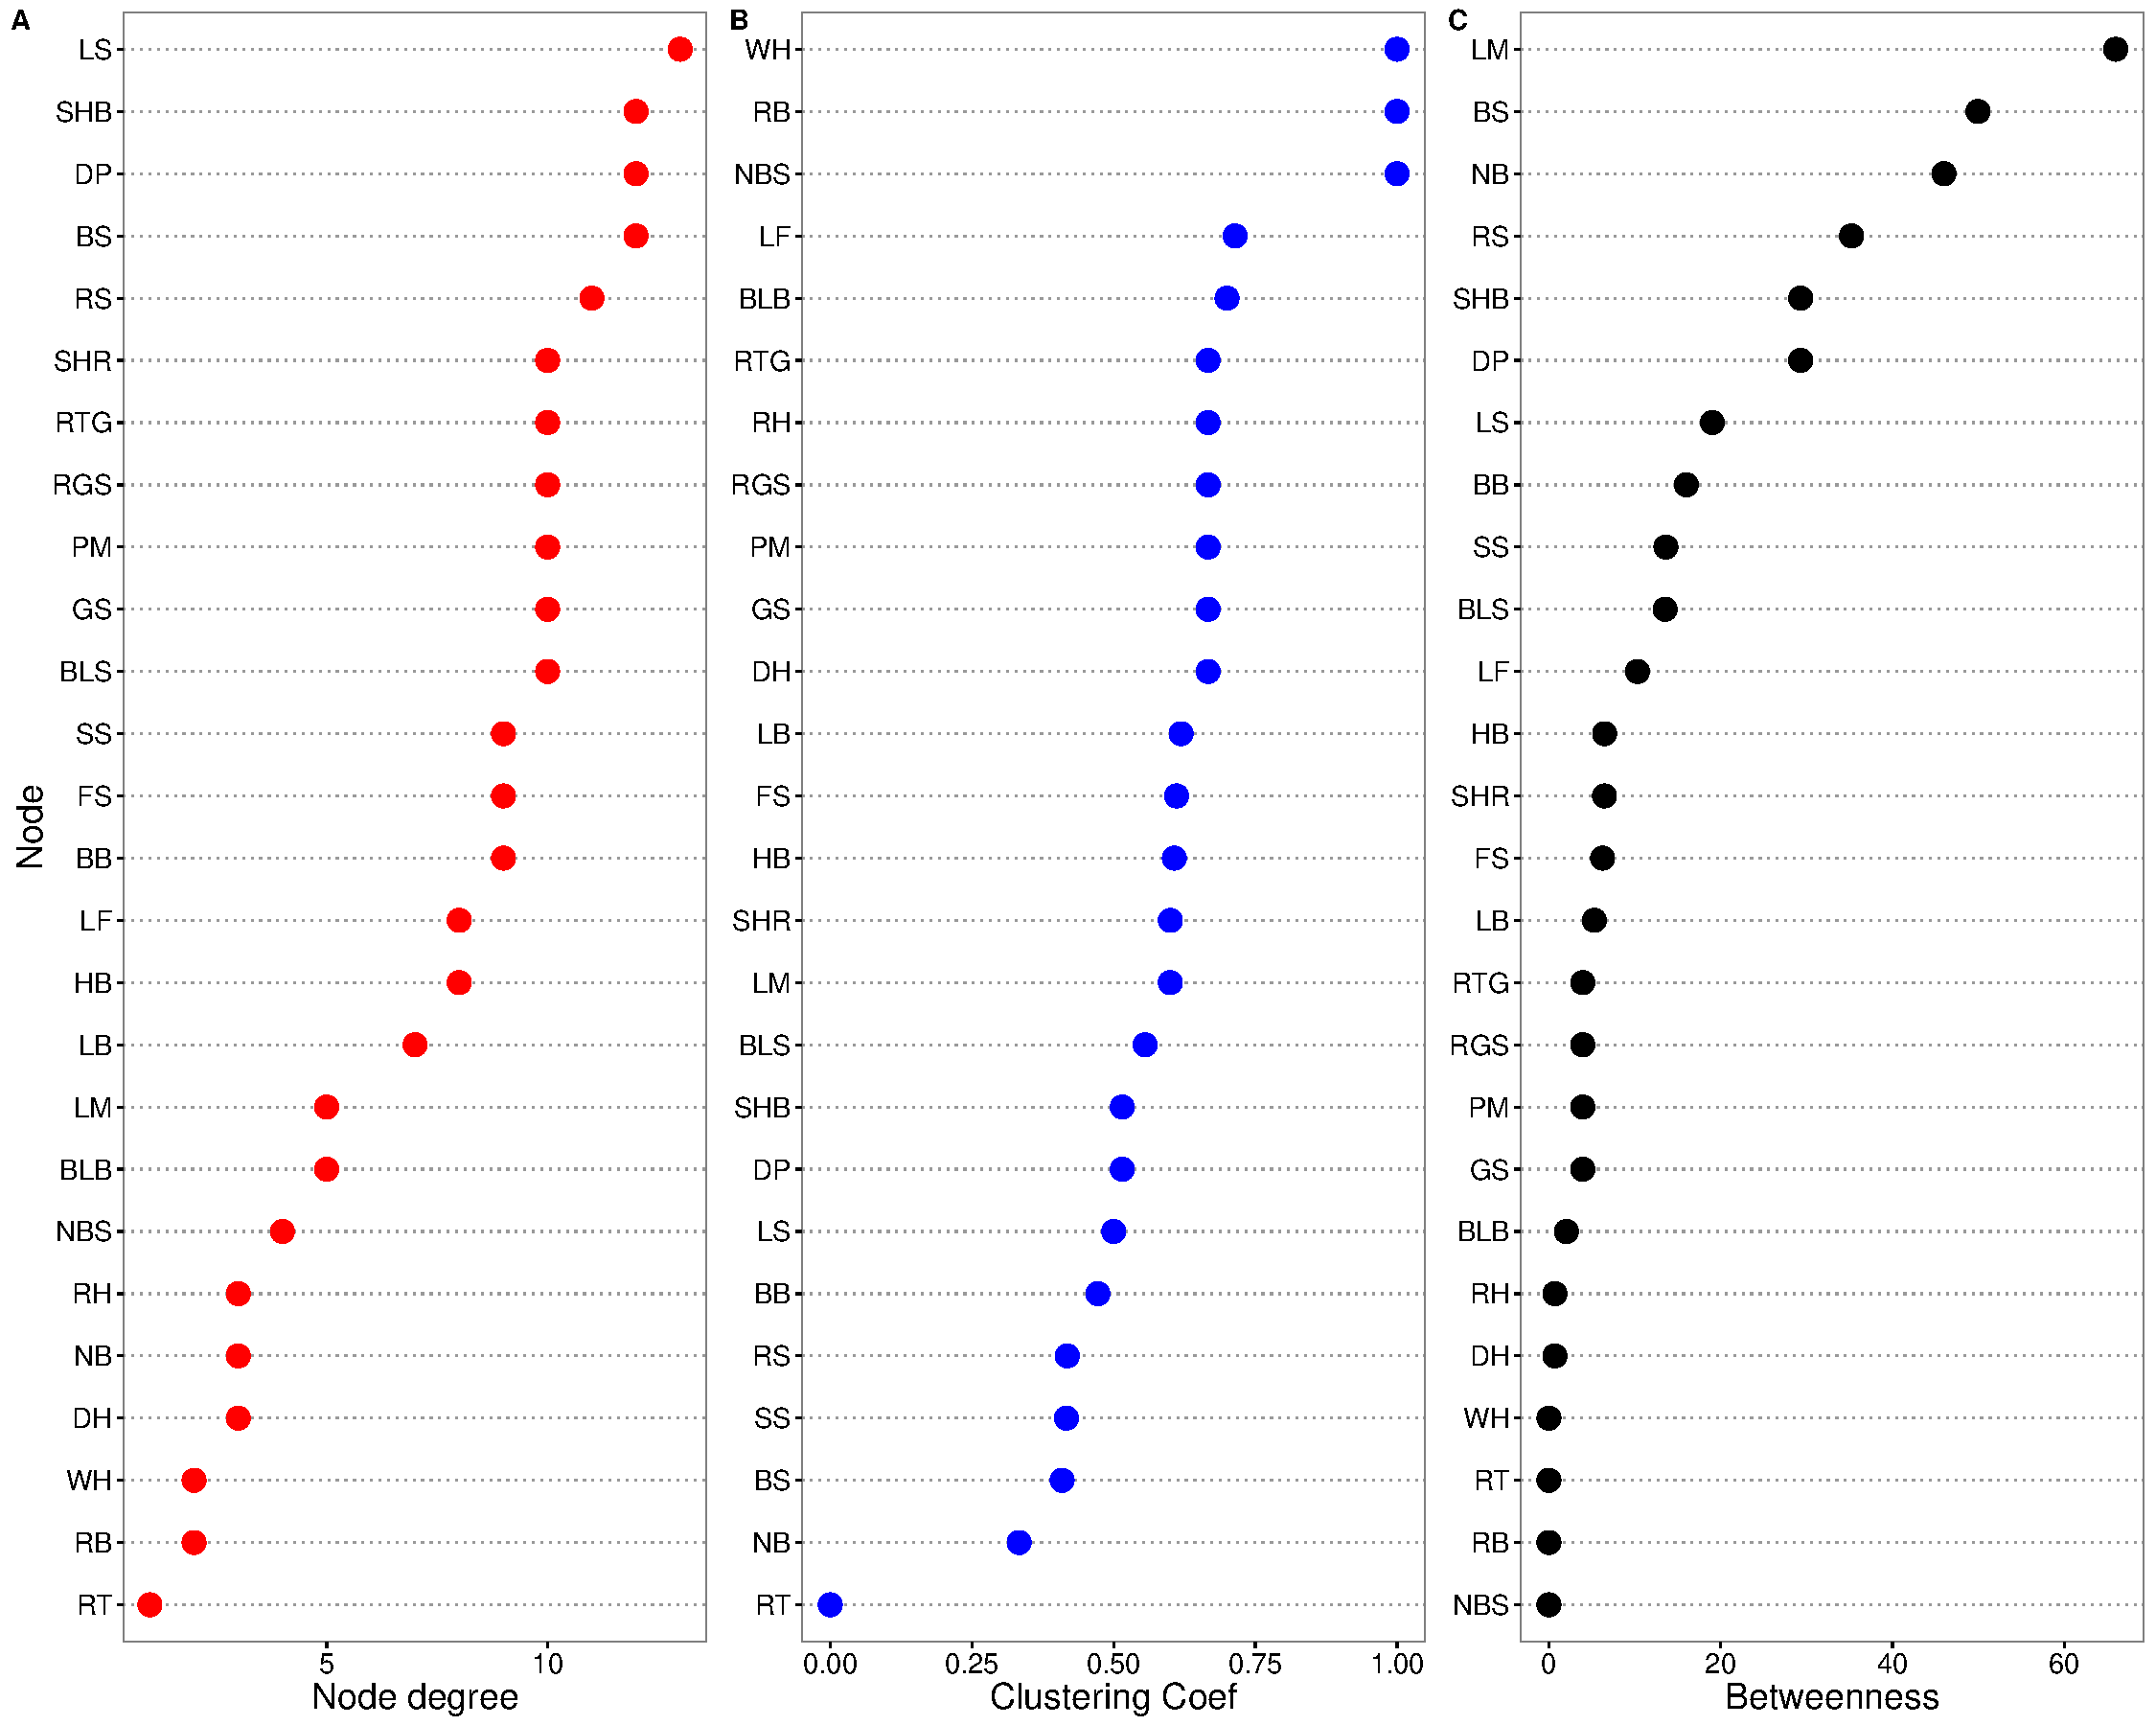
\includegraphics[width = 1\textwidth]{figures/nodepropWJ_ds/nodepropWJ_ds.pdf}
        \caption{Three centrality measures of the nodes in co-occurrence network of rice injuries in dry season at West Java, Indonesia. A: node degree, B:clustering coefficient, and C:Betweenness.}
        \label{fig:nodepropWJ_ds}
    \end{subfigure}
    \caption{Rice injuries in dry season in West Java, Indonesia}
    \label{fig:WJ_ds}
\end{figure}

\begin{figure}
    \centering
    \begin{subfigure}[b]{1\textwidth}
        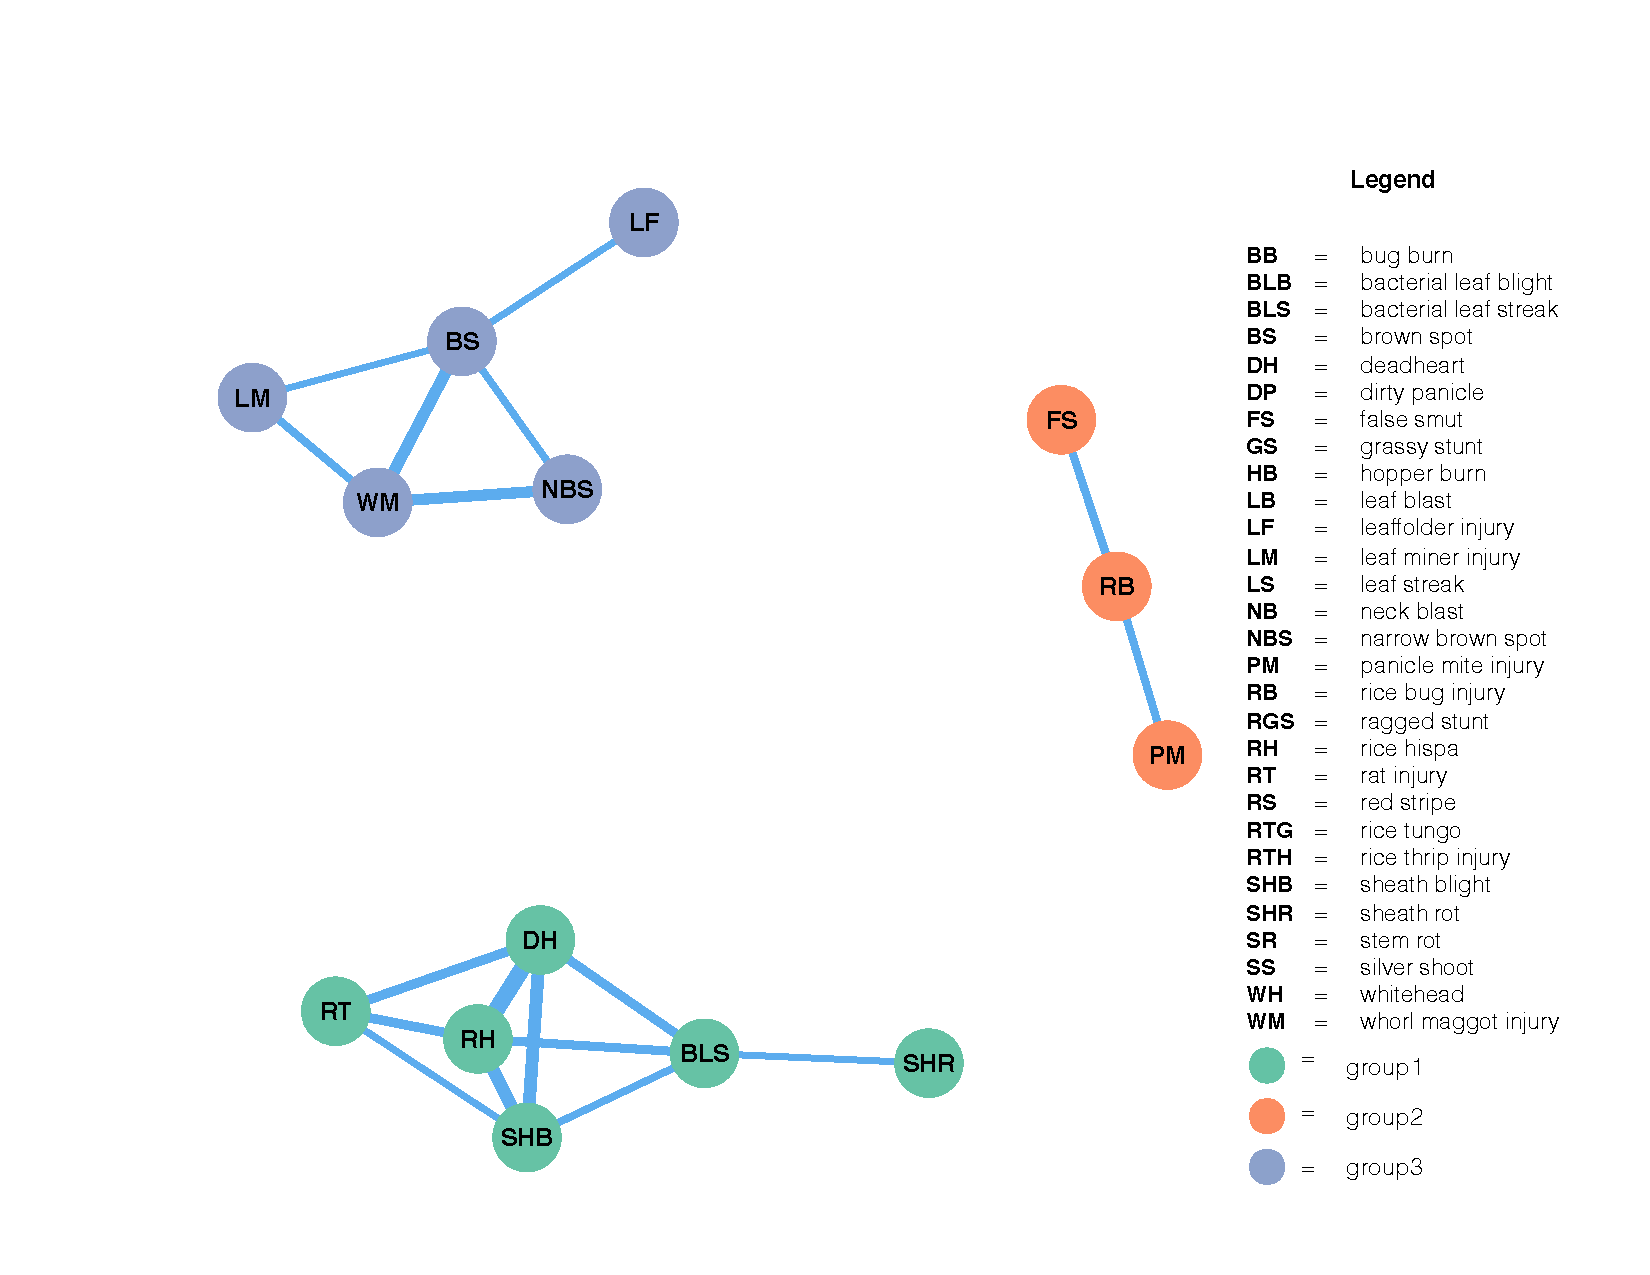
\includegraphics[width = 1\textwidth]{figures/networkWJ_ws/networkWJ_ws.pdf}
        \caption{Co-occurrence network of rice injuries in wet season at West Java, Indonesia. The layout of the network graph is based on the Fruchterman-Reingold algorithm, which places nodes with stronger or more connections closer to each other.}
        \label{fig:networkWJ_ws}
    \end{subfigure}
    \begin{subfigure}[b]{1\textwidth}
        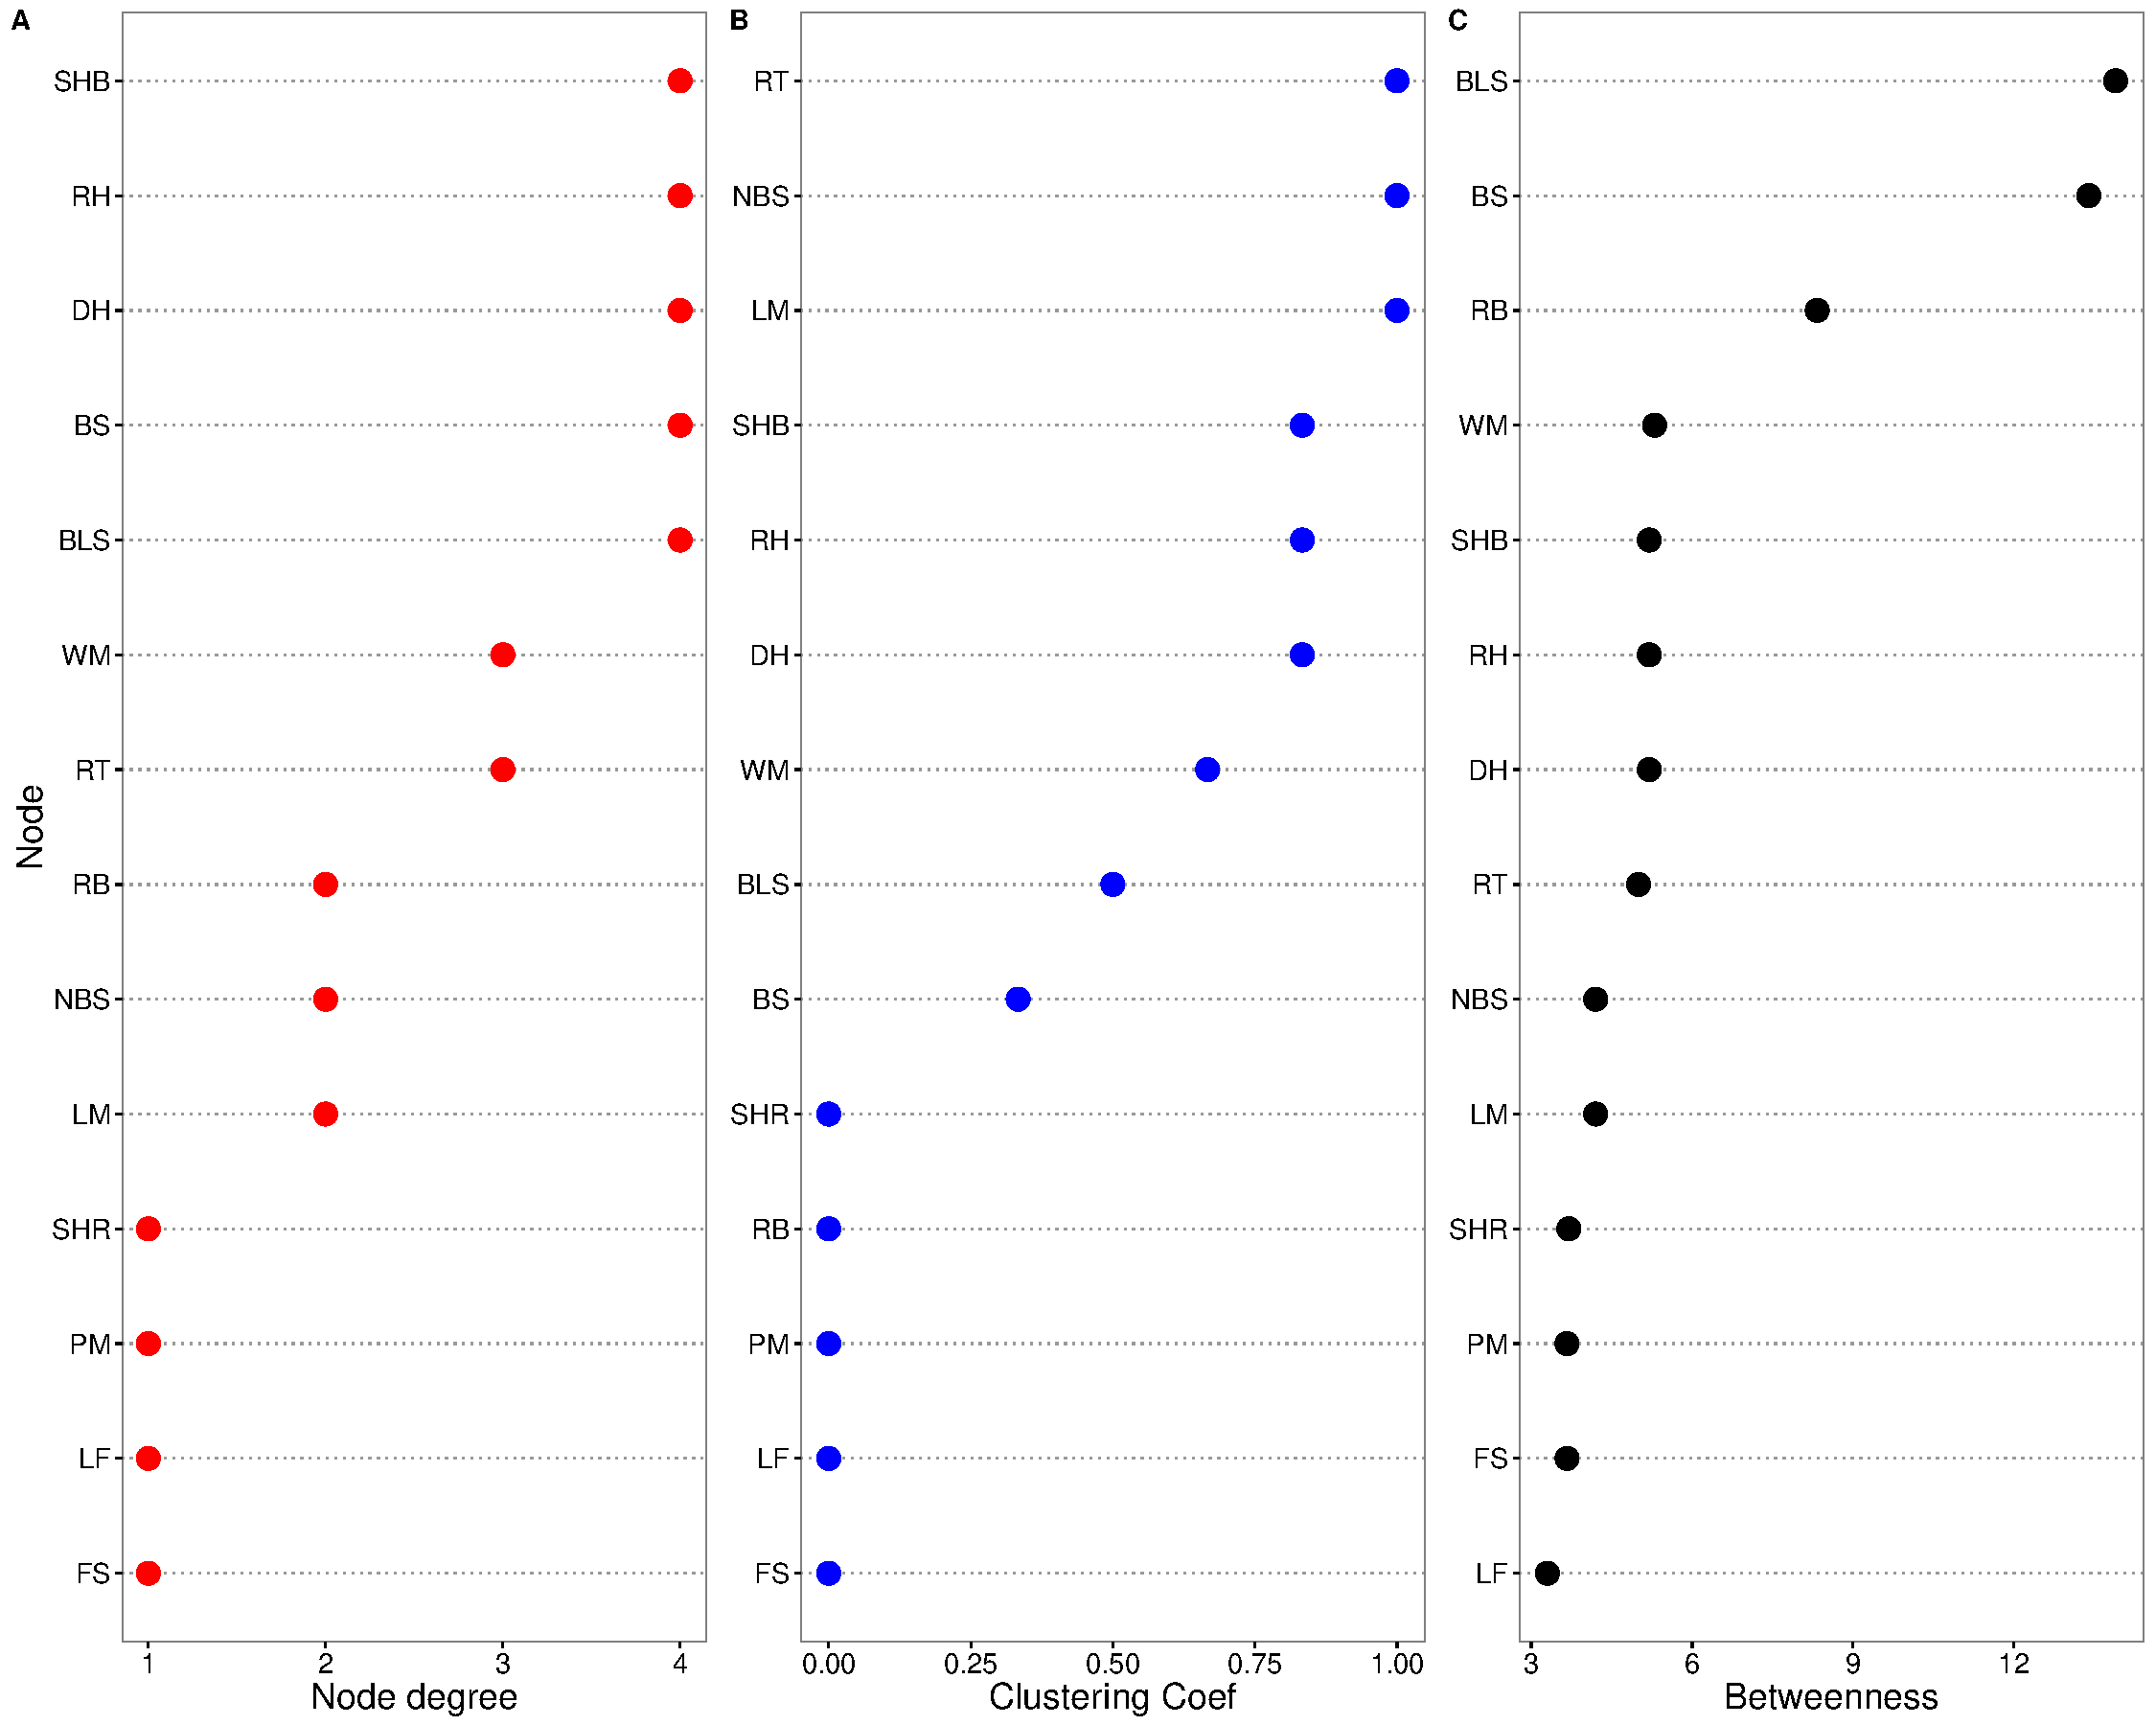
\includegraphics[width = 1\textwidth]{figures/nodepropWJ_ws/nodepropWJ_ws.pdf}
        \caption{Three centrality measures of the nodes in co-occurrence network of rice injuries in wet season at West Java, Indonesia. A: node degree, B:clustering coefficient, and C:Betweenness.}
        \label{fig:nodepropWJ_ds}    \end{subfigure}    \caption{Rice injuries in wet season in West Java, Indonesia}    \label{fig:WJ_ws}\end{figure}

\subsection{Discussion}
% Survey data
Rice injuries caused by animals, and pathogens were found commonly in South and South east Asia, but at different levels of incidence. Injuries indeed depended on locations or climate conditions favorable to develop \citep{Savary_2006_Quantification}. So they were not observed at all production environments or season during survey were conducting. For example, red stripe was often found in Central Plain, and West Java in dry season. 

%Using correlation
The co-occurrence correlations of rice injuries were explored using network inference based on strong and significant correlations through using non-parametric Spearman’s rank coefficient. Usually, correlations were assessed using Pearson correlation. However, the use of the Pearson correlation coefficient is problematic because it requires the variables are applied with similar measure, and the variable values are normally distributed. Additionally, Pearson correlation can only capture linear relationships. Due to the fact that the assumptions of Pearson correlation are not fit with the survey data. The alternative is provided by using Spearman’s rank correlation coefficient, which is also widely used in biological, and ecological studies
  

The exploration of co-occurrence networks is a useful method for determining interactions of co- occurring injuries. The centrality of nodes is considered further. The node centrality is the identification of which nodes are ``central’’ than others \citep{Barrat_2004_Architecture}. \citet{Newman_2003_Structure} mentioned three measures of node centrality: node degree, clustering coefficient, and betweenness. The node degree is measured by the number of connections a node has. In co-occurrence networks of rice injuries, node degree of each injury was counted from the number of the positive relationships of injuries have with other injuries. The clustering coefficient measure a density of local connectivity. Higher clustering coefficient of an element, the higher is the relationship among their neighbors. In the context of theses co-occurrence networks, nodes with high clustering coefficients were located closely. This indicated that they strongly occur together; one increasingly occurred, the related one also occurred jointly. In biological network, betweenness is used for measuring has been of how central a node is in a network, because a node with high betweenness essentially play an important role as a bridge between different parts of the network \citep{Proulx_2005_Network, Newman_2010_Networks}. In this study, nodes with high betweenness could be represented as indicators. Because theses nodes have many connections passed through, they are likely to be induced, and have higher chance to occur before other injuries associated.

Peripheral nodes or low-centrality nodes are also interesting. Ecological studies considered theses nodes as  specialists that have a few links and link specially to curtain nodes \citep{Lu_2013_Soil, Borthagaray_2014_Inferring}. In the context of co-occurrence networks of injuries, peripheral nodes have a few relationships within their groups in the network. They also slightly depend on other injuries. This may imply that these injuries are difficult to control because they may occurred occasionally such as rat injury (RT) in dry season at West Java, Indonesia, neck blast (NB) in wet season, in Tamil Nadu, bacterial leaf streak (BLS) in Red  River Delta, bacterial leaf blight (BLB), rat injury (RT) and sheath blight (SHB) in wet season at Odisha, India

%Dry vs Wet season
In the network of dry season in West Java, Indonesia, BLB and SR can be the targets to be monitored because they have high betweenness, which indicated that they are more likely to present then others injuries. Even though, the groups of injury profiles from this study are different from seasons and countries, but they are reasonable because some rice injuries present in some seasons (seasonal occurrence) such as gall midge injury \cite{Krishnaiah_2004_Rice}. The result also showed similar groups of injuries to the patterns of injuries profile from the study of \cite{Savary_2000_Characterization}. 

%SR is also best to be the target because it also associated with the RS, which has high clustering coefficients also because RS is potentially able to be co-found with many other injuries.  BLB also show the association with the injuries, which present high clustering coefficient. Both of BLB and SR are intermediate clustering coefficient., so they are formed concurrence between groups, but less potentially to present complex association. DH and WH are less associated with other injuries, so they are difficult to employ other injuries to. 

It is the good to monitored WM and RB and SHB also even the GLH has no betweenness, but it has high clustering coefficients, and connected with two high betweenness node. It would be also good target to monitored also because when it present, it also frequency appear together.
We explored the characteristics of rice injury profiles

With regard to pest management development, understanding that the relationships of rice injuries could simplify pest management decisions. As applied here, the node degree, clustering coefficients, and betweenness described the interaction of injuries in the networks. Therefore, they may be useful in finding a good indicator for monitoring pest in rice fields. High-betweenness node High- clustering coefficient node 

Community structures in networks can reveal hidden information that is maybe not easy to detect by simple observation. In social studies, community detection has been applied to search the groups of people who are interested in same topics.   In this study, I detected node community based on the optimization of the modularity of a sub-network, which is a popular approach \cite{Liu_2014_Detecting}. Communities are groups that are densely connected among their members, and sparsely connected with the rest of the network. Community structure can reveal abundant hidden information about complex networks that is not easy to detect by simple observation. Communities in a co-occurrence network of rice injuries might represent the rice injury co-occurrence association under related conditions. For example, the network of dry season in Central Plain revealed that group2 (LB, WM, LF and BLB).  According to \citet{Savary_2000_Characterization}, these injuries were in injuries profile group2 (IN2). \citet{Savary_2000_Characterization} also mentioned that IN2 was related to production situation group2 (PR2), this type was also dominantly found in direct seeded rice fields. So injuries in group2 of the network in dry season in CP could co-occur favorably in rice fields where applied direct seedling method, which is the most common practices in Thailand \citep{IRRI_2013_Rice}. 
\subsection{Conclusion}


Important challenges, however; remain in order to further rice injury characterization:
1
2
3
The study, illustrated that network methods offers a new set of exciting tools to classify, delimit and better understand the injury syndrome or injury profiles.

